\documentclass[11pt, oneside]{book}
\usepackage[paperwidth=17cm, paperheight=22.5cm, bottom=2.5cm, right=2.5cm]{geometry}

% El borde inferior puede parecerles muy amplio a la vista. Les recomiendo hacer una prueba de impresión antes para ajustarlo

\usepackage{amssymb,amsmath,amsthm} % Símbolos matemáticos
\usepackage[spanish]{babel}
\usepackage[utf8]{inputenc} % Acentos y otros símbolos 
\usepackage{enumerate}
\usepackage[hidelinks]{hyperref} % Hipervínculos en el índice
\usepackage{graphicx}
%\usepackage{subfig} % Subfiguras
\graphicspath{{Imagenes/}} % En qué carpeta están las imágenes

% Para eliminar guiones y justificar texto
\tolerance=1
\emergencystretch=\maxdimen
\hyphenpenalty=10000
\hbadness=10000

\linespread{1.25} % Asemeja el interlineado 1.5 de Word

\let\oldfootnote\footnote % Deja espacio entre el número del pie de página y el inicio del texto
\renewcommand\footnote[1]{%
\oldfootnote{\hspace{0.05mm}#1}}

\renewcommand{\thefootnote} {\textcolor{Black}{\arabic{footnote}}} % Súperindice a color negro

\setlength{\footnotesep}{0.75\baselineskip} % Espaciado entre notas al pie

\usepackage{fnpos} % Footnotes al final de pág.

\usepackage[justification=centering, font=bf, labelsep=period, skip=5pt]{caption} % Centrar captions de tablas y ponerlas en negritas

\newcommand{\imagesource}[1]{{\footnotesize Fuente: #1}}

\usepackage{tabularx} % Big tables
\usepackage{graphicx}
\usepackage{adjustbox}
\usepackage{longtable}

\usepackage{float} % Float tables

\usepackage[dvipsnames]{xcolor} % Color

\usepackage{pgfplots} % Gráficas
\pgfplotsset{compat=newest}
\pgfplotsset{width=7.5cm}
\pgfkeys{/pgf/number format/1000 sep={}}

\begin{document}

%----------------------------------------------------------------------------------------
%	PORTADA
%----------------------------------------------------------------------------------------

\title{El efecto causal de las cámaras de velocidad en el número de incidentes viales en la Ciudad de México} % Con este nombre se guardará el proyecto en writeLaTex

\begin{titlepage}
\begin{center}

\textsc{\Large Instituto Tecnológico Autónomo de México}\\[2em]

%Figura
\begin{figure}[h]
\begin{center}

\includegraphics[scale=0.50]{itam_logo.png}
\end{center}
\end{figure}

% Pueden modificar el tamaño del logo cambiando la escala

\textbf{\LARGE El efecto causal de las cámaras de velocidad en el número de incidentes viales en la Ciudad de México}\\[2em]

\textsc{\large Tesis}\\[1em]

\textsc{\large que para obtener el título de}\\[1em]

\textsc{\LARGE Licenciado en Ciencia de Datos}\\[1em]

\textsc{\large Presenta}\\[1em]

\textsc{\LARGE Mariano Alcaraz Aguilar}\\[4em]

\textsc{\large ASESOR: DR. ALBERTO SIMPSER MONDLAK}\\[.8em]


% Asegúrense de escribir el nombre completo de su asesor

\end{center}

\vspace*{\fill}
\textsc{Ciudad de México \hspace*{\fill} 2025}

\end{titlepage}

%----------------------------------------------------------------------------------------
%	DECLARACIÓN
%----------------------------------------------------------------------------------------

\thispagestyle{empty}

\vspace*{\fill}
\begingroup

\noindent
«Con fundamento en los artículos 21 y 27 de la Ley Federal del Derecho de Autor y como titular de los derechos moral y patrimonial de la obra titulada ``\textbf{El efecto causal de las cámaras de velocidad en el número de incidentes viales de la Ciudad de México}'', otorgo de manera gratuita y permanente al Instituto Tecnológico Autónomo de México y a la Biblioteca Raúl Bailléres Jr., la autorización para que fijen la obra en cualquier medio, incluido el electrónico, y la divulguen entre sus usuarios, profesores, estudiantes o terceras personas, sin que pueda percibir por tal divulgación una contraprestación.»

% Asegúrense de cambiar el título de su tesis en el párrafo anterior

\centering 

\vspace{5em}

\rule[1em]{20em}{0.5pt} % Línea para la fecha

\textsc{Fecha}
 
\vspace{8em}

\rule[1em]{20em}{0.5pt} % Línea para la firma

\textsc{Mariano Alcaraz Aguilar}

\endgroup
\vspace*{\fill}

%----------------------------------------------------------------------------------------
%	DEDICATORIA
%----------------------------------------------------------------------------------------

\pagestyle{plain}
\frontmatter

\chapter*{}
\begin{flushright}
\textit{A mis padres,\\ por su incansable esfuerzo.}
\end{flushright}

%----------------------------------------------------------------------------------------
%	AGRADECIMIENTOS
%----------------------------------------------------------------------------------------

\chapter*{Agradecimientos}

\noindent Lorem ipsum dolor sit amet, consectetur adipiscing elit.

% Esta sección es lo único que la gente lee. True story :)

%----------------------------------------------------------------------------------------
%	RESUMEN
%----------------------------------------------------------------------------------------

\chapter*{Resumen}

\noindent Abstract goes here en español

\pagestyle{plain}

\noindent 

%----------------------------------------------------------------------------------------
%	Summary
%----------------------------------------------------------------------------------------

\chapter*{Summary}

\noindent Abstract goes here in English

\pagestyle{plain}

\noindent 

%----------------------------------------------------------------------------------------
%	TABLA DE CONTENIDOS
%---------------------------------------------------------------------------------------

\tableofcontents

%----------------------------------------------------------------------------------------
%	ÍNDICE DE CUADROS Y FIGURAS
%---------------------------------------------------------------------------------------

\listoftables

\listoffigures

%----------------------------------------------------------------------------------------
%	TESIS
%----------------------------------------------------------------------------------------

\mainmatter % Empieza la numeración de las páginas

\pagestyle{plain}

% Incluye los capítulos en el fólder de capítulos

\chapter*{Introducción}
\addcontentsline{toc}{chapter}{Introducción}

% La introducción no cuenta como primer capítulo
\section{Motivación y contexto}
\noindent La siniestralidad vial en la Ciudad de México constituye un problema de salud pública de primer orden. Entre 2014 y 2023 la ciudad registró, en promedio, 85,150 accidentes viales anuales, con un saldo de 37,638 personas lesionadas y 383 defunciones al año, es decir, más de una muerte diaria solo en el lugar del incidente. Estas cifras, provenientes de los registros del Centro de Comando, Control, Cómputo, Comunicaciones y Contacto Ciudadano (C5), ilustran la magnitud del problema y sus implicaciones tanto para la seguridad vial como para el sistema de salud.\\
% aquí debe ir la sección que explica que el gobierno se ha dado cuenta del problema

% una vez que ya explicamos que el gobierno está conciente de que hay accidentes y que la velocidad es un problema entra la parte de las fotocívicas y de las fotomultas.
\indent Más allá del nivel absoluto de incidentes, la evolución reciente de estos eventos sugiere que la situación se ha vuelto especialmente preocupante en los últimos años. La Figura 1 muestra la trayectoria del número total de accidentes viales entre 2014 y 2023, desagregados en accidentes menores, con lesionados y fatales. El sistema de fotocívicas entró en vigor el 22 de abril de 2019. Hasta ese momento se observaba una tendencia a la baja tanto en el número total de incidentes como en los accidentes fatales anuales. Sin embargo, tras una caída pronunciada en 2020 ---muy probablemente asociada a la reducción de la movilidad durante la pandemia de COVID‑19--- se registra un repunte en el número de incidentes viales, especialmente en los de mayor severidad.

\begin{figure}
    \centering
    \caption{Número anual de incidentes viales en la CDMX}
    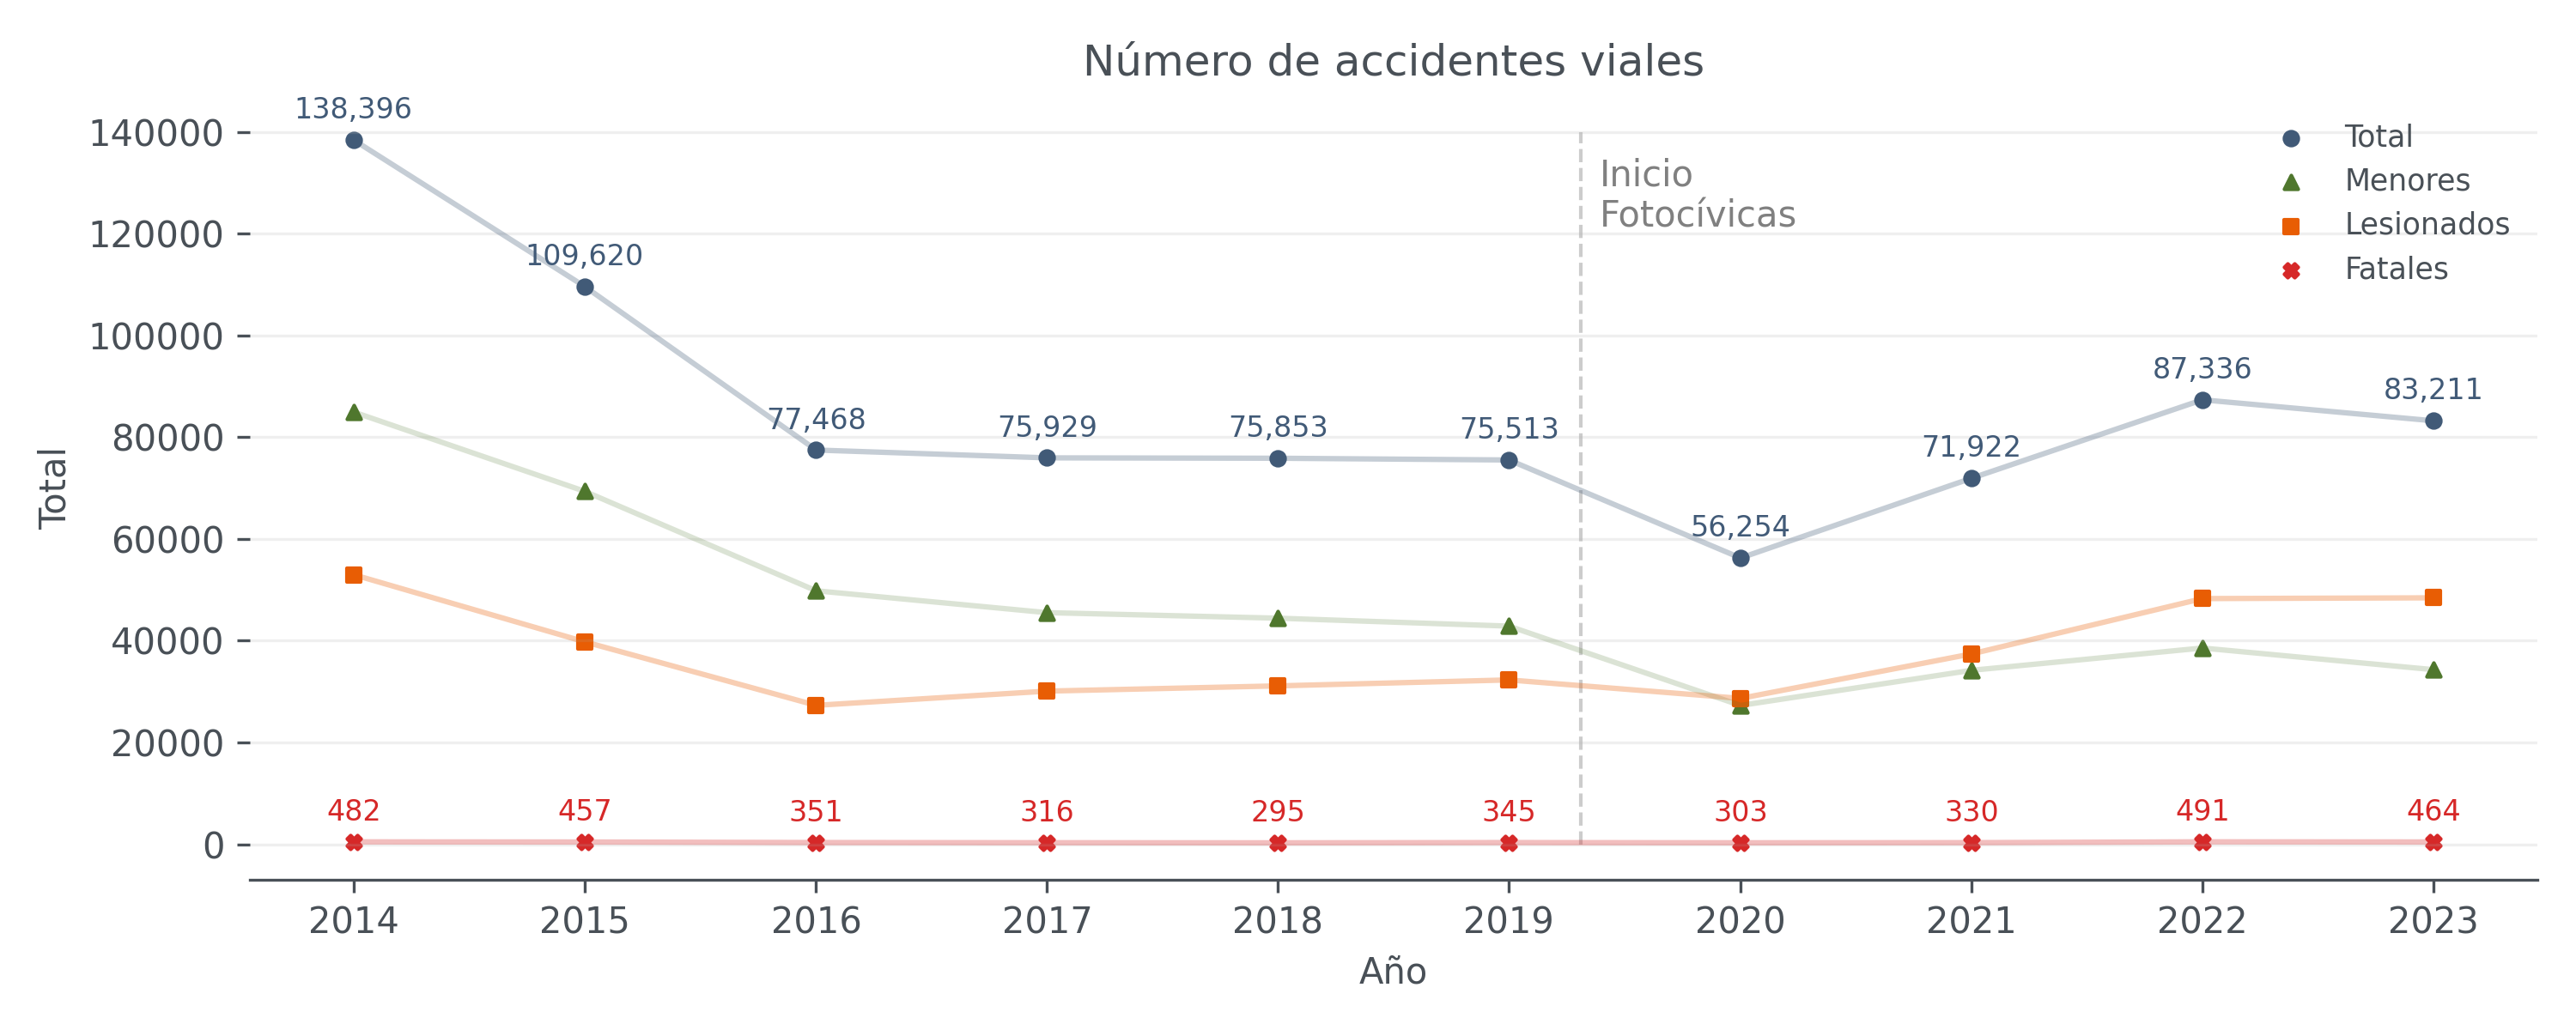
\includegraphics[width=1\linewidth]{Imagenes/yearly-number-of-incidents.png}
    \label{fig:placeholder}
\end{figure}

Este cambio de tendencia se aprecia con claridad al comparar 2018, último año completo previo a la implementación de las fotocívicas, con 2023. En ese periodo, los incidentes totales pasaron de 75,853 a 83,211, lo que implica un aumento de 9.7\%. Más grave aún, los accidentes con al menos una persona fallecida se incrementaron de 295 a 464, es decir, un aumento del 57\%. La Figura 2, que presenta únicamente el número de accidentes fatales por año, muestra un mínimo en 2018 seguido de un crecimiento sostenido. Aunque con esta evidencia descriptiva no es posible atribuir causalmente estos cambios a un solo factor, sí resulta claro que la introducción del programa de fotocívicas no evitó el repunte observado en los accidentes más graves en el total agregado de la ciudad.

\begin{figure}
    \centering
    \caption{Número anual de accidentes fatales}
    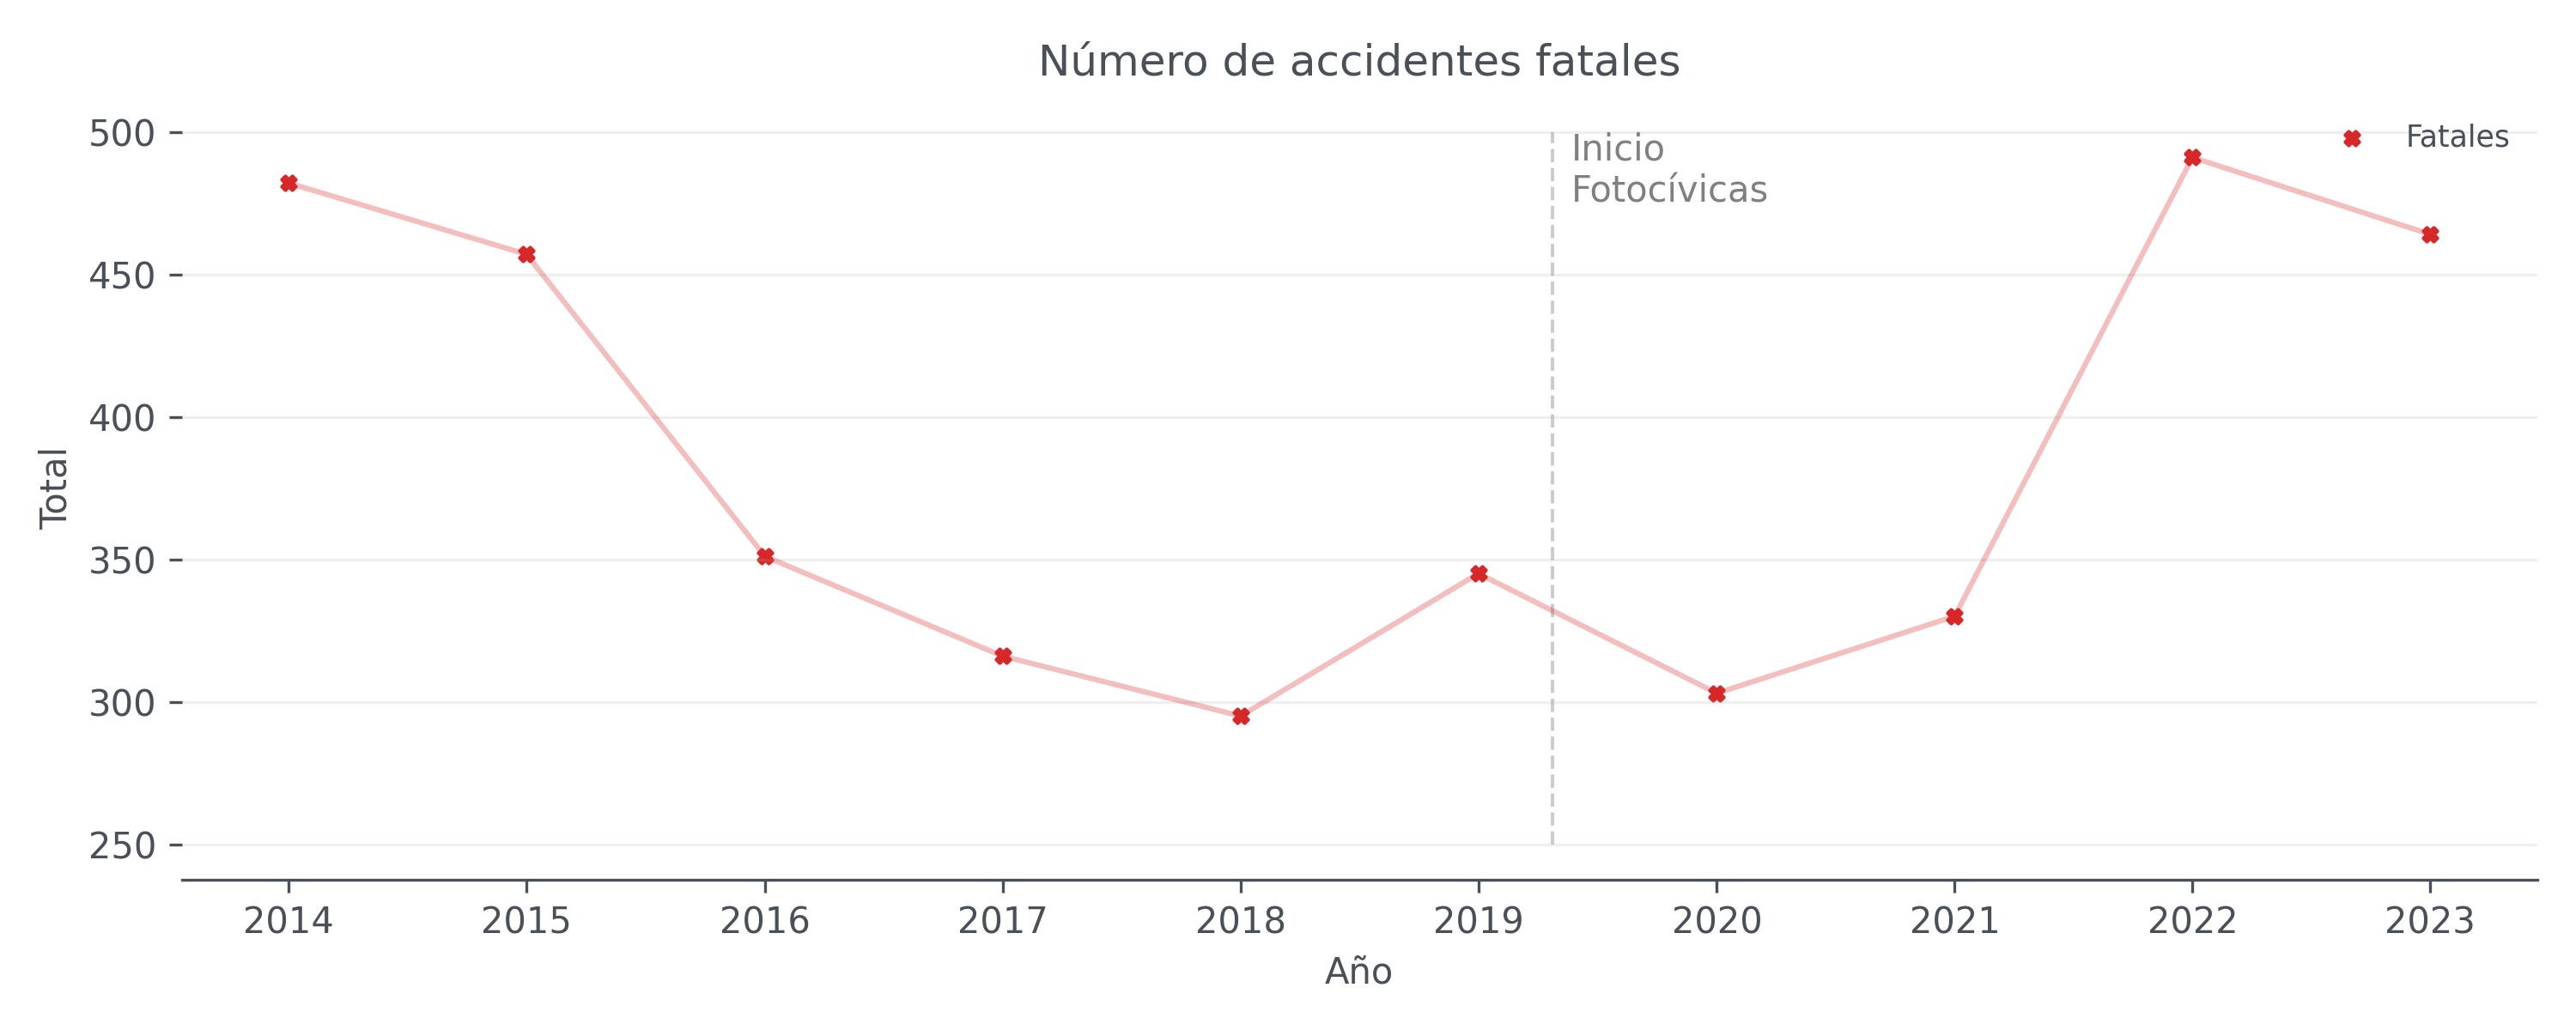
\includegraphics[width=1\linewidth]{Imagenes/yearly-fatal-number-of-incidents}
    \label{fig:figure-here}
\end{figure}

La composición de los siniestros también se ha modificado. Como se observa en la Figura 1, la disminución de 2020 en el número total de incidentes se explica principalmente por la reducción de los accidentes menores, mientras que los accidentes con lesionados o fallecidos no se reducen en la misma proporción. A partir de 2020, los incidentes con personas lesionadas superan a los accidentes considerados menores y se mantienen por encima hasta 2023, ampliando cada año la brecha entre ambos tipos de eventos. Es decir, no solo sigue habiendo muchos accidentes, sino que una fracción creciente de ellos tiene consecuencias más severas.\\

Este diagnóstico coincide con lo reportado por la Secretaría de Movilidad (SEMOVI) en el Programa Integral de Seguridad Vial de la Ciudad de México 2021–2024, donde se documenta que la reducción en la afluencia vehicular durante la pandemia ---aproximadamente del 45\%--- permitió mayores velocidades de circulación y que el aumento relativo de incidentes con lesionados y fallecidos se concentró en vías primarias y de acceso controlado. En otras palabras, el propio gobierno local reconoce que la velocidad y las características de la infraestructura vial juegan un papel central en la siniestralidad reciente.\\ 

Para analizar este fenómeno y evaluar la efectividad de las intervenciones de control de velocidad es necesario contar con información adecuada sobre los incidentes viales. Existen diversas fuentes de datos que ofrecen perspectivas complementarias. Por un lado, la Secretaría de Seguridad Ciudadana (SSC) publica registros georreferenciados de hechos de tránsito a partir de junio de 2018, pero estos datos solo incluyen incidentes con personas lesionadas y cubren un periodo relativamente corto en relación con la entrada en vigor del sistema de fotocívicas, lo que dificulta construir una ventana simétrica de al menos tres años antes y después de la política.\\

Por otro lado, los datos del C5 ofrecen una cobertura temporal más amplia y un panorama más completo de la siniestralidad. Esta base integra reportes de llamadas al 911, incidentes detectados por las cámaras de videovigilancia y registros levantados por las autoridades en el lugar de los hechos. Además, incluye tanto accidentes con lesionados y fallecidos como incidentes menores, que de otra forma quedarían subrepresentados. Por estas razones, en esta tesis empleo los registros del C5 como fuente principal para el análisis.\\ 

\section{Programas de control de velocidad en la Ciudad de México}
\noindent El control de la velocidad ha adquirido relevancia mundial como estrategia central para mejorar la seguridad vial. La Guía para el Control de la Velocidad (Secretaría de Salud, 2018) identifica la velocidad como el principal factor de riesgo en la ocurrencia y severidad de los siniestros viales y destaca que “el 90\% de los automovilistas se considera un conductor por encima del promedio y de bajo riesgo”. Esta sobreconfianza convive con una infraestructura pensada para favorecer traslados rápidos y con una cultura que valora la velocidad por encima de la seguridad. La misma guía documenta que la probabilidad de sobrevivir a un atropellamiento se reduce de 90\% a 30 km/h a solo 17\% a 50 km/h, lo que refuerza la necesidad de limitar las velocidades efectivas en la red vial.\\

\indent En la Ciudad de México, la principal herramienta de control automatizado de la velocidad han sido los programas de fotomultas y, posteriormente, de fotocívicas. El Programa Fotomultas comenzó a operar en diciembre de 2015 con un diseño claramente recaudatorio: el exceso de velocidad detectado por los radares se traducía en sanciones económicas aplicadas al propietario del vehículo. Este esquema fue objeto de críticas por su orientación a la recaudación y por la falta de transparencia en la operación.\\

En abril de 2019 el gobierno de la ciudad sustituyó el esquema de fotomultas por el sistema de fotocívicas, con el argumento de transitar de una política centrada en la recaudación hacia una enfocada en el cambio de conducta. El nuevo modelo se basa en un sistema de puntos asociado a las placas de los vehículos registrados en la ciudad: cada placa inicia con diez puntos y, por cada infracción detectada, se pierde un punto (cinco puntos si el límite de velocidad se excede en más de 40\%). La forma de resarcir estas infracciones ya no es el pago de una multa, sino la realización de cursos educativos y trabajo comunitario. Cuando una placa pierde más de dos puntos, su propietario no puede verificar el vehículo hasta cumplir con las sanciones correspondientes (no es posible circular si el vehículo no está verificado). Para los vehículos con placas foráneas, en cambio, el esquema mantiene las sanciones económicas.\\

La implementación de fotocívicas vino acompañada de una reubicación de los radares. De acuerdo con la SEMOVI, las cámaras se reubicaron hacia tramos con mayor incidencia de hechos de tránsito, en particular aquellos con más muertos y lesionados, así como en puntos con elevados volúmenes de tránsito y donde el límite de velocidad tendía a no respetarse. En total se instalaron 138 dispositivos, de los cuales 58 provenían del sistema anterior y 80 fueron nuevos. Aunque la lógica oficial no menciona explícitamente indicadores como el exceso medio de velocidad, sí enfatiza la concentración de incidentes y la importancia de las vías primarias y de acceso controlado como criterio de ubicación.\\

En la práctica, sin embargo, el nuevo sistema ha seguido funcionando en gran medida como un esquema de sanciones económicas. Los registros de la propia autoridad, como lo podemos observar en la Figura 3, muestran que la proporción de sanciones cívicas ha oscilado entre 14\% y 24\% del total, lo que implica que la mayoría de las infracciones se ha traducido en multas monetarias. Esto puede deberse, entre otras razones, al elevado número de vehículos con placas foráneas que circulan por la ciudad o a que los propietarios con placas locales internalizan mejor el riesgo de sanción y ajustan su comportamiento. Aunque el análisis detallado de estas causas excede el alcance de esta tesis, el dato es relevante porque sugiere que la experiencia de los conductores con el sistema se asemeja más a un esquema de multas que al modelo cívico originalmente planteado.\\

\begin{figure}
    \centering
    \caption{Total de infracciones por tipo de sanción}
    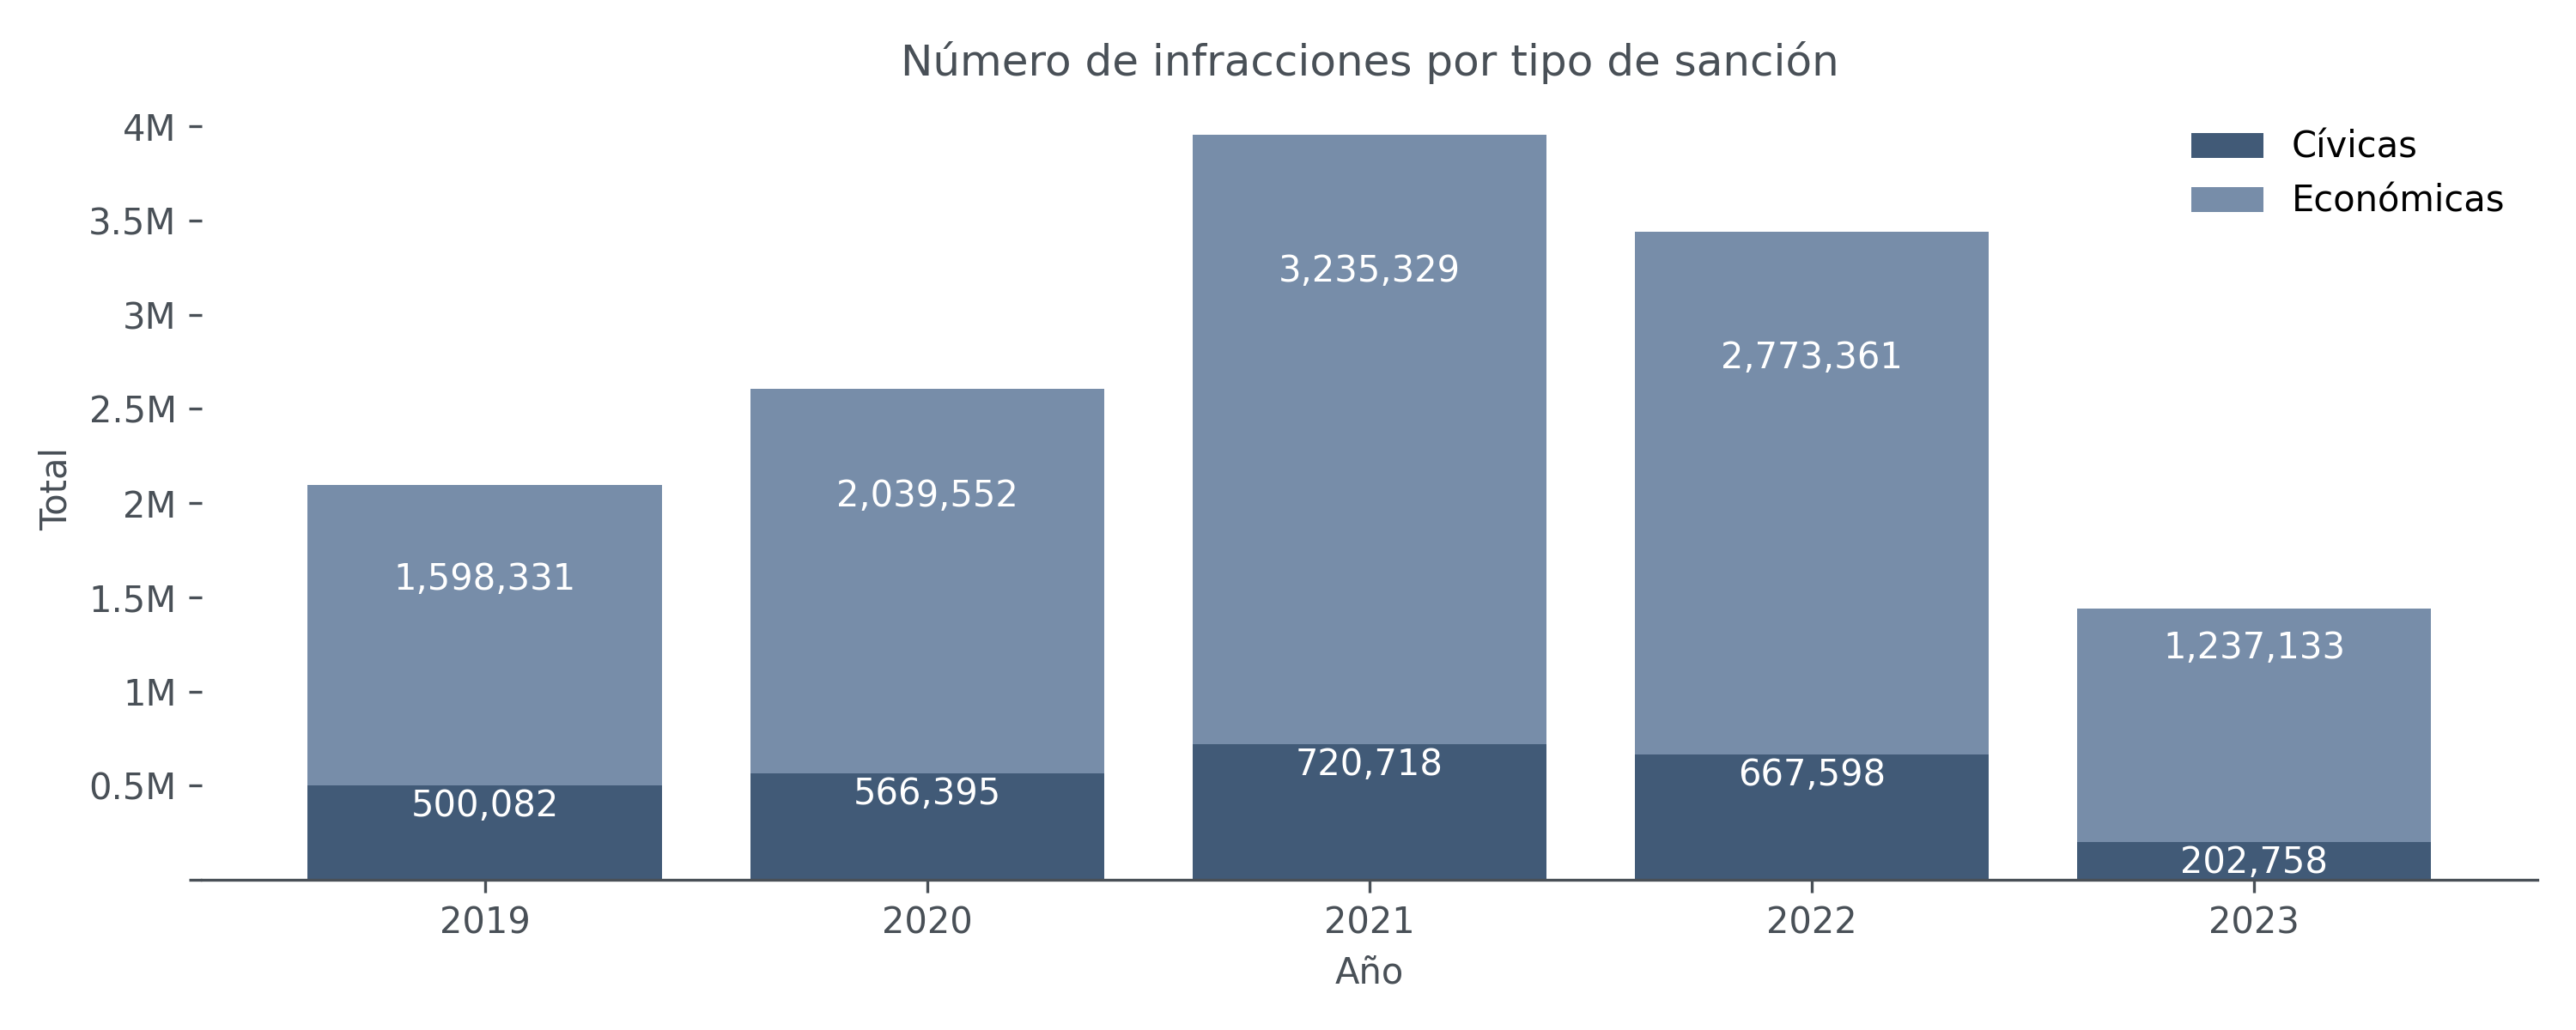
\includegraphics[width=1\linewidth]{Imagenes/yearly-number-of-sanctions.png}
\end{figure}

\section{Pregunta de investigación e hipótesis}
\noindent En este contexto, es natural preguntarse si las cámaras de velocidad realmente han tenido el efecto que prometían sobre la seguridad vial de la ciudad. A primera vista, podría pensarse que, al menos en los puntos donde se instalaron, deberían observarse menos incidentes, en particular menos hechos con personas lesionadas o fallecidas. Sin embargo, las tendencias mostradas en las figuras anteriores, así como el repunte reciente de los accidentes fatales, hacen que esta intuición deje de ser tan obvia. La pregunta que guía esta tesis es precisamente esa: \textbf{¿qué tanto han cambiado los incidentes viales en torno a las cámaras de velocidad desde la implementación del sistema de fotocívicas?}\\

En esta tesis parto de la hipótesis de que las cámaras de velocidad del sistema de fotocívicas reducen el número de incidentes viales en su entorno, con un efecto relativamente mayor en los siniestros más graves (con lesionados y, sobre todo, con fallecidos), en magnitudes similares a las reportadas en la literatura internacional (del orden de 10–20\%). Para poner a prueba esta hipótesis utilizo los registros del C5 y construyo unidades de análisis espaciales. Primero ensayo un enfoque basado en una malla de cuadrículas sobre toda la ciudad, pero encuentro que los resultados son muy sensibles a cambios mínimos en el diseño del grid, lo que revela problemas de robustez y me lleva a descartar este esquema.\\

A partir de ello adopto un segundo método, inspirado en trabajos como Li et al. (2020), que define áreas circulares alrededor de cada cámara. Construyo para cada una un grupo de control mediante Propensity Score Matching, usando como covariables la siniestralidad previa, características de la infraestructura vial y proxies de movilidad basados en afluencia al metro y radares de conteo de tránsito vehicular. Para estimar los efectos utilizo un método de Diferencia en Diferencias, evaluando la interacción del tiempo con el tratamiento en mis unidades tratadas contra las de control.\\

En términos generales, los resultados muestran que no existe evidencia estadística suficiente para afirmar que las cámaras generaron una reducción localizada de la siniestralidad en su entorno inmediato. Al mismo tiempo, sí se observa una caída agregada de los incidentes en áreas tratadas y de control después de la implementación del programa, lo que sugiere que la evidencia previa para la ciudad puede estar captando cambios sistémicos más que efectos causales estrictamente locales alrededor de los radares.

\section{Contribuciones a la literatura}
\noindent Solo es posible entender la justificación de esta tesis bajo el contexto de la literatura existente en la Ciudad de México, pues no es el primer estudio que analiza el efecto de las cámaras de velocidad en la siniestralidad vial. Bajo este supuesto, es más fácil ver cómo encaja precisamente ahí donde hay oportunidades de traer lo que la literatura internacional ha encontrado al contexto de la Ciudad de México. 

En primer lugar, se busca identificar efectos locales alrededor de las cámaras de velocidad, lo cual se logra creando áreas circulares de distintos radios concéntricos en cada uno de los radares, dando como resultado no solo una imagen estática de lo que ocurre a una distancia determinada, sino que permite tener una historia más clara de lo que ocurre conforme nos vamos alejando de los radares. 

En segundo lugar, se busca construir un grupo de control que pueda representar de manera más fiel un contrafactual de lo que realmente hubiera ocurrido de no haberse instalado los radares, para lo cual se hace uso del \textit{Propensity Score Matching}, calculando la probablidad de recibir tratamiento con base en variables que representan la siniestralidad histórica de cada área, atributos de la infraestructura vial y medidas de exposición, como lo son la afluencia diaria en estaciones de metro cercanas a cada área. 

Se busca además controlar de forma explícita por los cambios en movilidad asociados a la pandemia por Covid-19, usando datos de las estaciones de conteo permanentes de la SICT, algo que había sido omitido en estudios anteriores. 

Por último, este análisis permite distinguir entre cambios agregados en la siniestralidad y efectos que son directamente atribuibles a las cámaras de velocidad, lo que ayuda a entender por qué estudios previos han llegado a conclusiones distintas respecto al programa de Fotocívicas en la CDMX.

\chapter{Revisión de la Literatura}

\noindent La pregunta sobre si las cámaras de velocidad reducen realmente la siniestralidad vial ha sido abordada en distintos contextos y con metodologías variadas. Antes de presentar la estrategia empírica de esta tesis, es útil situarla dentro de esa literatura: entender qué se ha encontrado en otros países cuando se implementan sistemas de fotodetección, cómo se ha definido el área de influencia y la duración de sus efectos, qué recomendaciones existen sobre su diseño institucional, y qué se ha estudiado ya específicamente en la Ciudad de México. Esta sección recorre primero la evidencia internacional sobre cámaras de velocidad y control automatizado, después revisa los trabajos que discuten su ámbito espacial y temporal de impacto, continúa con las guías de implementación de estos programas y, finalmente, resume los estudios previos para la capital mexicana, destacando las lecciones que retomo y las brechas que motivan el enfoque de esta investigación.

\section{Evidencia internacional sobre cámaras de velocidad}

\noindent La literatura internacional sobre cámaras de velocidad y control automatizado es relativamente consistente: cuando estos dispositivos se diseñan e implementan con buen método y en los lugares adecuados, tienden a reducir los incidentes viales, en particular aquellos con personas lesionadas. Buena parte de la evidencia más sólida proviene del Reino Unido, donde se cuenta con registros detallados de siniestros (STATS19) y con programas de instalación de cámaras suficientemente grandes como para aplicar métodos cuasi–experimentales.\\

Li et al. (2013) analizan 771 cámaras de velocidad utilizando Propensity Score Matching (PSM). El punto de partida es que las cámaras no se ubican al azar, sino en sitios con alto historial de incidentes y ciertas características viales; por ello, comparan cada sitio tratado con controles similares en términos de choques previos, tipo de vía, límite de velocidad, longitud del tramo, afluencia promedio diaria (AADT) y número de intersecciones menores. Una vez corregida la selección, encuentran reducciones claras en incidentes con lesiones personales (PICs) en la vecindad inmediata de los dispositivos: alrededor de -27.5\% a 200 metros y -18.5\% a 1 kilómetro. El estudio además introduce dos ideas que serán centrales en trabajos posteriores: la posible "migración" de accidentes (por desvío de rutas o cambios de conducción) y el llamado efecto \"canguro", que describe el patrón de frenar abruptamente antes de la cámara y acelerar de nuevo después.\\ 

% Para el efecto canguro hay que agregar referencias de Elvik 1997 y Thomas et al. 2008

Graham et al. (2019) estiman el efecto causal de las cámaras en Inglaterra utilizando un enfoque doblemente robusto dentro de un enfoque estadístico bayesiano, combinando modelos de Propensity Score y Outcome Regression (OR) para controlar por sesgos de selección y variables no observadas asociados a proceso de selección no aleatorio de las cámaras. Sus resultados muestran que, en tramos de entre 400 y 1500 metros, los radares reducen en promedio 15\% de las colisiones con lesiones personales. No hacen pruebas en diferentes longitudes de tramos, y la longitud es una de las variables para el emparejamiento. Resaltan también que cuando no se controla por ninguna variable el efecto es del 18\%, y del 34\% cuando no se hace emparejan las unidades.\\ 

Li et al. regresan en 2020 a estudiar cómo afectó el tiempo a  los resultados. En este caso combinan PSM con un diseño de Difference-in-Differences (DID) y siguen los sitios entre 1999 y 2016, es decir, tres años previos a la instalación y 12 años posteriores. Dividen el periodo post-tratamiento en cuatro ventanas temporales para ver si el impacto se atenúa. Para los PICs, el patrón muestra que las reducciones arrancan en torno a -26.8\% en los primeros años posteriores a la instalación y se van atenuando hasta -12.2\% en el perido más tardío de su análisis. Esto sugiere que, si no se acompaña de gestión y un continuo esfuerzo por la efectividad de las políticas, el efecto de las cámaras tiende a disiparse con el tiempo. En accidentes fatales y graves (FSCs) no encuentran tendencias robustas, en buena medida por la baja incidencia y la dispersión de los eventos.\\ 

Mountain et al. (2005) ofrecen un punto de comparación útil al analizar no solo cámaras de velocidad, sino un conjunto amplio de esquemas de gestión de velocidad en vías urbanas con límite de 30 mph. Su base de datos incluye 79 esquemas con cámaras fijas y 71 intervenciones de ingeniería (31 con deflexiones horizontales y 39 con dispositivos verticales, como topes y "cushions"). Mediante un enfoque de before–after con corrección Empirical Bayes, los autores ajustan por tendencias generales en siniestros, por regresión a la media y por "migration", es decir, el posible desplazamiento de accidentes hacia tramos vecinos del corredor. Encuentran que todas las intervenciones reducen las lesiones personales, pero con magnitudes distintas: los esquemas verticales son los más efectivos, con caídas cercanas al 44\% en personal injuries por kilómetro y año, aproximadamente el doble del efecto asociado a las cámaras de velocidad, que ronda el 22\%. Las medidas horizontales son las menos efectivas. Al mismo tiempo, Mountain et al. muestran que las cámaras son particularmente eficaces para reducir el porcentaje de conductores que exceden el límite y la variabilidad de velocidades, sin provocar reducciones tan abruptas como las que generan los dispositivos verticales. Esto las vuelve especialmente adecuadas en contextos donde se busca moderar la velocidad y la severidad de los siniestros, pero donde intervenciones muy intrusivas ---como topes o cushions--- no son viables o deseables por sus costos operativos y de movilidad.\\ 

\subsection{Rangos de efectividad}
\noindent Un punto central es que las cámaras de velocidad tienen un rango de acción espacial acotado. No son instrumentos que cambien de forma homogénea los patrones de siniestralidad en toda la ciudad, sino intervenciones muy locales cuyo efecto se concentra en unos cuantos cientos de metros alrededor del dispositivo. Li et al. (2013) muestran que, en Inglaterra, el impacto de 771 cámaras fijas es claramente mayor en bandas de 200 metros antes y después del punto de instalación; cuando amplían el tramo de análisis a 500 metros y 1 kilómetro por lado, el efecto se mantiene en la misma dirección pero se va diluyendo. Christie et al. (2003), en un estudio con radares móviles, encuentran un patrón similar: usando círculos concéntricos, las caídas en choques con lesionados son muy grandes en los primeros 0-100 metros, más moderadas entre 100-300 metros, y prácticamente inexistentes más allá de 500 metros. En Jordania, Al‑Masaeid et al. (2020) reportan explícitamente que el rango operativo de sus cámaras es de alrededor de 50 metros, lo que ilustra hasta qué punto el efecto esperado es puntual.

\indent Este carácter local también se confirma cuando la unidad de análisis no es un tramo lineal sino un área. Li et al. (2020) estudian "dosis" de tratamiento (una, dos o tres o más cámaras) en discos de radio entre 200 y 1,000 metros alrededor de los dispositivos. Sus resultados muestran que casi todo el beneficio se concentra en radios pequeños: con una sola cámara, la reducción absoluta en accidentes con lesionados por kilómetro y año es mucho mayor a 200 metros que a 600 o 1,000 metros; con dos cámaras, los efectos adicionales solo se observan de forma clara en 200 y 300 metros. Más allá de estos radios, la diferencia entre tener una o varias cámaras prácticamente desaparece. La revisión de De Ceunynck (2017) llega a conclusiones en la misma línea: los efectos de las cámaras fijas son “muy locales” y no se observa evidencia sólida de spillovers hacia sitios no tratados; cuando se detectan efectos a varios kilómetros, suele ser en sistemas de “section control” (control por tramo) que, por diseño, actúan sobre segmentos de varios kilómetros y no sobre puntos aislados. Un sistema de control por tramo es aquel que mide la velocidad promedio de tránsito entre dos puntos, y es especialmente útil en vialidades con accesos controlados de entre uno y 100 kilómetros, pues promueve que se sostenga una velocidad constante a lo largo de todo el trayecto (Job et al. 2020).

\subsection{Ventanas temporales}
\noindent En el plano temporal, los estudios tampoco tratan a las cámaras como intervenciones permanentes cuyo efecto sea constante para siempre, sino que definen ventanas de análisis finitas y comparables. Li et al. (2013) fijan un periodo 1999–2007 precisamente para asegurar, para cada sitio, tres años de información antes y tres después de la instalación del dispositivo, y dentro de ese marco estiman efectos en diferentes bandas espaciales (200, 500 y 1,000 metros). En un trabajo posterior, Li et al. (2020) se concentran en la dinámica del efecto en el tiempo: usan el mismo universo de cámaras, definen tres años previos al tratamiento y dividen los doce años posteriores en cuatro ventanas de igual longitud (2005–2007, 2008–2010, 2011–2013 y 2014–2016). Esta decisión metodológica es deliberada: los autores discuten que ventanas demasiado largas pueden “promediar” periodos muy distintos y ocultar variaciones relevantes, mientras que ventanas muy cortas introducen demasiado ruido aleatorio. Algo similar ocurre en Christie et al. (2003), que trabajan con una serie 1996–2000 y definen periodos before–after de varios años para estabilizar las tasas locales de choques en cada banda espacial.

\indent  Li et al. (2013) sintetizan esta variación en una tabla comparativa: hay trabajos que utilizan periodos muy extensos, de hasta 10 años de datos de choques (por ejemplo, Hess y Polak, 2003; Newstead y Cameron, 2003), típicamente con el objetivo de modelar con más precisión las tendencias de fondo y la regresión a la media. En el extremo opuesto, algunos estudios se basan en horizontes muy cortos, de alrededor de año y medio en total, como Shin et al. (2009) en una autopista urbana de 6.5 millas, lo que permite captar cambios inmediatos pero deja más ruido aleatorio y menos capacidad para separar el efecto de la cámara de otras fluctuaciones del sistema vial. Entre ambos extremos, varios trabajos que intentan ir más allá de un before–after simple convergen en ventanas de orden tres años antes y tres años después de la intervención. Mountain et al. (2004, 2005) y Gains et al. (2004, 2005) adoptan este esquema con datos del Reino Unido, igual que el propio Li et al. (2013), combinándolo con grupos de comparación y métodos Empirical Bayes o PSM para controlar tendencias generales y RTM. 

\section{Evidencia empírica en la Ciudad de México}

\noindent No es la primera vez que se analiza el impacto de las cámaras de velocidad en la Ciudad de México. Dos trabajos destacan por el uso de métodos cuasi–experimentales: Quintero et al.\ (2023), que evalúan el impacto de paquetes de política a nivel alcaldía, y Madrigal y Rodríguez (2021), que estudian efectos locales en el entorno inmediato de los dispositivos.

Quintero et al.\ (2023) analizan dos cambios de política: el programa de \emph{Fotomultas}, introducido en diciembre de 2015, que combinó límites de velocidad más bajos, multas económicas más altas e instalación de radares de velocidad y cámaras para diversas infracciones; y el programa de \emph{Fotoc\'ivicas}, implementado en 2019, del que ya se habló en un inicio y que es objeto de estudio en esta tesis. El diseño empírico es una serie de tiempo interrumpida con regresión binomial negativa, estimada por separado para tres resultados semanales: colisiones totales, colisiones con lesionados y muertes por hechos de tránsito. Para las colisiones utilizan siniestros reportados a AXA México, ponderados por el total de vehículos asegurados a partir de información de la Asociación Mexicana de Instituciones de Seguros (AMIS); para la mortalidad emplean registros de defunciones del Instituto Nacional de Estadística y Geografía (INEGI). Entre los controles explícitos se incluye, por ejemplo, una variable indicadora para las semanas con desabasto de combustibles en 2019, así como términos de Fourier para capturar estacionalidad.\\

Un rasgo metodológico importante de este estudio es la elección de la alcaldía como unidad de tratamiento: si al menos una cámara se ubica en su territorio, toda la alcaldía se clasifica como tratada. Esta decisión facilita la comparación entre municipios con y sin dispositivos, pero diluye los efectos muy locales alrededor de los puntos de control que otros trabajos han documentado. En términos de resultados, para el paquete de 2015 no encuentran cambios estadísticamente significativos en el número total de colisiones ni en las colisiones con lesionados, pero sí una ligera mejora en la mortalidad: la tendencia de defunciones pasa de ser prácticamente plana a mostrar una caída semanal pequeña pero sostenida. Para las reformas de 2019, en cambio, no se observa un cambio en el total de siniestros, pero sí un incremento en la tendencia de colisiones con lesionados (del orden de 1.5\% semanal) y un aumento en la tendencia de mortalidad cercano a 2.7\% semanal. Los autores interpretan estos hallazgos como evidencia de que la eliminación de multas económicas y su sustitución por sanciones cívicas, difíciles de hacer efectivas, redujo la capacidad disuasiva del sistema.\\

Madrigal y Rodríguez (2021) abordan el mismo par de programas pero con una estrategia empírica y una escala espacial distintas. Utilizan datos de incidentes viales confirmados del C5 de la Ciudad de México entre 2014 y 2020 y estiman el impacto de \emph{Fotomultas} y \emph{Fotoc\'ivicas} mediante un diseño de Diferencias en Diferencias. A diferencia de Quintero et al., aquí el tratamiento se define directamente sobre las vialidades donde se instalaron los dispositivos: para cada cámara construyen un área de 300 metros antes y 300 metros después a lo largo de la vía, y consideran como grupo de control los cruces de la red primaria sin cámaras, bajo la lógica de que es en ese tipo de vialidades donde típicamente se colocan estos equipos. Las series se agregan a nivel mensual y se estiman efectos para tres resultados: incidentes totales, con lesionados y con fallecidos, sin covariables adicionales más allá de las tendencias comunes capturadas por el esquema de diferencias en diferencias.\\

Con este diseño más local, los autores encuentran patrones distintos a los de Quintero et al.\ (2023). Para \emph{Fotomultas} no identifican reducción en incidentes totales ni en incidentes con lesionados y, en cambio, estiman un aumento estadísticamente significativo en hechos fatales en las inmediaciones de los dispositivos respecto a los cruces de la red primaria sin cámaras. Para \emph{Fotoc\'ivicas}, por el contrario, documentan reducciones locales en incidentes con lesionados (significativa a un nivel de confianza aproximado de 85\%) y en hechos fatales (alrededor de 90\% de confianza), sin cambios en el total de incidentes. Su interpretación es que el rediseño del programa y la reubicación de cámaras hacia tramos con mayor siniestralidad previa mejoraron el alineamiento entre la ubicación de los dispositivos y el riesgo real, lo que permitió observar efectos localmente favorables aun cuando estos no sean visibles al agregarlos a nivel de toda la ciudad.\\

En conjunto, la evidencia para la Ciudad de México sugiere que los resultados de los programas de fotoinfracciones dependen de al menos tres elementos: (i) el tipo de sanción y la certidumbre de castigo (multas económicas contra sanciones cívicas difíciles de hacer cumplir), (ii) la escala y unidad de análisis utilizada (alcaldía contra entorno inmediato de los dispositivos) y (iii) la forma en que se seleccionan y reubican los sitios de control en función de la siniestralidad previa.

Estos trabajos dejan abierta una pregunta central para la CDMX: si las fotocívicas generaron un efecto causal localizado en el entorno inmediato de los radares una vez que se corrige explícitamente el sesgo de selección en la ubicación de las cámaras y los cambios exógenos en la movilidad. Quintero et al. identifican efectos agregados de política, pero no efectos locales alrededor de dispositivos específicos; Madrigal y Rodríguez se acercan a esa escala local, pero con un contrafactual menos justificado y sin controles explícitos para los cambios de exposición vehicular durante la pandemia. En ese espacio se ubica esta tesis: evaluar el efecto local de las cámaras con una unidad espacial consistente con el mecanismo del tratamiento, un contrafactual construido de forma explícita y controles de movilidad que permitan una mejor interpretación causal.

\section{Diseño e implementación}

\noindent La evidencia revisada coincide en que las cámaras de velocidad sólo son efectivas cuando se insertan en una estrategia más amplia de gestión de la velocidad y de \emph{sistema seguro}. Tanto la \emph{Guía para el control de la velocidad} de la Secretaría de Salud (García Cruz, 2018) como la guía del Banco Mundial y el GRSF (\emph{Global Road Safety Partnership} por sus siglas en inglés) sobre preparación para cámaras y otros sistemas automatizados (Job et al., 2020) parten de la misma premisa: la velocidad es el factor central del riesgo vial, y la probabilidad de muerte crece de manera exponencial con pequeñas variaciones de la velocidad de impacto. Por ejemplo, la probabilidad de que un peatón muera tras un atropellamiento pasa de alrededor de 10\% a 30 km/h a casi 90\% a 50 km/h. Un programa de cámaras que ignore esta relación, o que se diseñe sólo como herramienta recaudatoria, difícilmente generará beneficios sostenidos en seguridad vial.\\

\subsection{Enfoque de sistema seguro}

\noindent La guía de la Secretaría de Salud enfatiza el enfoque de \emph{sistema seguro}: se asume que las personas son vulnerables y cometen errores, por lo que la infraestructura, los vehículos, los límites de velocidad y la legislación deben diseñarse para compensar esos errores y mantener las velocidades de impacto por debajo de umbrales tolerables para el cuerpo humano. Esto supone, entre otros elementos:

\begin{itemize}
    \item Establecer límites de velocidad coherentes con la función de cada tipo de vía, el tipo de usuarios que la utilizan y la calidad de la infraestructura.
    \item Alinear los límites con el diseño vial: cuando el límite es mucho menor que la velocidad sugerida por la sección, la forma y la visibilidad de la vía, se generan flujos muy heterogéneos y conductores que perciben los límites como arbitrarios.
    \item Complementar el marco normativo con medidas de ingeniería y con intervenciones de educación y comunicación. Las campañas aisladas tienen poco efecto.
\end{itemize}

Dentro de este marco, las cámaras de velocidad se conciben como una herramienta para aumentar drásticamente la probabilidad de detección de excesos de velocidad en un entorno donde, sin automatización, el riesgo objetivo de ser sancionado es muy bajo. La Guía destaca dos estudios donde se muestra que en Suecia solo 3 de cada 10,000 incidentes son capturados (Nilsson y Engdal, 1986) y que en Noruega solo 1 de cada 1,000 es detectado (Endersen, 1978).\\

\subsection{Condiciones mínimas para la implementación}

\noindent En cuanto a la implementación de radares, la guía de preparación de Job et al.\ (2020) ofrece un marco simple para evaluar si una ciudad está lista para usar cámaras de velocidad y otros sistemas automáticos. Además, los autores insisten en que no es necesario esperar a tener un sistema perfecto: basta con contar con capacidades básicas para operar, validar mediciones y tramitar infracciones de forma confiable; bajo esas condiciones, los beneficios en seguridad vial tienden a superar los costos de arranque.\\

La guía destaca tres frentes. En lo político y legal, recomienda dejar claro quién responde por la infracción (\emph{owner onus}: si no se identifica al conductor, la sanción recae en el propietario), y construir un marco normativo sencillo y transparente que permita el uso de cámaras, defina estándares mínimos de calidad de los equipos y asegure que el programa se comunique como una política de seguridad vial, no meramente recaudatoria. En la estrategia de control, sugiere combinar cámaras visibles (\emph{overt}) con otras menos visibles (\emph{covert}) y priorizar sitios con historial de choques graves, velocidades típicas altas o riesgo alto de colisiones. Finalmente, subraya el potencial del control de velocidad media por tramo (\emph{average speed enforcement}), que al medir la velocidad a lo largo de un segmento reduce el incentivo a frenar sólo antes del radar y favorece velocidades más homogéneas, sobre todo en vialidades largas y sin accesos intermedios.\\


\chapter{Estrategia Empírica}

\noindent En este capítulo, analizo el impacto que tuvieron las cámaras de velocidad del programa de fotocívicas sobre la seguridad vial en la Ciudad de México. En particular, estudio cómo la instalación de estos radares afecta el número, la tasa y la severidad de los incidentes viales, poniendo especial énfasis en los accidentes con lesionados y con víctimas fatales. A partir de la literatura revisada, planteo la hipótesis de que las cámaras generan una reducción de estos incidentes en el entorno inmediato donde operan, aproximadamente en un radio de 300 metros alrededor de cada dispositivo.\\

Para poner a prueba esta hipótesis, construyo distintas áreas de influencia en torno a las cámaras y evalúo sus efectos utilizando dos enfoques complementarios: propensity score matching y modelos de diferencia en diferencias con información de incidentes viales proveniente del C5. En las secciones que siguen, primero presento el marco conceptual que motiva mis hipótesis y los mecanismos a través de los cuales los radares de velocidad podrían modificar la ocurrencia y gravedad de los accidentes. Después, explico cómo, a partir de este marco conceptual y de las características de los datos disponibles, llego a la estrategia de identificación final. Finalmente, hago explícitos los supuestos bajo los cuales mis resultados pueden interpretarse de manera causal y discuto el alcance y las limitaciones de esta interpretación.\\

\section{Marco Conceptual}
\subsection{Velocidad y dinámica del flujo vehicular}
\noindent Una de las vías más directas a través de la cuales las cámaras de velocidad pueden afectar la seguridad vial es modificando la velocidad a la que circulan los vehículos y, con ello, la dinámica del flujo vehicular en su entorno. A mayor velocidad aumenta tanto la probabilidad de que ocurra un siniestro como la severdidad del mismo, dado que el conductor tiene menos tiempo y distancia para reaccionar (García, 2018).\\

\indent Las cámaras de velocidad actúan precisamente sobre ese canal: generan un incentivo a reducir la velocidad, al aumentar la probabilidad percibida de sanción en un punto específico de la vialidad. Sin embargo, este efecto rara vez corresponde a una reducción uniforme de la velocidad a lo largo de un tramo completo, sino que más bien se traduce en lo que se conoce como el "efecto canguro": una disminución abrupta antes del radar de velocidad y una aceleración una vez que se ha salido del área de efectividad (Li et al., 2013 y 2020; Graham et al., 2019; Mountain et al., 2005; De Pauw et al., 2014).\\

En un contexto urbano como la Ciudad de México, es razonable anticipar dinámicas similares, que pueden tener impactos distintos en el número de incidentes. Por un lado, la reducción de velocidad en el área de influencia puede disminuir los accidentes y su severidad al darle más tiempo de reacción y de frenado al conductor, y disminuyendo la severidad en caso de presentarse un incidente. Por otro lado, la forma en la que los conductores ajustan su comportamiento no es homogénea: no solo existe diferencia entre aquellos que respetan de manera estricta el límite de velocidad y aquellos que solo lo hacen cuando su riesgo de ser detectados es más alto, sino que recordemos que las sanciones en Ciudad de México tampoco son iguales para todos los conductores, y están sujetas a la placa de registro del vehículo. Esta heterogeneidad de respuestas genera cambios no solo en el nivel medio de velocidad, sino también en su variablidad.\\

En vías donde coexisten vehículos muy lentos con otros muy rápidos tienden a registrar mayores tasas de incidentes que vías donde todos los vehículos circulan a una velocidad similar (Aart, Schagen, 2005; Choudharya et al., 2018; Wang et al., 2018). Bajo este argumento, un esquema de control que induce a algunos conductores a frenar de manera brusca y a otros a mantener velocidades altas puede, localmente, aumentar el riesgo de choques por alcance, maniobras evasivas y conflictos entre carriles, aun cuando la velocidad promedio en el tramo se reduzca.\\ 

Es por ello importante que un análisis que busque analizar los efectos de las cámaras de velocidad debe hacerlo con especial atención a cambios en las inmediaciones más cercanas de los radares, así como elegir controles que capten las características del entorno vial y del flujo vehicular, de modo que sea posible aislar el efecto específico de la cámara de otros factores que influyen en la ocurrencia y severidad, así como evitar reportar datos tan extensos que no capturen efectos debido a la dilusión del impacto.\\ 

\subsection{Migración potencial de accidentes y ausencia de datos de flujo vehicular}
\noindent Una segunda vía a través de la cual las cámaras de velocidad pueden afectar el número y la severidad de los incidentes viales es mediante la migración de los accidentes asociada a cambios en las rutas de los conductores. La literatura documenta que es posible que la presencia de radares induzca a algunos usuarios a elegir vías alternativas para evitar el riesgo de sanción (Mountain, 2005; Li et al., 2013). En principio, controlar por el volumen de tráfico en el tramo permitiría distinguir si las variaciones en la siniestralidad se deben a cambios en la exposición al riesgo o a un efecto real de las cámaras. Sin embargo, en contextos donde no es posible acceder a información detallada de flujo vehicular ---como es el caso en la Ciudad de México---, la evaluación de efectos en áreas, en lugar de limitarse al tramo puntual de la cámara, ofrece una forma de mitigar este problema hasta cierto punto (Li et al., 2020; Christie et al., 2003).\\

\indent Cambios en las trayectorias pueden tener varias consecuencias simultáneas. Por un lado, podrían modificar el flujo vehicular tanto en la vía con la cámara como en calles aledañas, liberando parcialmente la primera y concentrando vehículos en las segundas. Por otro lado, la composición vehicular de los conductores en cada ruta también puede alterarse: usuarios más aversos al riesgo o más sensibles a las multas podrían evitar de forma sistemática los corredores con radares de velocidad, mientras que conductores menos aversos seguirían transitando por esas vías.\\

En ausencia de datos de flujo vehicular que nos permitan estuidar variaciones en las inmediaciones de los radares de velocidad, es necesario encontrar una forma de capturar estas posibles redistribuciones de tráfico, ya que de no hacerlo, podría confundirse una simple reasignación espacial de los accidentes con una reducción genuina del riesgo. Evaluar el impacto de las cámaras a nivel de áreas de influencia que incluyan tanto el entorno inmediato del radar como sus proximidades ayuda a incorporar, al menos parcialmente, los siniestros que pudieran estar desplazándose hacia calles cercanas.\\

\subsection{Ventana temporal de análisis}
\noindent Para determinar el horizonte temporal de análisis es necesario equilibrar tres consideraciones: capturar con suficiente detalle la dinámica previa a la intervención; observar la evolución de sus efectos una vez implementada; y limitar el horizonte para que los periodos que se comparan sigan siendo razonablemente homogéneos entre sí. La literatura sobre cámaras de velocidad se mueve justamente dentro de ese equilibrio. Por un lado, evita tratarlas como intervenciones de efecto permanente e inmutable; en su lugar, define ventanas de tiempo finitas y comparables. Li et al. (2013) fijan un periodo 1999–2007 que, para cada sitio, garantiza tres años de información antes y tres después de la instalación, y dentro de ese marco analizan distintas bandas espaciales. En un trabajo posterior, Li et al. (2020) mantienen la idea de un bloque pretratamiento de tres años, pero prestan especial atención a la evolución del efecto: dividen los doce años posteriores en ventanas de igual longitud, precisamente para no mezclar en una sola estimación periodos que pueden tener comportamientos distintos, y efectivamente encuentran que el impacto se va diluyendo con el paso del tiempo. Christie et al. (2003) siguen una lógica similar al trabajar con una serie 1996–2000 y definir periodos before–after de varios años para estabilizar las tasas locales de choques en cada banda.\\

La comparación sistemática que hacen Li et al. (2013) de distintos estudios muestra que la elección del horizonte responde a objetivos analíticos distintos, más que a una regla única sobre qué ventana es correcta. Horizontes muy largos ---de hasta diez años de choques como Hess y Polak (2003) o Newstead y Cameron (2003)--- son útiles cuando se busca modelar con detalle tendencias de fondo. En el otro extremo, trabajo con ventanas muy cortas, del orden de un año y medio en total, como Shin et al. (2009), son adecuados para capturar cambios casi inmediatos tras la instalación de los radares, aún a costa de una mayor variabilidad por fluctuaciones viales. Entre estos dos extremos, los estudios que intentan evaluar efectos locales y relativamente estables en el tiempo tienden a converger en esquemas de tres años antes y tres años después de la instalación (Mountain et al, 2004, 2005; Gains et al., 2004, 2005; Li et al., 2013). Dado que mi objetivo es precisamente identificar el efecto local de las cámaras, controlando por tendencias generales sin comparar contextos que sean muy distintos entre sí, una ventana simétrica de tres años previos y tres años posteriores resulta la opción más adecuada.

Cabe destacar que esta ventana de tres años y tres años después enfrenta un reto crucial: abarca el perido de la pandemia por Covid-19, que alteró de manera drástica los patrones de movilidad. A partir de marzo de 2020, las restricciones sanitarias y el confinamiento redujeron de forma importante los desplazamientos diarios. De acuerdo con la Secretaría de Movilidad (SEMOVI, 2024), el Sistema de Movilidad Integrada registró una disminución del 45\% en el tránsito vehicular respecto a los niveles previos a la pandemia. Como era de esperarse, esto se tradujo en una caída en el número total de incidentes viales, pero también lo hizo en un aumento en su severidad, atribuido por la SEMOVI a menores niveles de congestión que facilitaban el tránsito a velocidades más altas. Si no se corrige por este choque exógeno en la movilidad, cualquier estimación del efecto de las fotocívicas correría el riesgo de confundir la plítica y los cambios en patrones de movilidad.\\

Como ya se adelantaba, la ausencia de datos detallados de flujo vehicular en las inmediaciones de cada cámara agrava este problema, pues impide controlar directamente la exposición al riesgo en cada tramo. Sin embargo, fue posible construir medidas de movilidad de referencia que permiten aproximar estas dinámicas y mitigar el sesgo potencial. Por un lado, se cuenta con datos de los radares de conteo permanentes instalados en las casetas de peaje en las periferias de la ciudad, que capturan la evolución del flujo vehicular de entrada y salida del área metropolitana a lo largo del periodo de estudio. Por otro lado, se dispone de información sobre la afluencia en estaciones del Metro, que funcionan como un indicador complementario de la movilidad cotidiana en distintos puntos de la ciudad.\\

En la estrategia empírica, estas series se incorporan como controles que varían en el tiempo y, en la medida de lo posible, se vinculan espacialmente con las áreas tratadas y de control. De este modo, aún cuando no se observa el flujo vehicular exacto en cada intersección, sí pueden captarse las oscilaciones en la movilidad general.

\section{Identificación de supuestos y selección de la muestra}
\subsection{Independencia condicional}
\noindent Para evaluar si las cámaras de velocidad tuvieron un efecto causal en el número o severidad de incidentes viales, el supuesto de indepenciencia condicional debe satisfacerse: condicionando en un conjunto adecuado de covariables observables, la decisión de instalar una cámara de velocidad en un área dada es “tan buena como aleatoria” con respecto a los resultados de seguridad vial que se analizan (número y severidad de incidentes). Bajo este supuesto, cualquier diferencia sistemática en las zonas con y sin cámara, una vez controladas las covariables, puede interpretarse como un efecto causal atribuible a la instalación del dispositivo y no a otros factores no observados. (Angrist and Pischke, 2009).\\

En la práctica, la asignación de cámaras de velocidad dista de ser aleatoria. En particular, durante la implementación del programa de Fotocívicas, las autoridades reubicaron los radares hacia tramos caracterizados por mayor incidencia de hechos de tránsito, poniendo especial énfasis en aquellos con más personas muertas y lesionadas, así como en puntos con altos volúmenes de tránsito y donde el límite de velocidad se incumplía con mayor frecuencia (SEMOVI, 2019). Es decir, los tramos tratados ya eran, antes de la instalación, sistemáticamente más riesgosos que los no tratados. Una comparación directa entre ambos grupos sin un ajuste cuidadoso heredaría este sesgo de selección y sobreestimaría, o subestimaría, el verdadero efecto de las cámaras.\\

\subsection{Tendencias paralelas}
\noindent La discusión del supuesto de independencia condicional deja claro por qué no es creíble comparar directamente cualquier área con cámara contra cualquier área sin cámara, y por qué es necesario construir un grupo de control comparable a partir de covariables observables. Sin embargo, como la estrategia final de esta tesis no se limita al emparejamiento, sino que combina \emph{propensity score matching} con diferencia en diferencias, hace falta introducir un supuesto adicional de naturaleza temporal: el de tendencias paralelas. En este contexto, dicho supuesto establece que, en ausencia del programa de Fotocívicas, la diferencia en siniestralidad entre las áreas tratadas y las áreas de control se habría mantenido estable a lo largo del tiempo. Esto no implica que ambos grupos deban partir del mismo nivel de accidentes; lo importante es que, sin intervención, hubieran seguido trayectorias similares. Bajo este supuesto, la evolución del grupo de control puede utilizarse como una aproximación del contrafactual del grupo tratado.\\

Este supuesto es especialmente relevante en este análisis porque el contrafactual de las áreas tratadas no es observable: una vez instaladas las cámaras, ya no es posible ver directamente qué habría ocurrido con esas mismas zonas si no hubieran recibido el tratamiento. El \emph{propensity score matching} ayuda a que la comparación sea más creíble al emparejar áreas con características observables similares, pero no sustituye el supuesto temporal que exige la diferencia en diferencias. En otras palabras, el matching mejora la comparabilidad inicial entre grupos, mientras que el supuesto de tendencias paralelas es el que permite usar la trayectoria de los controles emparejados como aproximación de lo que habría pasado con las áreas tratadas en ausencia del programa. Por ello, para interpretar de manera causal el coeficiente de interacción entre tratamiento y periodo posterior, es necesario mostrar que las trayectorias previas entre áreas tratadas y controles emparejados son razonablemente comparables.\\

\subsection{Restricciones de la muestra y construcción de las áreas de análisis}
\noindent La evaluación del efecto de las cámaras de velocidad exige definir con precisión el universo de estudio y la unidad espacial de análisis. En esta sección describo cómo se restringe la muestra y cómo se construyen las áreas tratadas y de control.\\

\textbf{Unidad de análisis}. Como ya se ha ido adelantando, en este caso la unidad de análisis corresponde a áreas circulares concéntricas en los radares de velocidad, sin embargo, conviene entender el primer enfoque que se tuvo para poder evaluar los beneficios de estas de forma más adecuada. Este primer enfoque consistió en superponer sobre la Ciudad de México una malla regular de celdas cuadradas. Cada celda que contenía al menos una cámara de velocidad se definía como \emph{área tratada}, mientras que las celdas sin cámaras se consideraban como posibles \emph{controles}. Para reducir la heterogeneidad entre celdas, se imponía además que cada celda tuviera traslape con alguna vía primaria de la ciudad.\\

Sin embargo, este enfoque resultó ser muy sensible a decisiones arbitrarias en la construcción de la malla. En particular, pequeñas variaciones en el \emph{offset} del grid (desplazamientos horizontales o verticales en el orden de 10 metros en la posición de origen) cambiaban la distancia entre las cámaras y el centro de sus respectivas celdas, lo que en algunos casos dejaba a la cámara muy cercana al borde de la celda y, por lo tanto, fuera del área donde se esperaría observar su efecto. Como consecuencia, estimaciones que eran estadísticamente significativas con una malla determinada dejaban de serlo con una ligera modificación del grid, aun manteniendo el mismo tamaño de celda. Se exploró una variante en la que se seleccionaba, para cada tamaño de celda, la malla que minimizara la distancia entre cada cámara y el centro de su celda, al tiempo que maximizara la longitud de vías primarias contenidas en cada celda. No obstante, los resultados seguían siendo poco robustos a cambios mínimos en la configuración del grid. Dado que esta falta de robustez cuestiona la credibilidad de las inferencias causales, descarté este enfoque.

Para superar estos problemas, opté por definir áreas de análisis centradas directamente en los puntos donde se ubican las cámaras de velocidad. En concreto, para cada cámara se construyen áreas circulares concéntricas con radios de 37.5, 50, 100, 150, 200 y 250 metros. Cada combinación cámara--radio define una posible \emph{área tratada}. Estos radios permiten estudiar cómo varía el efecto de las cámaras a distinta distancia del punto de control, siguiendo la práctica habitual en la literatura que analiza efectos locales de intervenciones puntuales sobre la seguridad vial. En la sección de resultados se presentan las estimaciones para cada radio por separado, lo que permite interpretar el impacto de las cámaras como una función continua de la distancia y no sólo en un punto arbitrario.\\

Con esta redefinición, la distancia al radar deja de depender de cómo se dibuja una malla y pasa a formar parte directa del análisis. Así, en lugar de comparar resultados que cambian por decisiones arbitrarias de partición espacial, es posible observar de manera más clara si el efecto se concentra cerca de la cámara o si se diluye conforme aumenta el radio.

En aquellos casos en los que los círculos de dos o más cámaras se traslapan para un mismo radio, se procede de la siguiente forma: se calcula el punto medio entre los pares de cámaras cuyos círculos se intersecan, y este punto medio se toma como nuevo centro del círculo para ese radio. El procedimiento se itera hasta obtener un único centro para cada área, evitando así contar dos veces zonas que están simultáneamente bajo la influencia de varias cámaras. El resultado final es un conjunto de áreas circulares tratadas, no solapadas entre sí para cada radio, que capturan de manera directa el entorno inmediato de las cámaras.\\

\textbf{Controles}. La definición de áreas tratadas resuelve el problema de robustez, pero plantea un nuevo reto: es necesario construir un universo de áreas comparables que puedan fungir como controles. Para cada radio considerado, y para cada círculo tratado, genero una \emph{vecindad de círculos candidatos a control} mediante el siguiente procedimiento: 

\begin{enumerate}
    \item Se mantiene fijo el centro del círculo tratado y su radio $r$ (por ejmplo, $r=100m$.
    \item Alrededor de este círculo, se construye una malla de círculos adicionales de radio $r$, dentro de un radio máximo de 12.5 km respecto al centro original.
    \item Se descartan todos los círculos que tengan traslape con otros círculos tratados
\end{enumerate}

No todas las áreas generadas mediante la malla de círculos son elegibles como controles. Con el objetivo de que las unidades tratadas y de control compartan un contexto vial similar, restrinjo el universo de estudio a aquellas áreas --tratadas y de control-- que presentan traslape con alguna vía primaria de la Ciudad de México.\\ 

Esta decisión se fundamenta en primer lugar, en las diferencias estructurales entre vías primarias y secundarias. La red vial de la Ciudad de México tiene una traza anular (Guía para el control de la velocidad, 2018), lo que deriva en vías primarias que concentran el flujo entre el centro y la periferia, operan a mayores velocidades, y dada la definición de traza anular, funcionan como ''barreras urbanas'' que separan barrios y colonias. Las vías secundarias y calles locales, en contraste, actúan principalmente como alimentadoras y desahogo hacia las primarias, con límites de velocidades menores y un entorno predominantemente residencial.\\

El propio marco normativo distingue explícitamente entre tipos de vía. El Artículo 9 del Reglamento de Tránsido de la Ciudad de México establece que, en ausencia de señalamiento específico, los límites generales de velocidad son crecientes con la jerarquía vial: 80 km/h en carriles centrales de vías de acceso controlado (fracción I), 50 km/h en vías primarias (fracción II) y 40 km/h en vías secundarias., incluyendo laterales de vías de acceso controlado (fracción III). en zonas de tránsito calmado el límite desciende a 30 km/h (fracción IV), minetras que en zonas escolares, de hospitales, asilos, la velocidad máxima es de 20 km/h (fracción V). El propio reglamento asume que las vías primarias y de acceso controlado operan a velocidades mayores, lo que sugiere también mayores niveles de exposición al riesgo vial.\\ 

La evidencia descriptiva es coherente con este diagnóstico. Utilizando una agregación espacial en hexágonos de aproximadamente 428 metros de largo (considerando la diagonal mayor), el promedio mensual de accidentes en el periodo previo al tratamiento (2016--2019) es de $2.36$ siniestros (desviación estándar de $1.4$) en hexágonos que contienen alguna vía primaria, frente a $1.33$ siniestros mensuales (desviación estándar de $0.36$) en aquellos que no cuentan con vías primarias. Las distribuciones de accidentes (Figura 2.2) muestran, además, colas más pesadas en las áreas con vías primarias, mientras que lás áreas sin ellas se concentran en valores bajos.\\

\begin{figure}
    \centering
    \caption{Promedio mensual de accidentes en la CDMX (2016 - 2019)}
    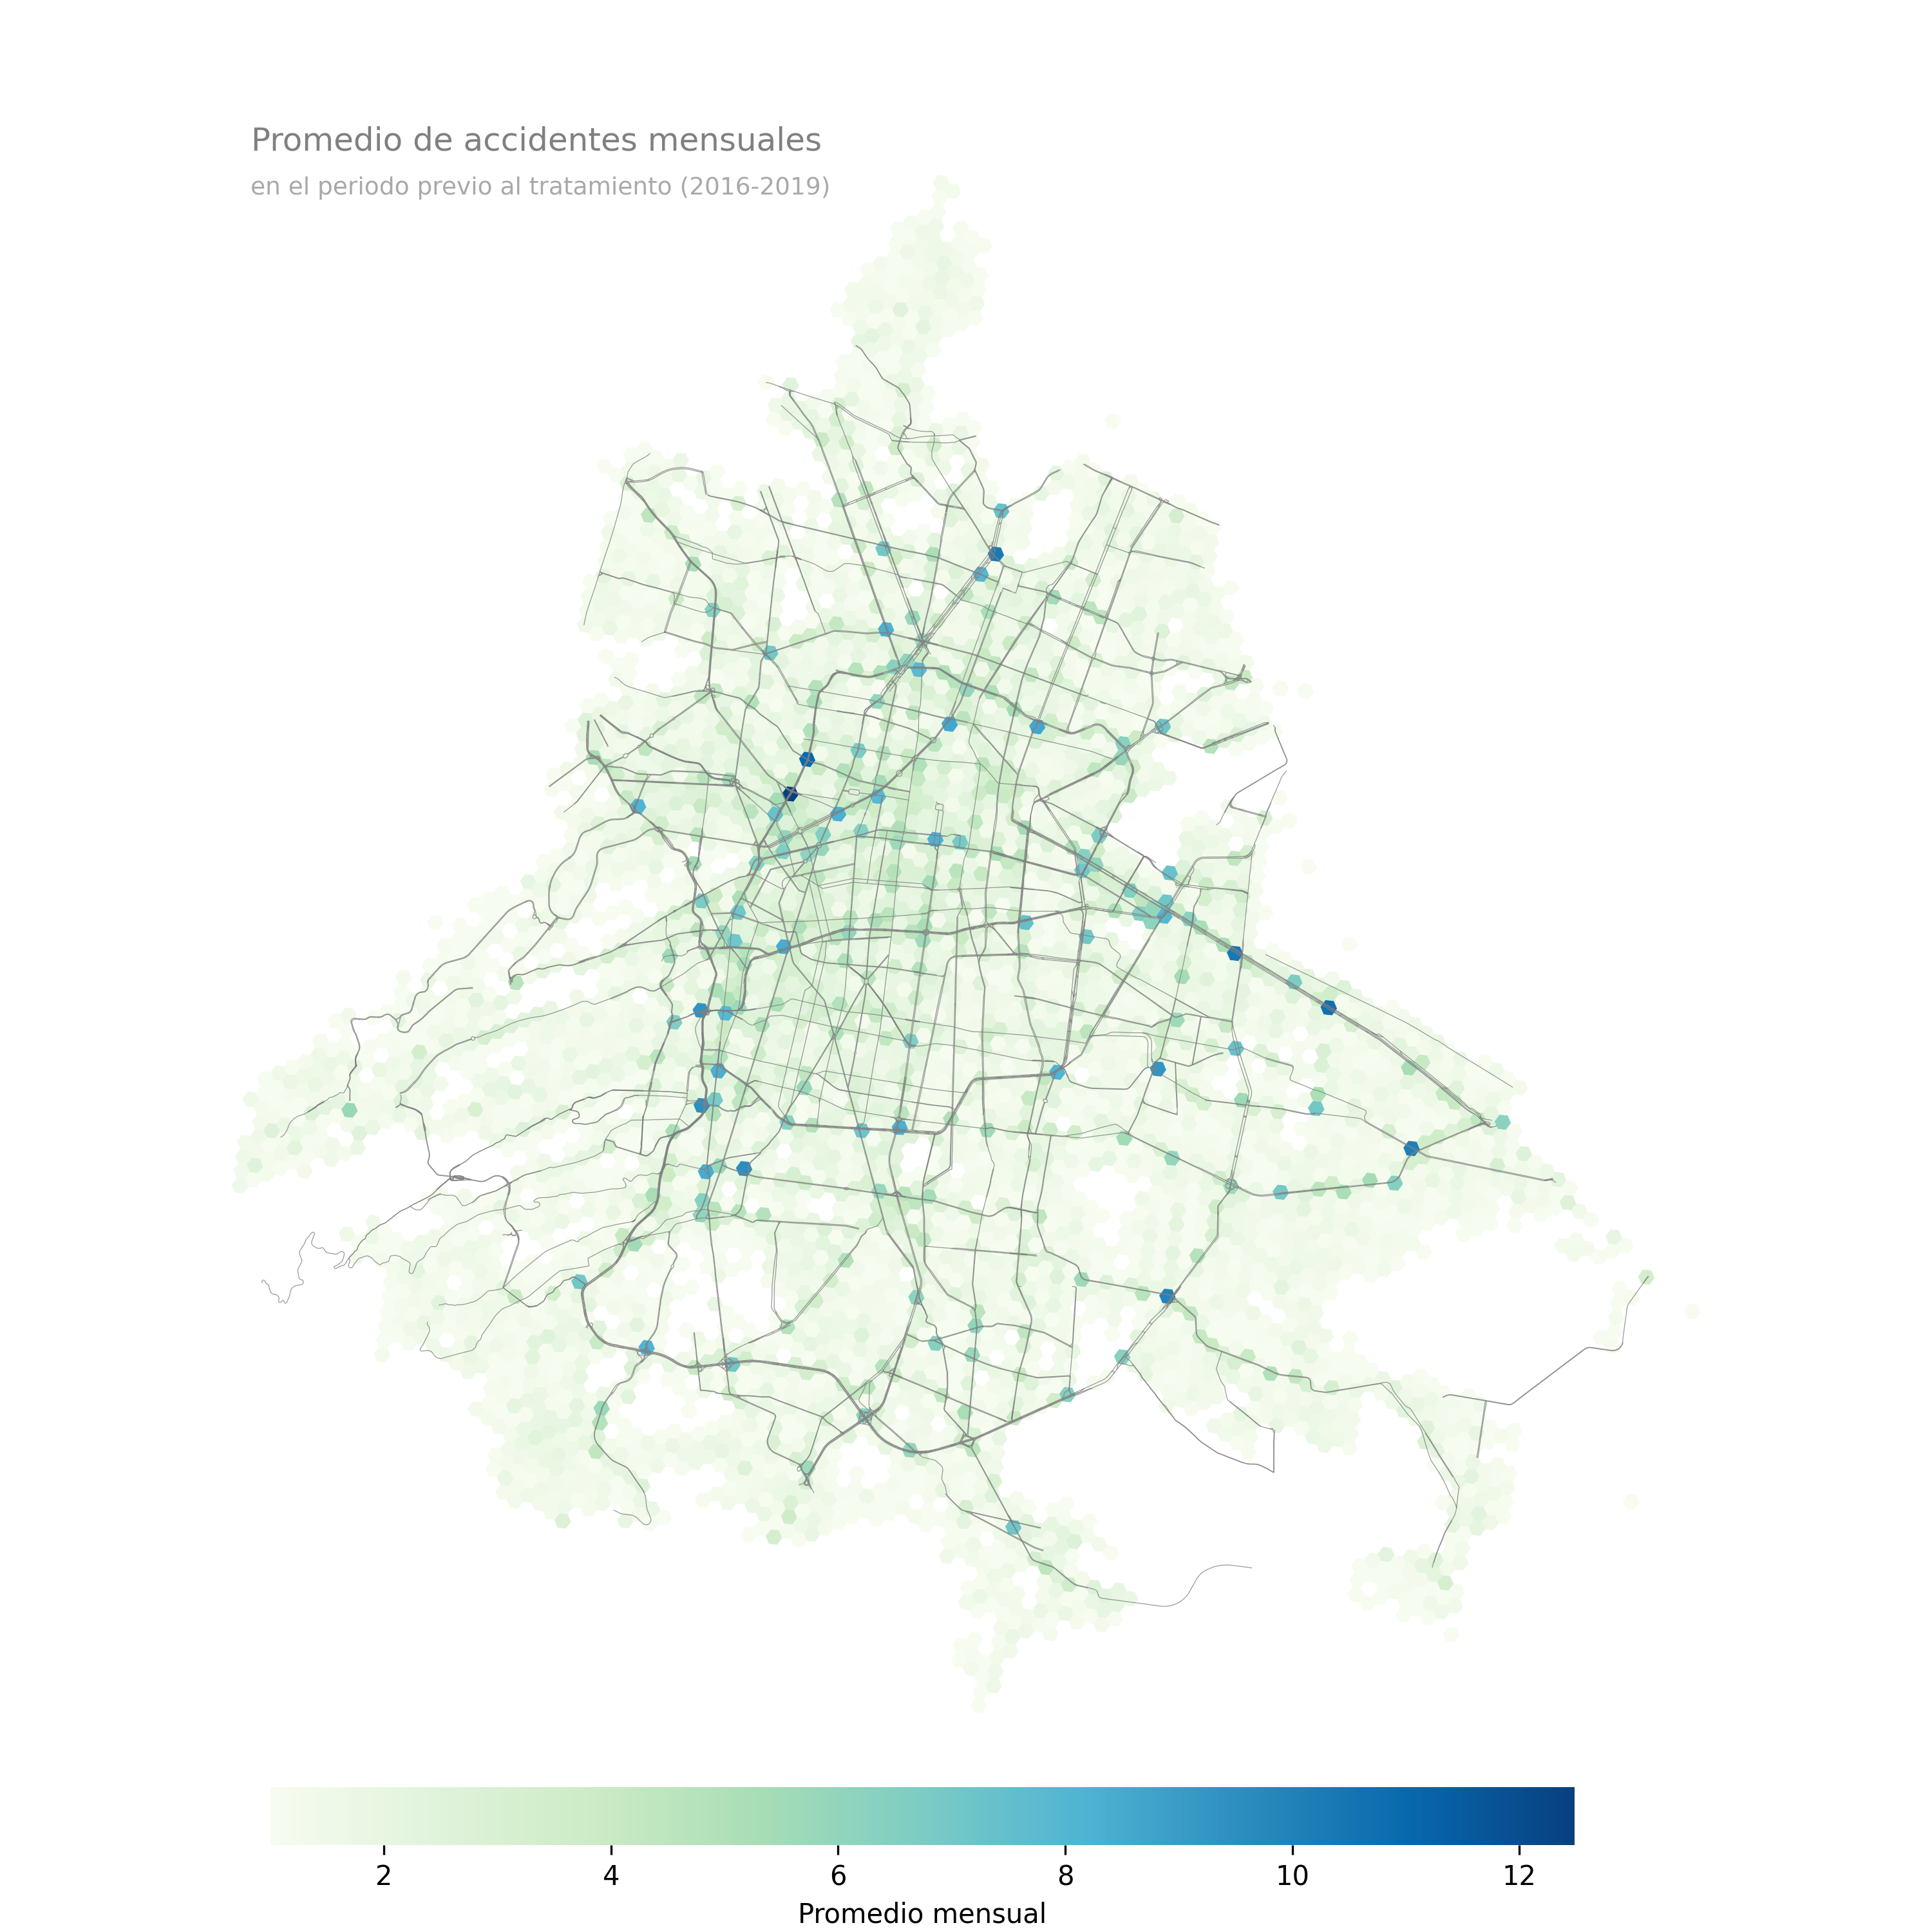
\includegraphics[width=1\linewidth]{Imagenes/promedio-accidenes-mensuales-pre-tratamiento-choroplet.png}
\end{figure}

\begin{figure}
    \centering
    \caption{Distribución de promedio de accidentes mensuales (2016-2019)}
    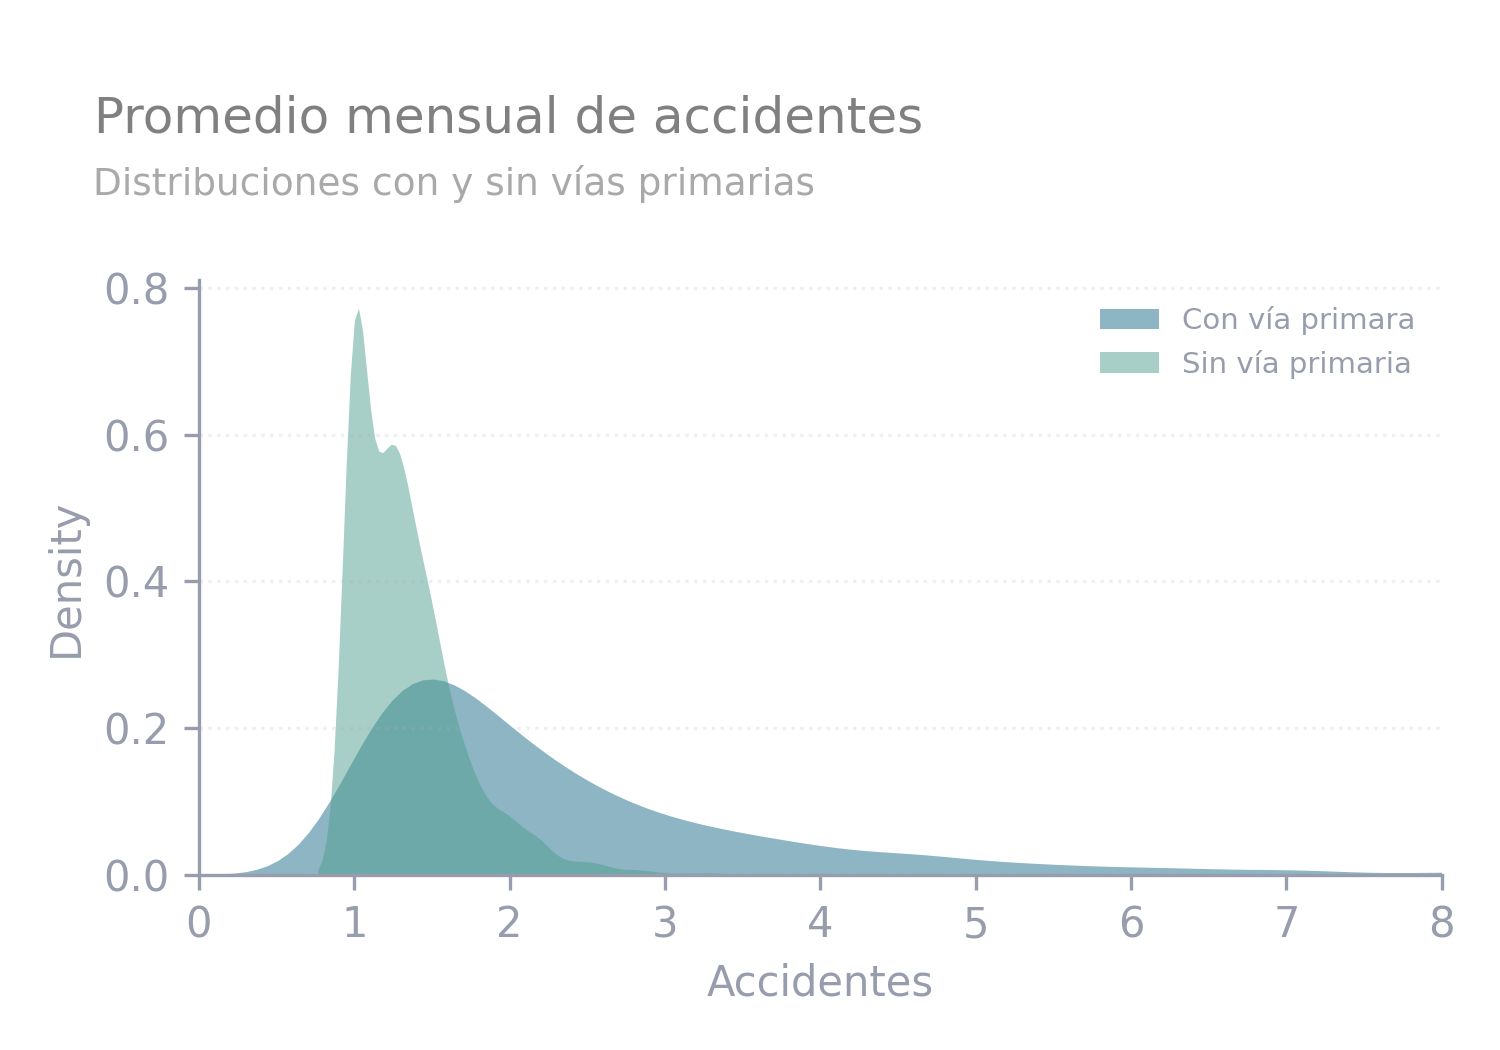
\includegraphics[width=.6\linewidth]{Imagenes/distribucion-promedio-mensual-accidentes-hexagonos.png}
\end{figure}

Por último, las zonas con vías primarias tienden a presentar un perfil de uso de suelo distinto. Para aproximar la intensidad de actividad comercial y de servicios, utilizo la API de \emph{Places Aggregate} de Google para obtener el número de establecimientos por hexágono (de la misma dimensión que el análisis de accidentes). Se diseñó una lista de categorías de lugares que ayudaran a tener una representación general de cada área \footnote{Lista de categorías utilizadas en la llamada a la API de Google Places Aggregate: \texttt{restaurant}, \texttt{cafe}, \texttt{shopping\_mall}, \texttt{supermarket}, \texttt{convenience\_store}, \texttt{grocery\_store}, \texttt{store}, \texttt{gas\_station}, \texttt{bank}, \texttt{atm}, \texttt{hospital}, \texttt{pharmacy}, \texttt{school}, \texttt{gym}, \texttt{night\_club}, \texttt{transit\_station}, \texttt{bus\_station}, \texttt{subway\_station}.}. En promedio, los hexágonos con vías primarias concentran $77.79$ establecimientos (desviación estándar $69.10$), mientras que los hexágonos sin vías primarias tienen en promedio $56.85$ establecimientos (desviación estándar $63.36$). Si bien la variabilidad es alta y la mayor concentración de negocios se observa en torno al centro de la ciudad, existe una diferencia promedio consistente entre ambos tipos de zonas.\\

\begin{figure}
    \centering
    \caption{Distribución de promedio de accidentes mensuales (2016-2019)}
    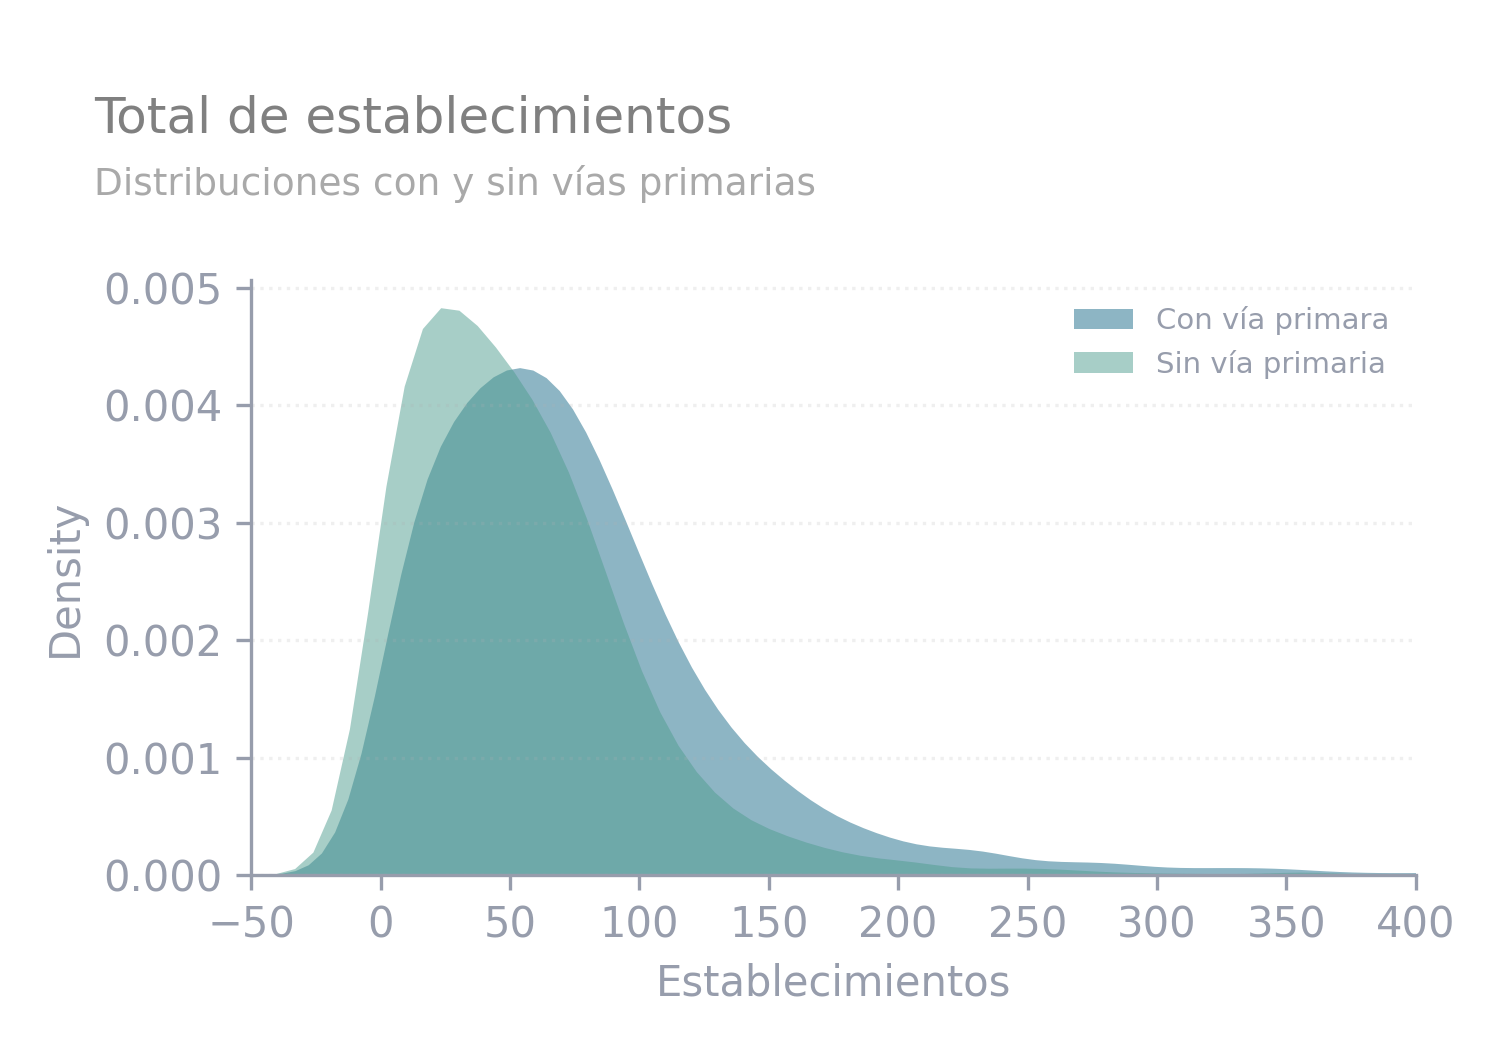
\includegraphics[width=.6\linewidth]{Imagenes/distribucion-establecimientos-cdmx-hexagonos.png}
\end{figure}

\begin{figure}
    \centering
    \caption{Establecimientos en la CDMX}
    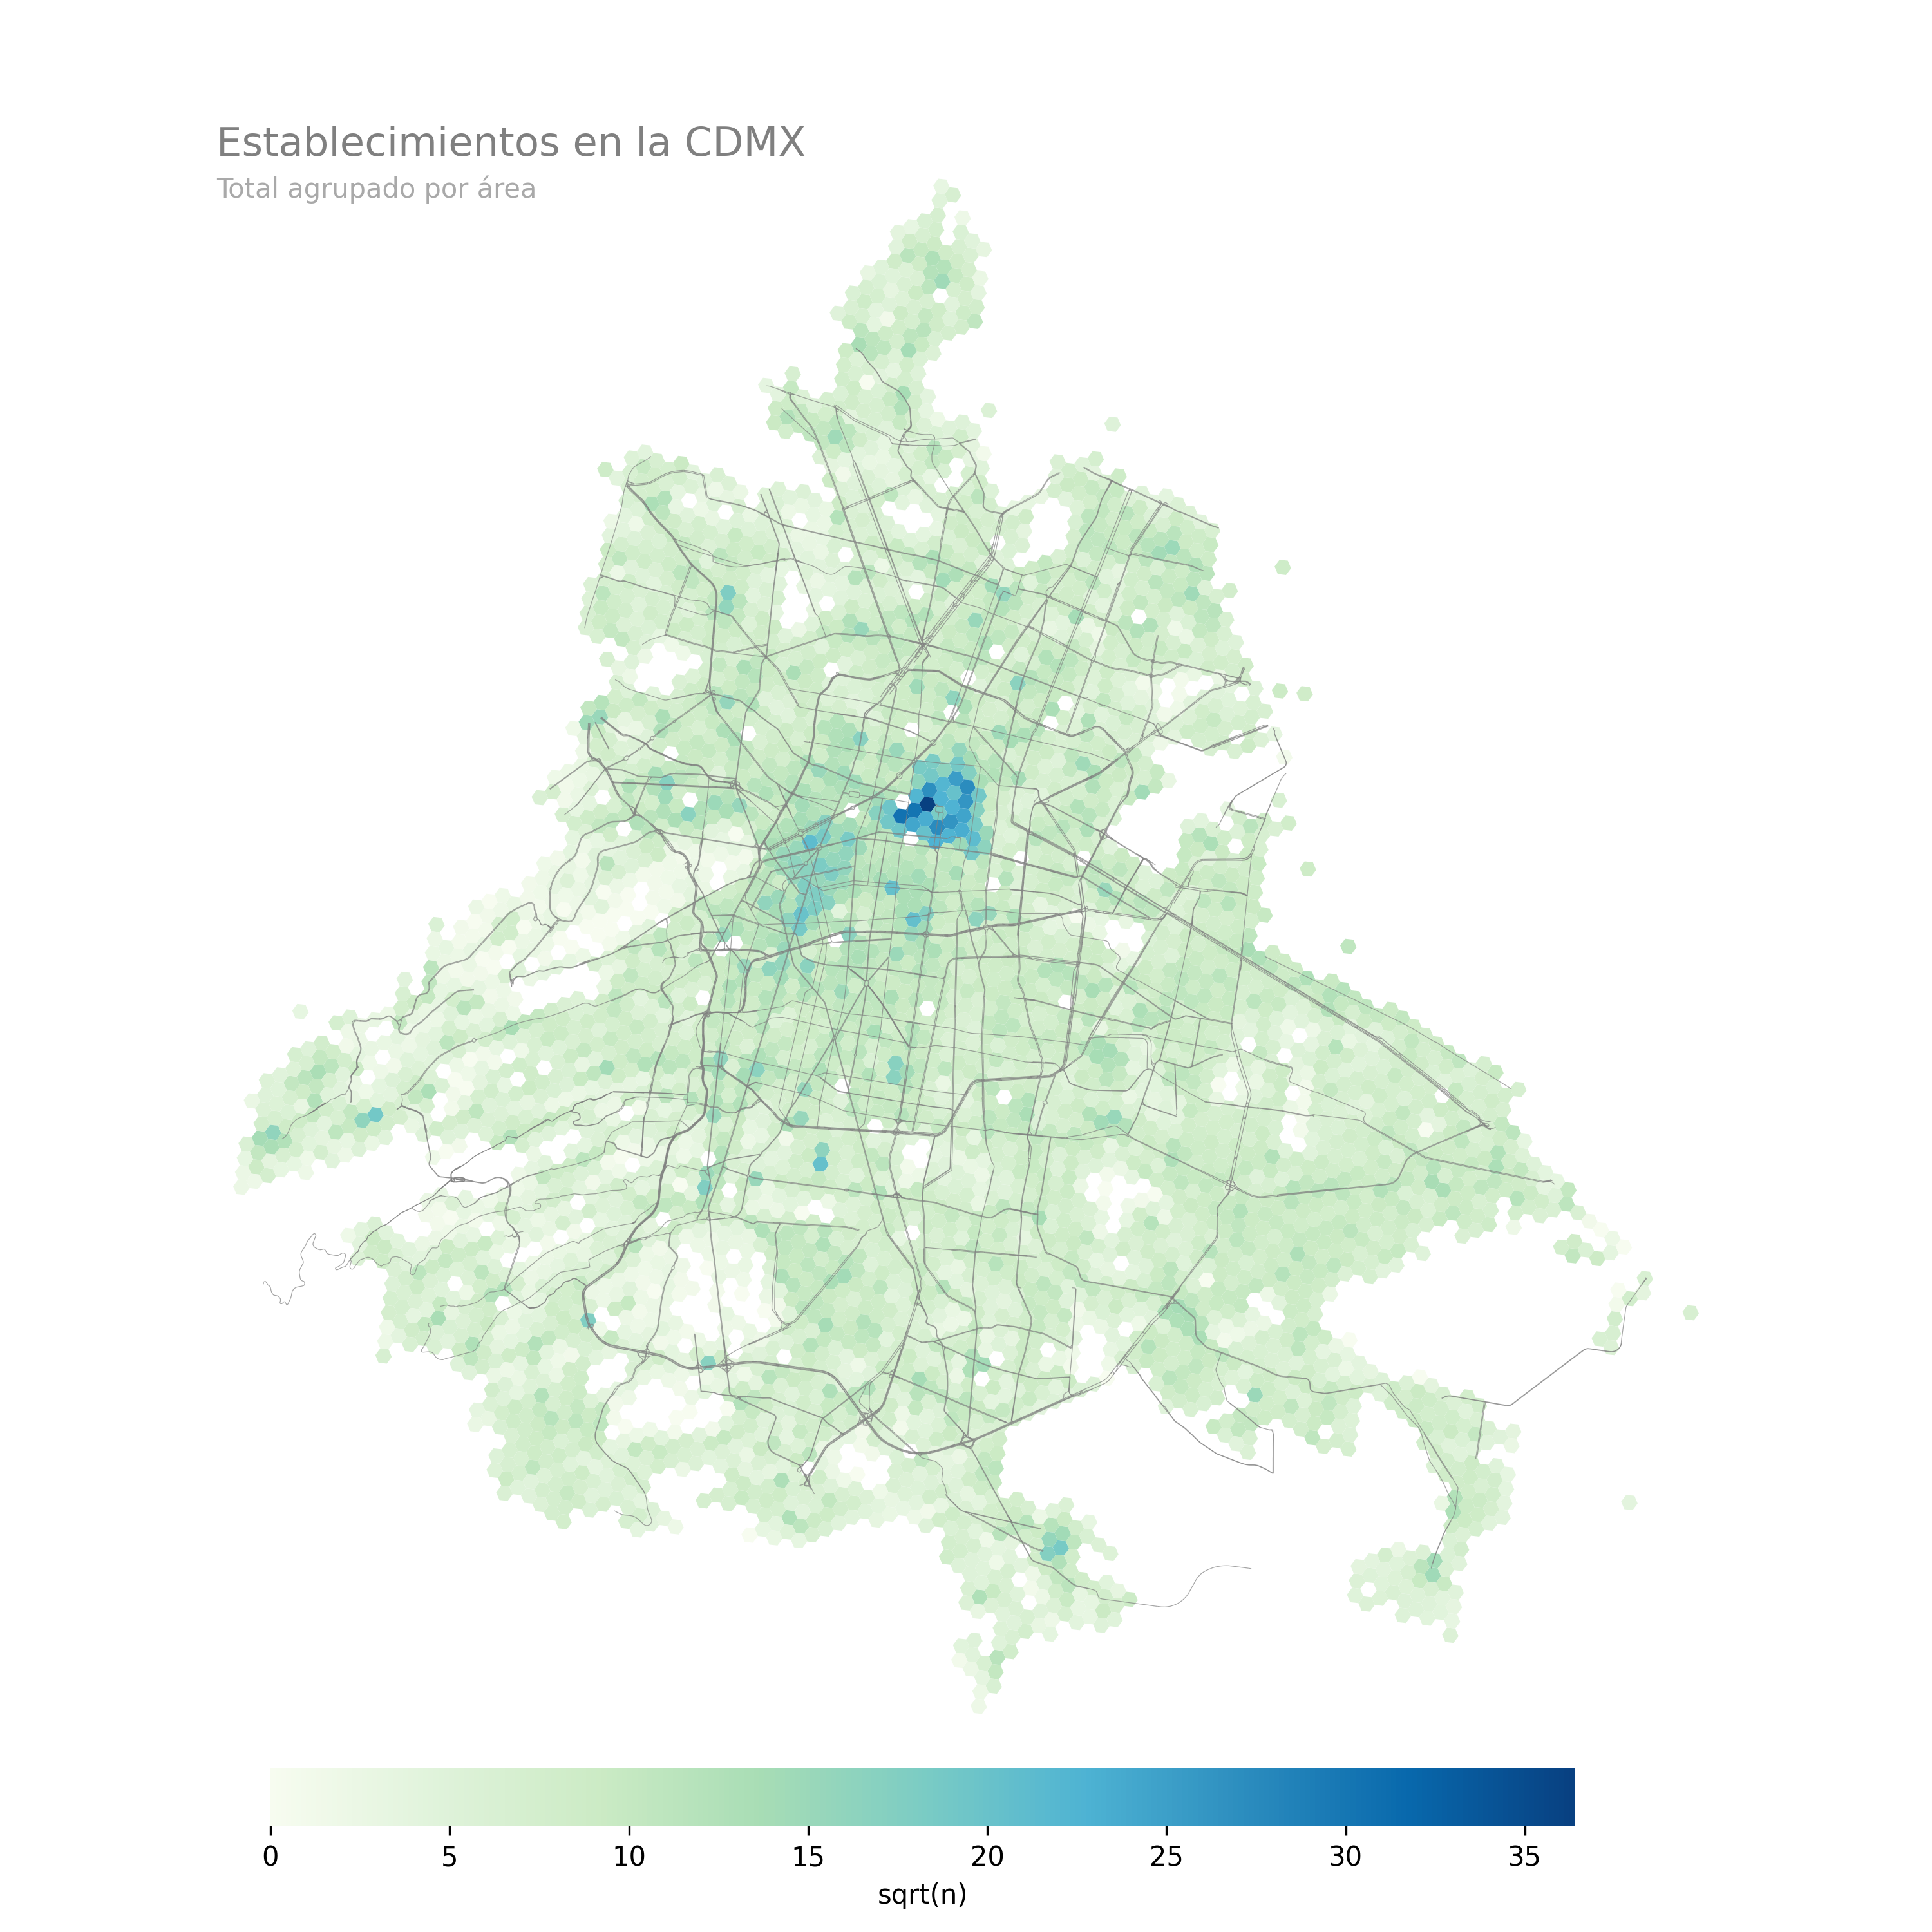
\includegraphics[width=1\linewidth]{Imagenes/establecimientos-en-la-cdmx.png}
\end{figure}
En conjunto, estas diferencias en velocidad reglamentaria, siniestros y nivel de actividad económica muestran que las zonas con y sin vías primarias corresponden a entornos viales y urbanos cualitativamente distintos. Una comparación directa entre ellas introduciría sesgos difíciles de manejar, incluso tras ajustar por covariables observables. Por este motivo, acoto el universo de análisis a las áreas —tratadas y de control— definidas por la malla de círculos alrededor de las cámaras que, además, presentan traslape con al menos una vía primaria de la Ciudad de México. Con base en este universo más homogéneo, en la siguiente sección implemento un procedimiento de emparejamiento por puntaje de propensión, cuyo propósito es hacer más creíbles las comparaciones causales entre áreas tratadas y de control.

\section{Estrategia de identificación}
\noindent El objetivo de esta tesis es estimar el efecto causal de la instalación de cámaras de velocidad sobre la seguridad vial en su entorno inmediato. En particular, me interesa cuantificar cómo cambia, en las áreas donde se colocaron radares, el promedio mensual de accidentes por nivel de severidad y la tasa promedio mensual de accidentes, en comparación con lo que hubiera ocurrido en ausencia de cámaras. En términos de inferencia causal, este efecto se interpreta como un \emph{average treatment effect on the treated} (ATT): el efecto promedio de contar con cámara sobre las áreas efectivamente tratadas, tomando como contrafactual áreas de control emparejadas que comparten características observables similares.\\

Dada la naturaleza panel de la base de datos y el hecho de que el programa de fotocívicas se implementó simultáneamente para todas las cámaras el 22 de abril de 2019, la estrategia principal de estimación se basa en modelos de diferencia en diferencias con efectos fijos. La unidad de observación es el área de análisis (círculo tratado o de control) en cada periodo, y el modelo incluye efectos fijos por unidad y por mes, de modo que se controlan tanto las características invariables en el tiempo de cada área como los choques comunes a toda la ciudad en cada periodo. El coeficiente de interés es el de la interacción entre una dummy de tratamiento (área con cámara) y una dummy de periodo posterior a la entrada en vigor del programa; este parámetro captura el cambio diferencial en los resultados de seguridad vial en áreas tratadas frente a sus controles después de la instalación de las cámaras.\\

Existen, en principio, varias formas alternativas de aproximarse a este problema. Una opción natural sería un ejercicio tipo \emph{before--after} en las áreas donde se instalaron las cámaras, comparando directamente el nivel de siniestros antes y después de abril de 2019. Sin embargo, esta aproximación es especialmente problemática en este contexto por dos razones. Primero, el periodo de estudio incluye el choque exógeno de la pandemia de COVID-19, que alteró de manera drástica los patrones de movilidad y, por tanto, la siniestralidad vial. Un simple \emph{before--after} confundiría los efectos de la pandemia con los del programa de fotocívicas. Segundo, incluso en ausencia de la pandemia, cualquier cambio en tendencias generales de accidentes en la ciudad podría ser erróneamente atribuido a las cámaras si no se cuenta con un grupo de comparación adecuado.\\

Otra alternativa sería estimar un modelo de diferencia en diferencias utilizando como controles todas las áreas elegibles que no recibieron cámaras. Sin embargo, como se discutió en la sección anterior, la asignación del programa no fue aleatoria: por diseño, las cámaras se instalaron en zonas con mayor riesgo vial. Usar de manera indiscriminada todas las demás áreas como contrafactual heredaría este sesgo de selección y llevaría a comparar zonas sistemáticamente más peligrosas con otras estructuralmente distintas, incluso si se controla por algunas covariables en la regresión. Bajo estas condiciones, el supuesto de independencia condicional resulta poco creíble.\\

También es conceptualmente posible apoyarse únicamente en \emph{propensity score matching} (PSM), emparejando cada área tratada con una o varias áreas de control similares en sus covariables pretratamiento y estimando el efecto como el promedio de las diferencias en los resultados. No obstante, el tratamiento aquí no es un evento puntual observado una sola vez, sino una intervención permanente a partir de una fecha concreta. En este marco, la estructura temporal contiene información valiosa que se desperdiciaría si se redujera el análisis a un comparativo estático entre tratadas y controles. Por ello, resulta más natural combinar el emparejamiento con un modelo de diferencia en diferencias.\\

En esta tesis, la estrategia de identificación combina precisamente ambas herramientas: primero, utilizo el \emph{propensity score} para construir pares de áreas tratadas y de control que sean lo más comparables posible en términos de covariables observables; después, aplico sobre esta muestra emparejada una regresión de diferencia en diferencias con efectos fijos por unidad y por mes. De esta manera, el \emph{matching} actúa como un paso de preprocesamiento que mejora la calidad del grupo de comparación, mientras que la estructura panel permite aislar cambios diferenciales en el tiempo asociados a la implementación del programa.\\

La probabilidad que se modela en el paso de PSM es la probabilidad de que un área determinada cuente con una cámara de velocidad condicional en las covariables observables seleccionadas. Para ello, estimo un modelo logístico en el que la variable dependiente es una dummy de tratamiento (presencia de cámara) y los regresores incluyen las características del entorno vial y urbano disponibles en el periodo pretratamiento. El \emph{propensity score} resume así, en una sola dimensión, la información relevante de las covariables utilizadas para la asignación del programa.\\

A partir de estos puntajes de propensión, implemento un esquema de \emph{nearest neighbor matching} 1:1 sin reemplazo. Es decir, para cada área tratada se selecciona como control aquella área sin cámara cuyo \emph{propensity score} presenta la menor diferencia absoluta respecto al de la unidad tratada, y cada área de control se utiliza a lo más una vez. Opto por el emparejamiento 1:1 sin reemplazo por dos motivos. Primero, garantiza que cada unidad de control emparejada representa un contrafactual razonablemente cercano en términos de probabilidad de tratamiento, en lugar de reutilizar en exceso un pequeño conjunto de controles “muy buenos”, lo que concentraría la inferencia en pocas zonas de la ciudad. Segundo, en las pruebas de balance, esta configuración produjo la mejor combinación entre similitud de covariables y tamaño efectivo de la muestra: al intentar emparejar más de un control por tratada se incrementaba el ruido, pues necesariamente se incorporaban pares con diferencias más grandes en el \emph{propensity score}.\\

Un requisito central de esta estrategia es el supuesto de \emph{common support}: para cada valor del \emph{propensity score} observado en las áreas tratadas debe existir un conjunto suficiente de áreas de control con valores similares. Más adelante, en la sección de balance, muestro la distribución de los puntajes de propensión para unidades tratadas y de control y verifico que, en términos generales, existe un traslape amplio entre ambos grupos. No obstante, en algunos radios fue necesario restringir la muestra y excluir ciertas áreas tratadas ubicadas en zonas del puntaje de propensión con muy poca densidad de controles comparables. Este recorte permite que el emparejamiento se realice únicamente en la región donde la comparación entre tratadas y controles resulta defendible.\\

La calidad del emparejamiento se evalúa mediante la \emph{standardized mean difference} (SMD) para cada covariable incluida en el modelo de \emph{propensity score}. Reporto los valores de SMD antes y después del \emph{matching} y utilizo como referencia el criterio usual de considerar aceptable un desbalance inferior a 0.1 en valor absoluto. Si bien no todas las covariables alcanzan exactamente ese umbral, los desbalances residuales son pequeños y se reducen de manera sustancial respecto a la muestra original. Esto indica que, después del emparejamiento, las distribuciones de las covariables observables en los grupos tratado y de control son muy similares.\\

Una vez construido el conjunto de pares tratada–control, estimo el efecto de las cámaras mediante una regresión de diferencia en diferencias, utilizando como unidades tratadas las áreas con radares de velocidad y como controles sus respectivos \emph{matches}. Dado que el emparejamiento ya garantiza un alto grado de similitud en las covariables observables pretratamiento, especifico el modelo de diferencia en diferencias únicamente con efectos fijos por unidad y por mes, sin añadir controles adicionales. La inclusión de efectos fijos por área captura diferencias invariables en el tiempo entre cada par tratada–control, mientras que los efectos fijos temporales recogen shocks comunes (incluido el choque de la pandemia) que afectan de manera similar a todas las áreas en un mismo periodo. Bajo el supuesto estándar de tendencias paralelas entre los grupos emparejados, el coeficiente de la interacción tratamiento–periodo posterior puede interpretarse como el efecto causal promedio de las cámaras sobre los resultados de seguridad vial en las áreas tratadas.\\

Esta combinación también vuelve más creíble la comparación entre áreas tratadas y de control. Dado que las cámaras se reubicaron hacia zonas con mayor riesgo, no basta con comparar cualquier vialidad con cámara contra cualquier vialidad sin cámara. El emparejamiento permite partir de áreas observacionalmente similares, y la diferencia en diferencias aprovecha esa base para aislar mejor los cambios posteriores a la implementación del programa.

\noindent A partir de esta discusión conceptual, en esta sección presento la evidencia empírica que utilizo para evaluar qué tan aceptable es ese supuesto en la muestra emparejada. La verificación se apoya en dos pruebas complementarias. La primera es una inspección visual de las trayectorias pevias al tratamiento. Para ello, construyo gráficas de tendencias mensuales promedio para los distintos radios evaluados, comparando en cada caso las áreas tratadas con: (i) todos los controles elegibles y (ii) los controles emparejados por \emph{propensity score}. Hago uso de tres años de información previos a la implementación y tres años posteriores, y se realiza para el total de accidentes y para cada nivel de severidad (\emph{MIN}, \emph{PIC} y \emph{FCS}). En la muestra sin emparejar, las áreas tratadas presentan de manera sistemática niveles promedio de siniestralidad más altos, algo consistente con el sesgo de selección que motivó el uso de PSM. Aun así, en términos generales las trayectorias previas ya lucen parecidas. Después del emparejamiento, el traslape entre curvas aumenta de forma importante: no solo se reducen las diferencias de nivel, sino que las tendencias se vuelven mucho más similares. Las series de accidentes fatales son más ruidosas, algo esperable dada la baja frecuencia de estos eventos. El caso donde todavía se aprecia una diferencia más visible es el de accidentes menores en el radio de 50 metros, donde alrededor de año y medio antes de la intervención persiste una ligera discrepancia; aun así, esa diferencia es menor que la observada en la muestra original. La figura siguiente muestra precisamente ese radio.\\

\begin{figure}[htbp]
    \centering
    \caption{Tendencias promedio mensuales de accidentes en radios de 50 metros, con y sin matching}
    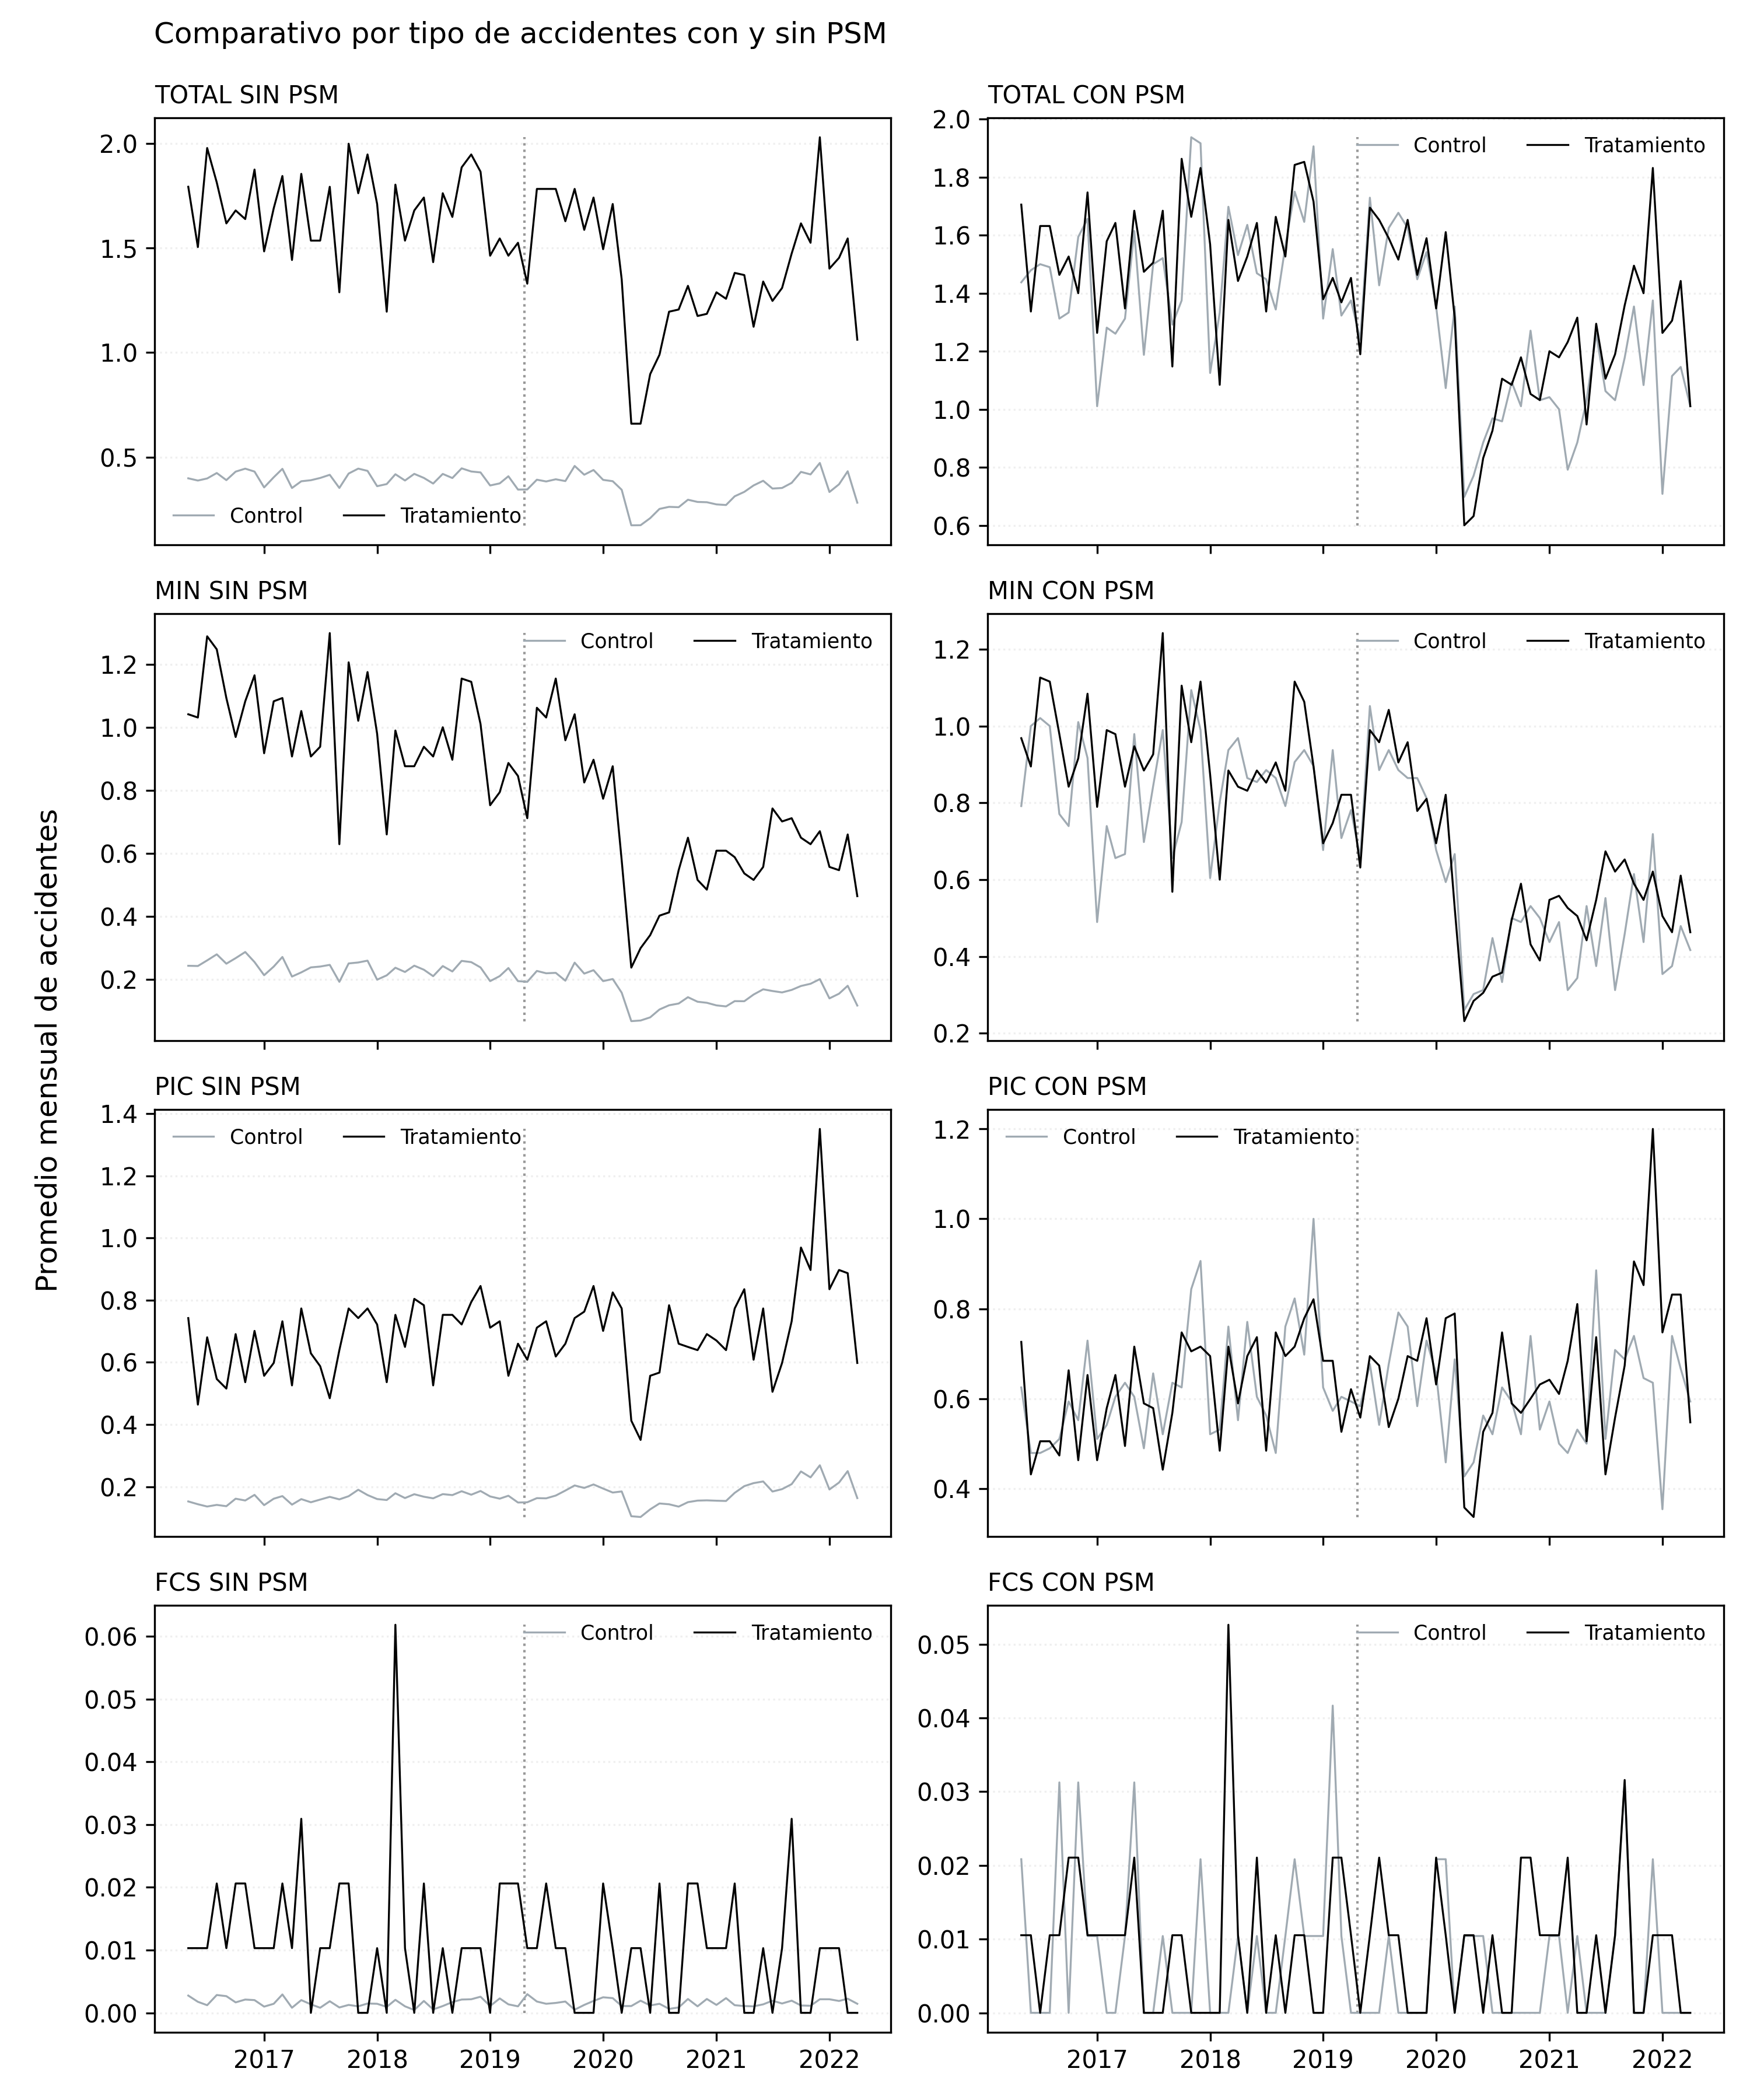
\includegraphics[width=\textwidth]{Imagenes/mean_accidents_trends/trend_mean_accidents_50.png}
\end{figure}

La segunda evaluación consiste en pruebas placebo usando exclusivamente los tres años previos al inicio del programa. Para ello, vuelvo a estimar la especificación principal sobre la misma muestra emparejada, pero asignando fechas ficticias de tratamiento a 18, 12 y 6 meses antes de la implementación real. Lo que esperaríamos es lo siguiente: si el modelo estuviera detectando diferencias previas entre tratados y controles, deberían aparecer coeficientes significativos incluso antes de que el programa comenzara. En total, se estiman 144 coeficientes para los distintos radios, variables de resultado y ventanas placebo. De ellos, 143 no son estadísticamente significativos. La única excepción aparece en la tasa de accidentes menores para el radio de 50 metros cuando la fecha de prueba se ubica 18 meses antes del inicio del programa, con significancia al 95\%. Estos resultados son consistentes con el supuesto de tendencias paralelas, aunque sugieren interpretar con un poco más de cautela esa especificación puntual.\\

La evidencia presentada no permite probar de forma definitiva el supuesto de tendencias paralelas, algo que además no es posible hacer de manera directa. Sin embargo, sí aporta elementos a favor de su plausibilidad. En especial, una vez construido el grupo de control mediante \emph{propensity score matching}, las áreas tratadas y sus controles emparejados muestran trayectorias antes del tratamiento que son similares y, salvo una excepción aislada, no presentan efectos placebo previos a la implementación del programa. En este sentido, la evidencia respalda la interpretación del coeficiente de diferencia en diferencias como una aproximación al efecto causal de las cámaras sobre la siniestralidad vial.\\

Finalmente, una ventaja adicional de esta estrategia es su interpretabilidad y capacidad de replicación. Al partir de una comparación explícita entre áreas tratadas y controles muy similares, y estimar un efecto promedio bien definido sobre las unidades tratadas, los resultados pueden traducirse directamente en recomendaciones de política. En particular, si se encuentra que las cámaras reducen de manera significativa la frecuencia o la severidad de los accidentes en su entorno inmediato, el mismo procedimiento de emparejamiento puede utilizarse en una segunda etapa para identificar qué otras áreas de la ciudad presentan perfiles de riesgo y características viales similares a las zonas tratadas actuales. Estas áreas serían candidatas naturales para una eventual expansión del programa de fotocívicas, manteniendo la lógica de focalizar la intervención donde los beneficios esperados sean mayores.\\ 


\chapter{Datos y balance}

\noindent Para que el análisis del impacto del programa de fotocívicas en la seguridad vial de la Ciudad de México sea factible y estadísticamente robusto, es necesario integrar diversos conjuntos de datos abiertos, organizados en tres categorías fundamentales para la inferencia causal: \textit{treatment}, \textit{outcomes} y \textit{covariates}. El tratamiento se define a partir de la ubicación geográfica de los 113 radares de velocidad registrados por la Secretaría de Seguridad Ciudadana (SSC), lo que permite identificar de manera explícita las unidades espaciales intervenidas por la política. En cuanto a los resultados (\textit{outcomes}), estos corresponden a los incidentes viales confirmados en los registros del C5, analizados tanto en números absolutos como en tasas por cada 1{,}000 vehículos. Esta construcción posibilita una desagregación por nivel de severidad, distinguiendo entre incidentes menores (MIN), con lesiones personales (PIC) y aquellos con víctimas fatales (FCS).\\

Las covariables (\textit{covariates}) cumplen un papel central en el control de los factores que influyen en la asignación de las cámaras y en la garantía de comparabilidad entre unidades mediante el cálculo del \textit{propensity score}. Para ello, se consideran atributos estáticos, que describen la configuración física e invariable de la red vial (jerarquía, número de carriles, sentido y nivel de la traza), así como variables que cambian en el tiempo, empleadas como \textit{proxies} de movilidad para capturar las variaciones en la exposición vehicular asociadas a la pandemia de COVID-19. En particular, la integración de la afluencia diaria del Metro y los volúmenes de tránsito mensual reportados por la SICT contribuye a mitigar sesgos derivados de choques exógenos, y sienta las bases para la implementación de un diseño de diferencias en diferencias aplicado sobre una muestra emparejada con soporte común.

\section{Tratamiento: Programa de Fotocívicas}
El objetivo central de este análisis es identificar el efecto causal de las cámaras de velocidad sobre el número de incidentes viales en la Ciudad de México. Para ello, resulta indispensable contar con la ubicación geográfica precisa de los radares, ya que estos puntos determinan la delimitación de las áreas consideradas como unidades tratadas y sirven como base para la construcción de las unidades de control en el modelo de emparejamiento. A diferencia del esquema previo de fotomultas, la ubicación de estos dispositivos es de acceso público, decisión que se alinea con la naturaleza preventiva del programa de fotocívicas, vigente desde el 22 de abril de 2019. Esta transparencia busca propiciar un cambio genuino en las conductas de los conductores al incentivar el respeto a los límites de velocidad mediante la localización explícita de los equipos, privilegiando la educación vial por encima de la recaudación económica.\\

De acuerdo con los registros de la Secretaría de Seguridad Ciudadana (SSC), el tratamiento se define a partir de un total de 113 radares de velocidad distribuidos en las principales vialidades de la ciudad. La información se obtiene del conjunto de datos \textit{``Fotocívicas (Ubicación)''}, publicado en la Plataforma de Datos Abiertos de la Ciudad de México y actualizado por última vez el 6 de julio de 2023. Este conjunto proporciona variables clave para el análisis geoespacial, entre ellas el nombre de la vialidad, el sentido de circulación sobre el cual opera la cámara y sus coordenadas exactas (latitud y longitud). A partir de estos insumos se define operativamente la variable binaria \texttt{has\_camera} a nivel de celda o área circular, lo que permite identificar la exposición espacial al tratamiento y sienta las bases para la posterior implementación del diseño de diferencia en diferencias.

% aquí está pendiente además mostrar cómo se ve un ejemplo concreto de una unidad tratada y la construcción de sus controles aledaños para que la gente pueda entender a qué es a lo que me estoy refiriendo. También falta detallar que has camera es una variable binaria con valores 0 y 1, para cuando no tienen cámara de velocidad y cuando sí la tienen respectivamete. 

\section{Covariables Geográficas, Estructurales y de Movilidad}
Para mitigar el sesgo de selección inherente al programa de Fotocívicas -- donde los radares se ubican estratégicamente en tramos con mayor siniestralidad, altos volúmenes de traslado y recurrente incumplimiento de límites de velocidad -- es necesario controlar por las características estructurales de la vía. A continuación se describen las covariables de los atributos físicos de la red vial, construidas a partir del conjunto de datos \textit{Vialidades primarias de la Ciudad de México} proporcionado por la Secretaría de Movilidad (SEMOVI). 

\subsubsection{Atributos físicos de la red vial}

\begin{itemize}
    \item \textbf{Número de vialidades (\textit{n\_vialidades}):} 
    Esta variable contabiliza el número de ejes viales únicos que intersectan cada unidad de análisis. Permite controlar por la densidad de la red y la complejidad de la conectividad local, factores que elevan la probabilidad de conflictos vehiculares y, por ende, la probabilidad de que la autoridad asigne una cámara en dicho punto.

    \item \textbf{Capacidad de la vía (\textit{max\_carriles}):} 
    Corresponde al número máximo de carriles observado entre las vialidades de la celda. Se utiliza como un proxy de la capacidad vial y del volumen potencial de tránsito. Las vías con mayor número de carriles suelen permitir velocidades más altas y concentrar flujos masivos, lo que las hace candidatas prioritarias para el tratamiento.

    \item \textbf{Sentido de circulación (\textit{both\_directions}):} 
    Indicador binario que señala la presencia de al menos una vialidad de doble sentido en el área. La direccionalidad influye en la siniestralidad al introducir maniobras de giro y potenciales conflictos frontales o laterales que no existen en vías de un solo sentido.

    \item \textbf{Jerarquía vial (\textit{via\_primaria}):} 
    Variable dicotómica que indica si la unidad contiene vías clasificadas como primarias. Según el Reglamento de Tránsito, estas vías tienen funciones de flujo continuo o controlado por semáforos y límites de velocidad específicos (50 km/h), lo que las define como el objetivo central del programa sancionatorio.

    \item \textbf{Vías de acceso controlado (\textit{via\_acc\_cont}):} 
    Identifica la presencia de corredores con regulación y geometría específica, como entradas y salidas mediante carriles de aceleración y desincorporación. Estas vías (con límites de hasta 80 km/h) presentan niveles de riesgo y exposición distintos a las arterias convencionales, influyendo directamente en la decisión gubernamental de monitoreo.

    \item \textbf{Complejidad vertical (\textit{max\_nivel}):} 
    Representa el nivel máximo sobre el suelo (\textit{z-order}) de las vialidades presentes. Esta covariable es crítica en la Ciudad de México para encapsular la dinámica de vías de múltiples niveles, como el segundo piso del Periférico, donde los riesgos de siniestralidad y la visibilidad de los radares difieren del nivel de calle.

    \item \textbf{Longitud vial acumulada (\textit{road\_length\_m}):} 
    Mide la cantidad total de metros de red vial contenidos dentro del área de estudio. El control por longitud permite realizar un emparejamiento basado en la exposición física: una alta concentración de metros de vía suele corresponder a cruces de grandes avenidas o nudos viales complejos, los cuales implican un mayor flujo vehicular y una probabilidad intrínsecamente más alta de colisiones.
\end{itemize}

Estas variables operan como controles fijos en el cálculo del \textit{propensity score}, garantizando que la comparación se realice entre tramos viales con estructuras físicas, capacidades y jerarquías comparables, aislando así el efecto del radar de la peligrosidad natural del diseño vial.

\subsubsection{Proxies de movilidad y exposición}

Para capturar la dinámica de movilidad urbana y mitigar las distorsiones causadas por cambios en el flujo de personas, especialmente ante choques exógenos, se incorporaron \textit{proxies de movilidad} basados en el sistema de transporte masivo de la ciudad. El uso de estos indicadores es fundamental para controlar el choque exógeno de la pandemia de COVID-19, la cual provocó una reducción en la movilidad de entre el 40\% y el 60\%, permitiendo velocidades de circulación más altas y una recomposición en la severidad de los incidentes viales. A continuación se detalla la construcción y el procesamiento de estas fuentes.

\paragraph{Fuentes de datos}

\begin{itemize}
    \item \textbf{Coordenadas de estaciones de metro (\textit{metro coordinates}):} 
    Ante la ausencia de un registro unificado con precisión geográfica para todas las estaciones, se generó un conjunto de datos de creación propia mediante la extracción automática de información de Google Maps. Este proceso consistió en la búsqueda sistemática de cada una de las 167 estaciones del sistema para registrar sus coordenadas geográficas exactas (latitud y longitud), permitiendo así la georreferenciación precisa de la infraestructura de transporte dentro de la cuadrícula de análisis.

    \item \textbf{Afluencia del metro:} 
    Se utilizó el conjunto de datos \textit{``Afluencia diaria del metro CDMX''}, proporcionado por la Secretaría de Movilidad (SEMOVI), el cual registra el volumen diario de usuarios por línea y estación. Estos datos, con cobertura desde enero de 2010 hasta abril de 2025, se unieron (\textit{join}) con las coordenadas geográficas previamente obtenidas para localizar los flujos de personas en el espacio urbano.
\end{itemize}

\subsubsection{Construcción de variables para el emparejamiento (\textit{matching})}

Para que estos datos temporales pudieran integrarse en el cálculo del \textit{propensity score} y asegurar que las unidades tratadas y de control fueran comparables en su dinámica de flujo previa a la intervención, se aplicó un proceso de agregación y ``compresión'' de las series históricas. A cada unidad de análisis (celda) se le asignó la información de la estación de metro más cercana, asumiendo que esta es la representación más fiel del flujo humano y la actividad comercial en esa zona específica.

Las variables resultantes para el \textit{matching}, calculadas exclusivamente con datos previos al inicio del programa (22 de abril de 2019), son las siguientes:

\begin{itemize}
    \item \textbf{Distancia a la estación (\textit{distance\_to\_station}):} 
    Mide la distancia en metros desde el centroide de cada celda a la estación de metro más cercana, sirviendo como un control de proximidad a nodos de alta actividad.

    \item \textbf{Media de afluencia mensual (\textit{mean\_afluencia\_mensual}):} 
    Representa el nivel promedio de demanda y exposición peatonal/vehicular de la zona durante el periodo preintervención.

    \item \textbf{Desviación estándar de la afluencia (\textit{std\_afluencia\_mensual}):} 
    Captura la volatilidad o variabilidad de los flujos en la zona, permitiendo emparejar celdas que no solo comparten niveles de tráfico similares, sino también patrones de estabilidad o fluctuación parecidos.
\end{itemize}

Este tratamiento de los datos permite que el modelo de evaluación asuma que, tras el emparejamiento, las diferencias en la siniestralidad no son producto de variaciones locales en la movilidad o del impacto diferenciado de la pandemia, sino del efecto causal de los radares de velocidad.

\subsubsection{Estaciones de conteo permanente de tránsito}

Para captar la exposición vehicular y el volumen de tráfico —factores que con frecuencia se omiten en evaluaciones locales de seguridad vial— incorporo datos de las \textit{estaciones de conteo permanente} mantenidas por la Secretaría de Infraestructura, Comunicaciones y Transportes (SICT).

\paragraph{Obtención y procesamiento de los datos}

La información se extrajo de los informes anuales de \textit{Datos Viales} (con cobertura de 2015 a 2024), los cuales reportan el volumen total anual y la distribución porcentual mensual para distintos puntos de la red carretera. Dado que estos datos se publican en archivos PDF no estructurados y con identificadores inconsistentes, fue necesario desarrollar una metodología de procesamiento que garantizara la integridad de la información. 

Este proceso incluyó la localización de las tablas relevantes a partir de coordenadas geográficas y tramos carreteros, el uso de un \textit{large language model} (LLM) para extraer las cifras a un formato estructurado y la validación manual para seleccionar las 20 estaciones que permanecieron operando de manera continua durante todo el periodo de análisis.

\paragraph{Contribución a la literatura}

El uso de estas series representa una contribución importante a la literatura de seguridad vial en la Ciudad de México. Estudios previos —como Quintero et al.\ (2022) o Madrigal y Rodríguez (2021)— no utilizaron estos conjuntos de datos específicos de la SICT para controlar el choque exógeno de la pandemia de COVID-19 ni las variaciones generales en la exposición. Al integrar estas cifras, el presente estudio incorpora un control más robusto para las caídas abruptas en el tráfico (estimadas entre 40\% y 60\% durante 2020) que, de otra forma, sesgarían la estimación del impacto de los radares de velocidad.

\paragraph{Resolución espacial y estandarización}

Una limitación importante de la fuente es que las estaciones de conteo disponibles se ubican principalmente en las periferias de la ciudad, como plazas de cobro y accesos carreteros, y no en el tejido urbano central. Idealmente, el análisis utilizaría datos de flujo capturados directamente en cada una de las celdas de la cuadrícula de estudio; sin embargo, la ausencia de sensores urbanos de acceso público impide esta aproximación.

En consecuencia, este trabajo aplica una \textit{``estandarización a nivel ciudad''} en lugar de un control de flujo específico por unidad. Esto implica asumir que las fluctuaciones de movilidad observadas en las entradas a la ciudad son un proxy razonable de la dinámica interna del área urbana. Para mitigar el posible error de medición derivado de este enfoque agregado, estas series se complementan con \textit{proxies} de tránsito de mayor resolución, como la afluencia del metro.

\section{Siniestralidad y resultados}

En esta sección se describe la construcción de la variable de siniestralidad y la forma en que se utiliza tanto como resultado principal (\textit{outcome}) como covariable en la fase de emparejamiento (\textit{matching}). Se parte de los registros de incidentes viales del Centro de Comando, Control, Cómputo, Comunicaciones y Contacto Ciudadano de la Ciudad de México (C5), y se detalla el proceso de depuración, clasificación y agregación de la información.

\subsection{Fuente de datos y justificación}

\noindent Los registros de incidentes viales cumplen un doble papel en el análisis. Por un lado, constituyen la variable dependiente principal para estimar el impacto del programa de fotocívicas. Por otro, se utilizan como covariable en el emparejamiento, con el fin de capturar el riesgo base de cada zona antes de la intervención. El Gobierno de la Ciudad de México señaló que la ubicación de las cámaras se definió con base en la incidencia histórica de hechos de tránsito, en particular en tramos con mayor número de muertos y lesionados. En este contexto, resulta indispensable controlar por el historial de siniestralidad para mitigar el sesgo de selección y evitar atribuir a las cámaras diferencias que se explican por condiciones de riesgo preexistentes.\\

La información proviene del conjunto de datos \textit{``Incidentes viales reportados por C5''}. Esta fuente se prefiere frente a los registros de la Secretaría de Seguridad Ciudadana (SSC) por dos razones metodológicas:

\begin{enumerate}
    \item \textbf{Cobertura temporal:} los datos de la SSC solo cuentan con georreferenciación precisa a partir de junio de 2018, lo que impide construir una ventana simétrica de tres años previos y tres posteriores a la implementación de la política. En contraste, el C5 ofrece registros desde diciembre de 2013, lo que permite definir una ventana de análisis más amplia y balanceada.
    \item \textbf{Representatividad:} la base de la SSC se restringe a incidentes con lesionados o fallecidos, mientras que el C5 integra llamadas al 911, activaciones de botones de auxilio y videovigilancia, incluyendo incidentes menores. Excluir estos eventos leves podría sesgar los resultados si la política incide sobre la frecuencia total de percances y no únicamente sobre su gravedad.
\end{enumerate}

\subsection{Depuración y clasificación de incidentes}

El universo inicial de análisis está conformado por 2\,115\,080 registros. A partir de esta base se aplicaron varios filtros para obtener una muestra consistente con los objetivos del estudio. En primer lugar, se conservaron únicamente los folios con código de cierre A (Afirmativo), que identifica incidentes verificados por las autoridades en el lugar de los hechos. Este paso permite eliminar duplicados, falsas alarmas e incidentes externos. En segundo lugar, se restringió la muestra a eventos tipificados como \textit{Accidente}, \textit{Cadáver} o \textit{Lesionado}, descartando otros tipos de llamadas al C5 que no están directamente relacionados con hechos de tránsito. En tercer lugar, se delimitó la ventana temporal para cubrir exclusivamente tres años antes y tres años después de la intervención, es decir, del 22 de abril de 2016 al 21 de abril de 2022.\\

Tras este proceso de depuración, la base analítica final quedó conformada por 432\,707 incidentes. Estos se agrupan en tres categorías mutuamente excluyentes, en línea con los estándares de la literatura internacional orientada a capturar tanto el volumen de choques como su impacto en salud pública:

\begin{itemize}
    \item \textbf{FCS (fatalidad):} incluye 1\,957 incidentes en los que se registró un cadáver en el lugar de los hechos.
    \item \textbf{PIC (lesión personal):} agrupa 191\,681 incidentes en los que la clasificación de alarma fue \textit{Urgencias Médicas}.
    \item \textbf{MIN (menor):} considera 239\,069 incidentes sin lesionados ni fallecidos, usualmente asociados con daños materiales o alcances leves.
\end{itemize}

\subsection{Uso de la siniestralidad en el análisis causal}

Operativamente, la información de siniestralidad se utiliza con dos fines complementarios.

\paragraph{Emparejamiento de unidades}

En la etapa de emparejamiento, se calculan medias y desviaciones estándar mensuales de accidentes por celda durante el periodo pretratamiento (2016--2019). Estas estadísticas permiten que el \textit{propensity score} agrupe celdas con perfiles de riesgo y volatilidad similares antes de la instalación de las cámaras. De esta forma, se reduce la probabilidad de comparar zonas estructuralmente muy distintas en su historial de siniestros.

\paragraph{Estimación de efectos (diferencias en diferencias)}

En la etapa de estimación, se emplea un diseño de diferencia en diferencias. Para ello, los datos se agregan a nivel mensual y por celda, y se construyen dos tipos de indicadores:

\begin{itemize}
    \item conteos absolutos de incidentes en cada categoría (FCS, PIC y MIN);
    \item tasas por cada 1\,000 vehículos, utilizando información independiente de exposición vehicular.
\end{itemize}

Esta estrategia permite evaluar el comportamiento de la siniestralidad tanto en términos de frecuencia como de gravedad relativa, y determinar si las cámaras de velocidad lograron reducir los incidentes viales de manera localizada, una vez controlado el riesgo base y la exposición al tráfico.

\section{Pruebas de balance}
Para garantizar la validez interna de las estimaciones y asegurar que las diferencias observadas en la siniestralidad puedan interpretarse de manera causal, es fundamental verificar la calidad del procedimiento de emparejamiento. Un proceso de matching exitoso es aquel que logra mitigar el sesgo de selección, construyendo un contrafactual donde las unidades de control y tratamiento sean estadísticamente comparables en función de sus covariables observables.

\subsection{Supuesto de soporte común y recorte de la muestra}
Un requisito central de la estrategia de identificación es la satisfacción del supuesto de \textbf{soporte común} (\textit{common support}). Este supuesto existe que, para cada valor del \textit{propensity score} observado en el grupo tratado, exista un conjunto suficiente de unidades de control con probabilidades de tratamiento similares. La ausencia de solapamiento en las distribuciones de los puntajes de propensión invalidaría la comparación, al intentar emparejar unidades estructuralmente distintas. 

El cálculo del \textit{propensity score} se realizó integrando aquellas dimensiones críticas que, de acuerdo con la lógica oficial, determinan la asignación de los radares de velocidad: atributos físicos de la red vial, proxies de movilidad y exposición vehicular, así como el historial de siniestralidad previo al tratamiento.  
\begin{figure}[htbp]
    \centering
    \caption{Soporte del Propensity Score por Distancias}
    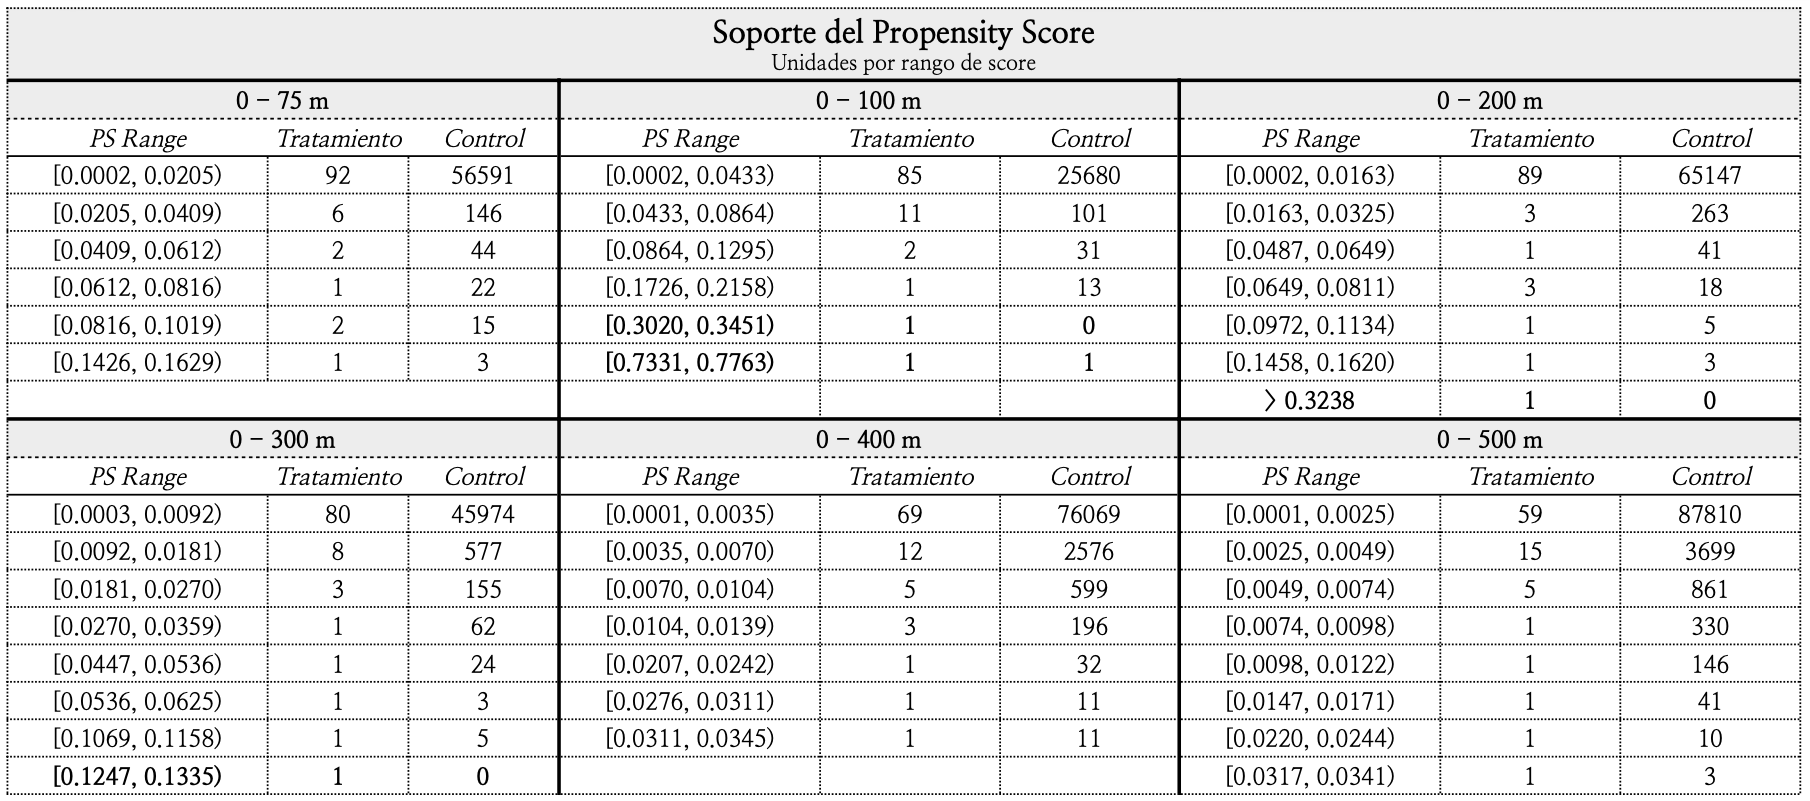
\includegraphics[width=\textwidth]{Imagenes/soporte-propensity-score.png}
\end{figure}

Con el objetivo de robustecer el emparejamiento, se evaluó la densidad de controles disponibles para cada rango del propensity score. \footnote{Para el cálculo de los rangos evaluados se consideró el rango de valores de los propensity scores de las unidades de control, partiendo dicho rango en 20 bins del mismo tamaño, y contando cuántas unidades tenían un propensity score en dicho rango} Se estableció un umbral mínimo de tres unidades de control por cada unidad tratada dentro de un mismo rango para poder proceder con el emparejamiento; en caso contrario, la unidad tratada se excluye del análisis. Tras aplicar este procedimiento de \textit{trimming}, se identificaron cuatro casos específicos donde fue necesario restringir la muestra: 
 
\begin{itemize}
    \item \textbf{Distancia de 50 metros}: Se excluyeron las unidades tratadas con un \textit{propensity score} mayor o igual a \textbf{0.3020}
    \item \textbf{Distancia de 200 metros}: Se excluyeron las unidades tratadas con un \textit{propensity score} mayor o igual a \textbf{0.3238}
    \item \textbf{Distancia de 300 metros}: Se excluyeron las unidades tratadas con un \textit{propensity score} mayor o igual a \textbf{0.1247}
\end{itemize}

Para el resto de las distancias y rangos analizados, las distribuciones muestran un solapamiento adecuado, lo que permite construir un universo de controles representativo y similar a las unidades tratadas sin necesidad de exclusiones adicionales

\subsection{Evaluación del balance mediante SMD}

Una vez definida la muestra con soporte común, se procedió a verificar la calidad del balance entre las unidades tratadas y sus respectivos contrafactuales. Para este propósito, se utilizó la \textit{Diferencia de Medias Estandarizada} (\textit{Standardized Mean Difference}, SMD), un indicador robusto que permite cuantificar el desequilibrio de las covariables sin depender del tamaño de la muestra. De acuerdo con el consenso en la literatura de inferencia causal, se considera que un proceso de emparejamiento es exitoso cuando los valores absolutos de SMD se sitúan por debajo del umbral de $0.1$, lo que garantiza que las unidades son estadísticamente comparables y que el sesgo de selección ha sido mitigado.

La Figura~[3.2] resume este diagnóstico para los distintos radios analizados (desde $37.5$ hasta $250$ metros), comparando la SMD antes (\textit{unadjusted}) y después (\textit{matched}) del procedimiento de emparejamiento.

\begin{figure}[htbp]
    \centering
    \caption{Comparación de SMD para radios evaluados}
    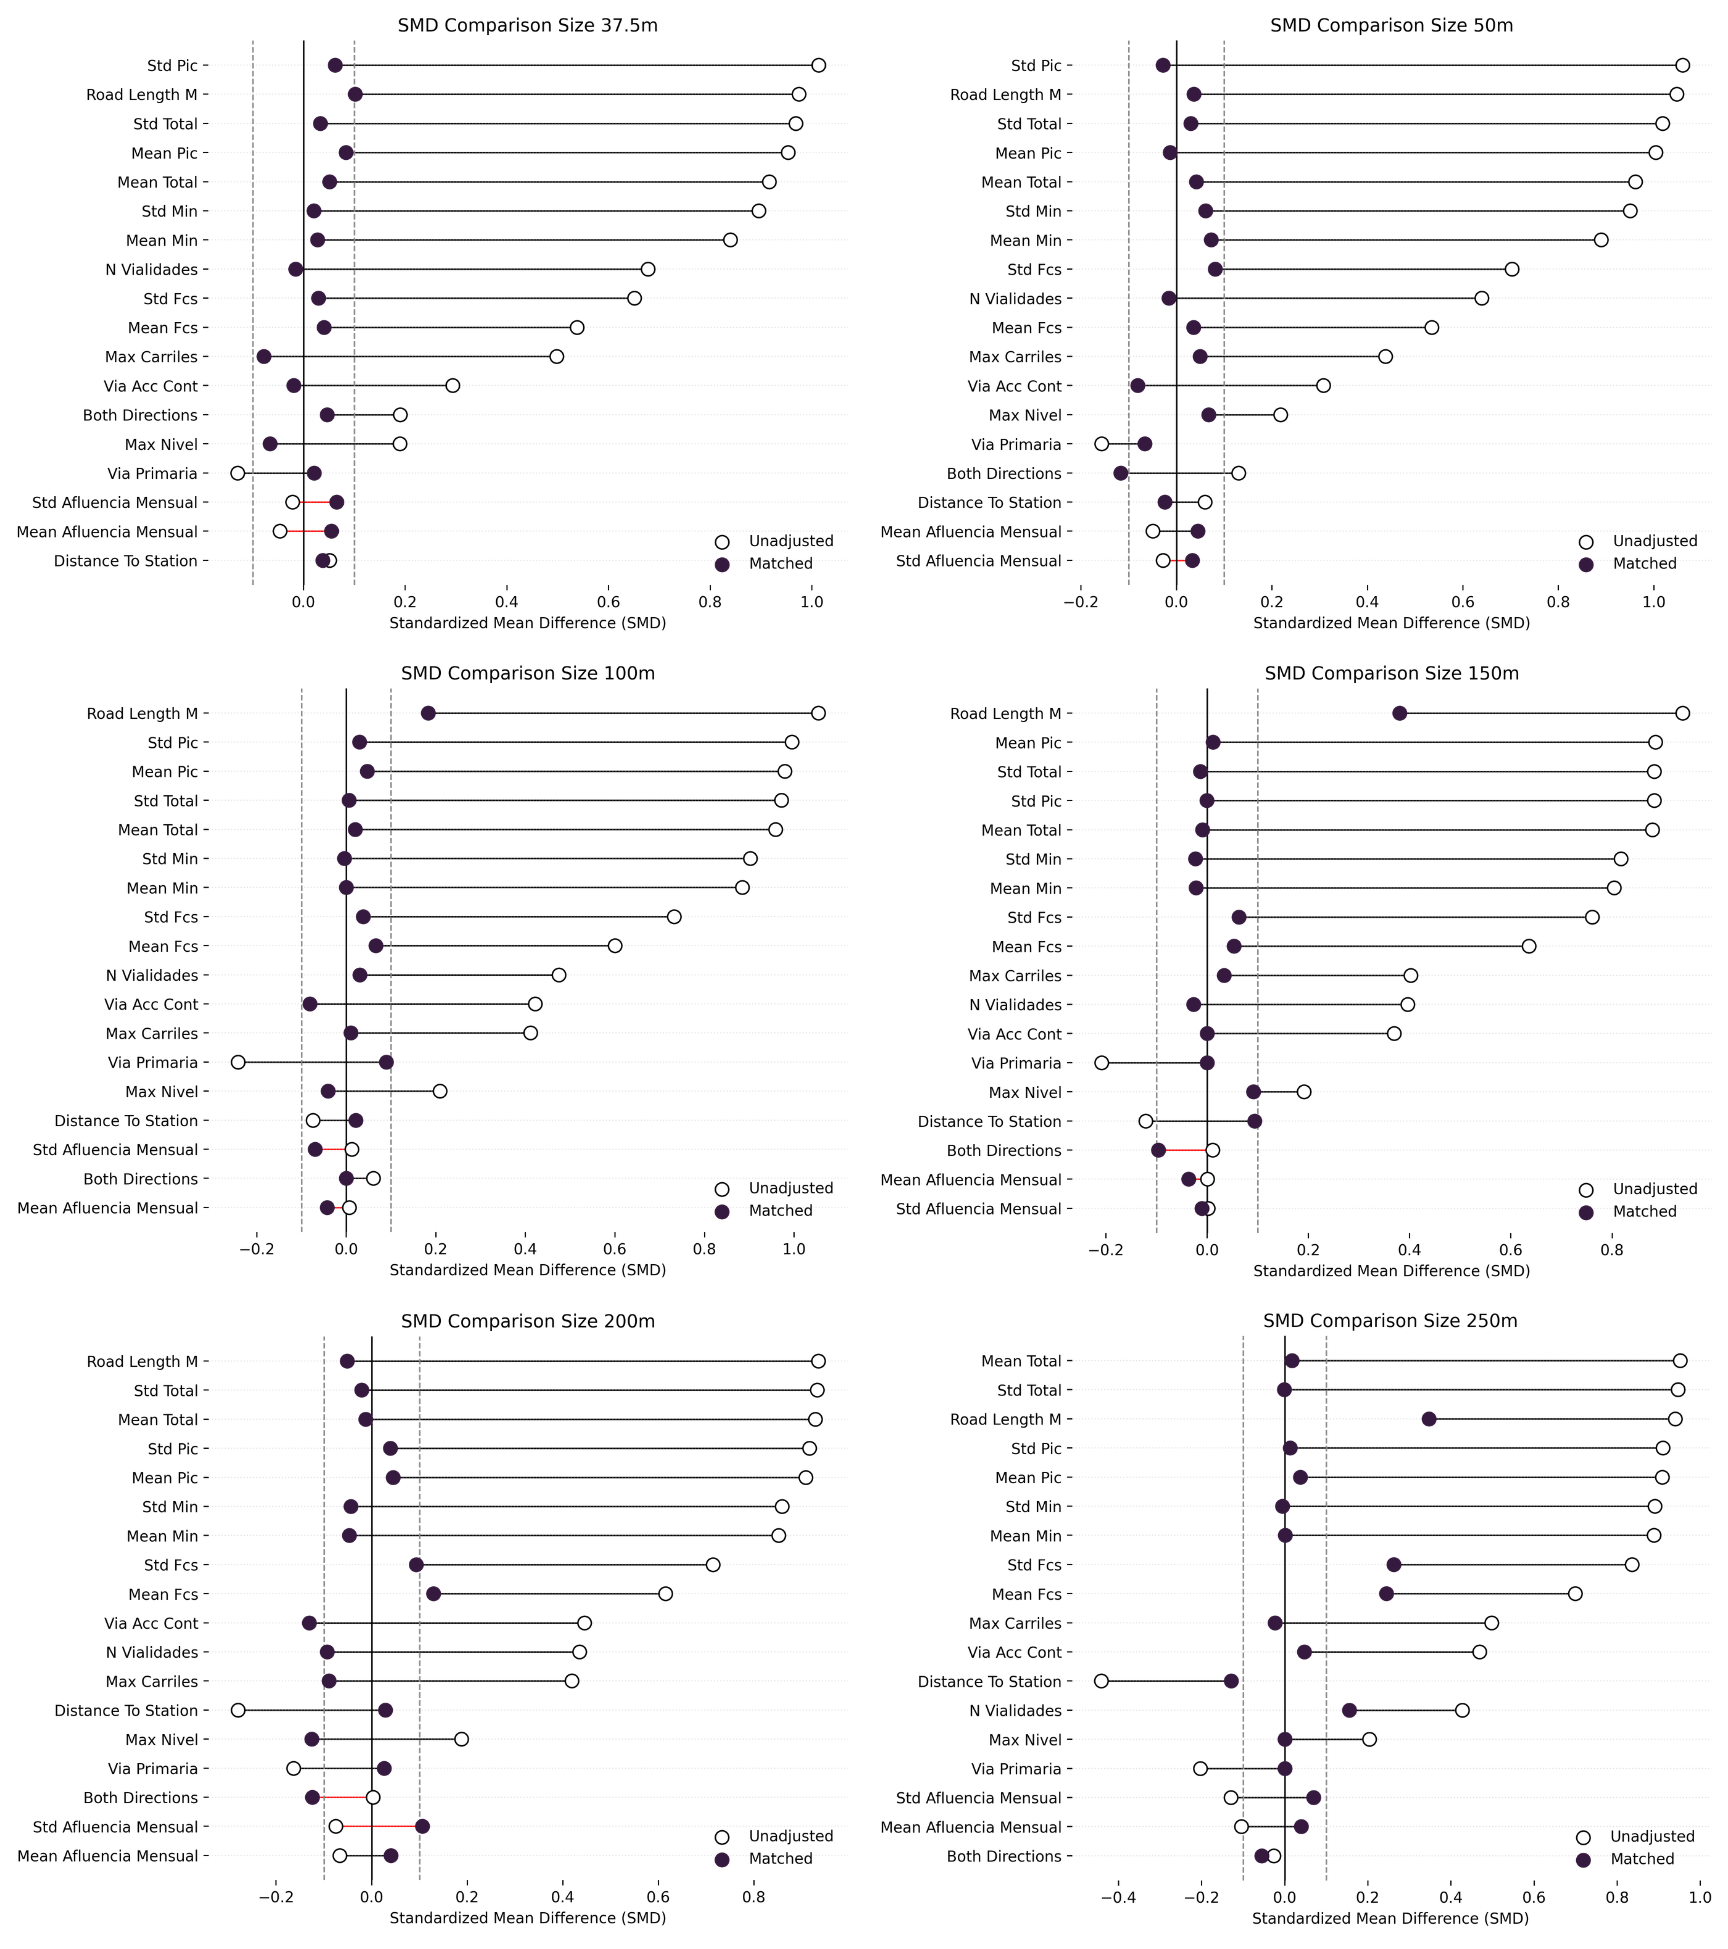
\includegraphics[width=\textwidth]{Imagenes/smd-comparisons.png}
\end{figure}

De manera consistente en todas las especificaciones, se observa una reducción sustancial en los valores de SMD para la mayoría de las covariables, lo que confirma que el algoritmo de \textit{nearest neighbor matching} logró construir grupos de control significativamente más similares a los tratados en comparación con la muestra original.

\begin{itemize}
    \item \textbf{Radios de alta precisión (37.5 m, 50 m y 100 m):} En estas escalas, el balance alcanzado es óptimo. En el radio de $50$ metros, prácticamente todas las variables —incluyendo el historial de siniestralidad pretratamiento y los \textit{proxies} de movilidad— se sitúan cerca del valor cero. Para las distancias de $37.5$ y $100$ metros, si bien variables como la distancia a estaciones de metro o la jerarquía vial presentan desbalances residuales mínimos, el SMD medio posterior al emparejamiento se mantiene por debajo del umbral crítico de $0.1$.
    \item \textbf{Radios intermedios (150 m y 200 m):}  A medida que el área de influencia se expande, la complejidad de las unidades espaciales aumenta. No obstante, el emparejamiento logra estabilizar la mayoría de las dimensiones críticas. En el radio de $200$ metros se observa una mayor dispersión en variables estructurales como el sentido de circulación (\textit{Both Directions}) y el nivel de la traza (\textit{Max Nivel}), aunque el balance global sigue permitiendo comparaciones válidas.
    \item \textbf{Radio de 250 m:}  En esta escala se registra la mayor variabilidad residual. Debido a la extensión del área, las unidades tratadas presentan configuraciones viales más heterogéneas, lo que dificulta encontrar controles perfectos en todas las dimensiones simultáneamente. Sin embargo, aun en este caso, el procedimiento de \textit{matching} reduce drásticamente el sesgo observado en la muestra original, mejorando la comparabilidad de las distribuciones respecto al escenario sin ajuste.
\end{itemize}

En conclusión, los diagnósticos de balance confirman que la estrategia de identificación es robusta. Aunque en los radios de mayor tamaño existen variables que superan levemente la cota de $0.1$, la mejora generalizada en la similitud de las covariables permite proceder con la estimación de los efectos mediante modelos de \textit{diferencia en diferencias}, bajo el supuesto de que las diferencias observadas en la siniestralidad no son producto de disparidades estructurales preexistentes entre los grupos, sino del efecto causal de los radares de velocidad.

\chapter{Estimación y Resultados}

\noindent Una vez consolidada la muestra emparejada mediante el \textit{propensity score matching}, se procede con la fase de estimación, para cuantificar el impacto que tuvieron los radares de velocidad. El objetivo último es identificar si la implementación del progarama de Fotoc\'ivicas generó un cambio significativo en la siniestralidad vial en las áreas tratadas.

\section{Definición de variables de resultados}
\noindent Para capturar el impacto real, el análisis se realiza sobre cuatro dimensiones de severidad, tratadas cada una como variables dependientes:

\begin{itemize}
    \item \textbf{Hechos de tránsito generales}: el agregado total de incidentes registrados
    \item \textbf{Incidentes menores (MIN)}: hechos de tránsito que no resultaron con personas lesionadas ni fallecimientos
    \item \textbf{Incidentes con lesionados (PIC)}: eventos que involucraron lesiones personales 
    \item \textbf{Incidentes fatales (FCS)}: hechos de tránsito donde se registró al menos una persona fallecida en el lugar
\end{itemize}

Adicionalmente, cada uno de estos incidentes se evalúa bajo dos métricas: en \textbf{nivles absolutos} (conteo mensual de incidentes por área), y en \textbf{tasas de siniestralidad}. Esta última métrica se construye normalizando el número de incidentes por cada $1,000$ vehículos que circularon en la ciudad durante el mes de de observación, utilizando los datos de los radares de conteo permanente para controlar por variaciones en la exposición vehicular. 

\section{Estimación}
\noindent Para poder estimar los efectos de las cámaras de velocidad sobre cada uno de los resultados definidos anteriormente, hago uso de dos modelos complementarios, uno que no incluye efectos fijos, y otro que sí lo hace. El primero está definido como sigue,

\[
    y_{it} = \alpha + \beta \cdot treat_i + \gamma \cdot post_t + \delta \cdot treat\_post_{it} + \epsilon_{it}
\]

Donde,
\begin{itemize}
    \item $y_{it}$ representa el outcome (total de accidentes o tasa) observado en la área $i$ durante el mes $t$
    \item $treat_i$ es una variable indicadora para las áreas que tienen un radar de velocidad. Es igual a $1$ si la área está tratada
    \item $post_t$ es una varialbe indicadora igual a $1$ para los meses posteriores al inicio del programa (abril de 2019)
    \item $treat\_post_{it}$ es el término de interacción que captura la exposición al tratamiento de las áreas. 
    \item $\beta$ es el parámetro de interés que estima el \textbf{efecto promedio del tratamiento sobre los tratados (ATT)}
\end{itemize}

\noindent Por otro lado, el modelo en el cual se incluyen efectos fijos queda definido de la siguiente forma,

\[
    y_{it} = \gamma_i + \lambda_t + \delta \cdot treat\_post_{it} + \epsilon_{it}
\]
En esta especificación, $\gamma_i$ corresponde a los efectos fijos por cada área, y captura todas las características invariantes en el tiempo, mientras que $\lambda_t$ son los efectos fijos por mes, y absorbe los cambios comunes en toda la ciudad en un mes determinado. El coeficiente $\delta$ es la estimación del impacto causal aislando todos los factores anteriores. 

La interpretación causal de esta estrategia descansa en tres elementos complementarios. Primero, que una vez condicionado el análisis a las unidades emparejadas por el \textit{propensity score} y a sus características geográficas, viales y de movilidad, la ubicación de los radares de velocidad pueda considerarse quasi aleatoria respecto a los resultados de siniestralidad. Segundo, que exista soporte común suficiente para construir contrafactuales razonables, condición que se satisface mediante el recorte de la muestra y las pruebas de balance presentadas anteriormente. Tercero, dado que el efecto se estima mediante diferencia en diferencias sobre la muestra emparejada, se requiere que en ausencia del programa las áreas tratadas y sus controles hubieran seguido trayectorias paralelas. Como se discute en el capítulo anterior, tanto la inspección visual de las series pretratamiento como las pruebas placebo resultan, en general, consistentes con este supuesto. 

\section{Resultados}
\noindent Tras la estimación de los modelos de diferencia en diferencias sobre la muestra emparejada, los resultados principales indican que \textbf{no existe evidencia estadística suficiente para afirmar que las cámaras de velocidad del programa de Fotoc\'ivicas generaron una reducción localizada de la siniestralidad} en su entorno inmediato.  

Como se observa en la tabla \ref{tab:results-main-general}, el coeficiente de interacción $treat\_post$ que captura el efecto promedio del tratamiento sobre los tratados (ATT), no alcanza niveles de significancia estadísticos ($p > 0.05$) en ninguna de las especificaciones analizadas. 

Las tablas \ref{tab:results-main-general}, \ref{tab:results-main-min}, \ref{tab:results-main-pic} y \ref{tab:results-main-fcs} permiten comparar simultáneamente los coeficientes estimados para cada radio en cada uno de los niveles de severidad de los incidentes, distinguiendo entre modelos sin efectos fijos y con efectos fijos, y entre resultados en niveles y en tasas.

\begin{table}[htbp]
    \centering
    \caption{Resultados sobre hechos de tránsito generales}
    \label{tab:results-main-general}
    \footnotesize
    \begin{adjustbox}{max width=\textwidth}
    \begin{tabular}{lcccccc}
        \toprule
        & 75 m & 100 m & 200 m & 300 m & 400 m & 500 m \\
        \midrule
        \multicolumn{7}{l}{\textit{Panel A. Total de accidentes, sin efectos fijos}} \\
        Intersección & $1.198^{***}$ & $1.444^{***}$ & $2.393^{***}$ & $3.177^{***}$ & $4.321^{***}$ & $5.578^{***}$ \\
         & $(0.030)$ & $(0.031)$ & $(0.045)$ & $(0.050)$ & $(0.062)$ & $(0.076)$ \\
        Tratamiento & $0.073^{*}$ & $0.074$ & $0.068$ & $-0.021$ & $-0.032$ & $0.066$ \\
         & $(0.043)$ & $(0.045)$ & $(0.064)$ & $(0.071)$ & $(0.087)$ & $(0.109)$ \\
        Tiempo & $-0.240^{***}$ & $-0.282^{***}$ & $-0.430^{***}$ & $-0.502^{***}$ & $-0.710^{***}$ & $-0.926^{***}$ \\
         & $(0.039)$ & $(0.041)$ & $(0.059)$ & $(0.066)$ & $(0.084)$ & $(0.100)$ \\
        Tratamiento x Tiempo & $0.012$ & $0.031$ & $0.040$ & $0.057$ & $0.097$ & $0.162$ \\
         & $(0.057)$ & $(0.061)$ & $(0.085)$ & $(0.096)$ & $(0.118)$ & $(0.144)$ \\
        \midrule
        \multicolumn{7}{l}{\textit{Panel B. Total de accidentes, con efectos fijos}} \\
        Tratamiento x Tiempo & $0.012$ & $0.031$ & $0.040$ & $0.057$ & $0.097$ & $0.162$ \\
         & $(0.057)$ & $(0.061)$ & $(0.085)$ & $(0.096)$ & $(0.118)$ & $(0.144)$ \\
        \midrule
        \multicolumn{7}{l}{\textit{Panel C. Tasa de accidentes, sin efectos fijos}} \\
        Intersección & $7.51 \times {10^{-5}}^{***}$ & $9.03 \times {10^{-5}}^{***}$ & $1.50 \times {10^{-4}}^{***}$ & $1.99 \times {10^{-4}}^{***}$ & $2.71 \times {10^{-4}}^{***}$ & $3.49 \times {10^{-4}}^{***}$ \\
         & $(1.85 \times 10^{-6})$ & $(1.91 \times 10^{-6})$ & $(2.81 \times 10^{-6})$ & $(3.14 \times 10^{-6})$ & $(3.90 \times 10^{-6})$ & $(4.74 \times 10^{-6})$ \\
        Tratamiento & $4.44 \times {10^{-6}}^{*}$ & $4.69 \times {10^{-6}}^{*}$ & $4.23 \times 10^{-6}$ & $-1.37 \times 10^{-6}$ & $-2.13 \times 10^{-6}$ & $4.12 \times 10^{-6}$ \\
         & $(2.67 \times 10^{-6})$ & $(2.83 \times 10^{-6})$ & $(4.00 \times 10^{-6})$ & $(4.46 \times 10^{-6})$ & $(5.46 \times 10^{-6})$ & $(6.78 \times 10^{-6})$ \\
        Tiempo & $-8.07 \times {10^{-6}}^{***}$ & $-8.95 \times {10^{-6}}^{***}$ & $-1.34 \times {10^{-5}}^{***}$ & $-1.29 \times {10^{-5}}^{***}$ & $-1.91 \times {10^{-5}}^{***}$ & $-2.48 \times {10^{-5}}^{***}$ \\
         & $(2.58 \times 10^{-6})$ & $(2.73 \times 10^{-6})$ & $(3.85 \times 10^{-6})$ & $(4.33 \times 10^{-6})$ & $(5.46 \times 10^{-6})$ & $(6.46 \times 10^{-6})$ \\
        Tratamiento x Tiempo & $1.33 \times 10^{-6}$ & $2.23 \times 10^{-6}$ & $3.35 \times 10^{-6}$ & $3.78 \times 10^{-6}$ & $6.44 \times 10^{-6}$ & $1.05 \times 10^{-5}$ \\
         & $(3.71 \times 10^{-6})$ & $(3.98 \times 10^{-6})$ & $(5.53 \times 10^{-6})$ & $(6.23 \times 10^{-6})$ & $(7.65 \times 10^{-6})$ & $(9.35 \times 10^{-6})$ \\
        \midrule
        \multicolumn{7}{l}{\textit{Panel D. Tasa de accidentes, con efectos fijos}} \\
        Tratamiento x Tiempo & $1.33 \times 10^{-6}$ & $2.23 \times 10^{-6}$ & $3.35 \times 10^{-6}$ & $3.78 \times 10^{-6}$ & $6.44 \times 10^{-6}$ & $1.05 \times 10^{-5}$ \\
         & $(3.71 \times 10^{-6})$ & $(3.98 \times 10^{-6})$ & $(5.53 \times 10^{-6})$ & $(6.23 \times 10^{-6})$ & $(7.65 \times 10^{-6})$ & $(9.35 \times 10^{-6})$ \\

        \bottomrule
    \end{tabular}
    \end{adjustbox}

    \vspace{0.4em}
    \begin{minipage}{0.93\textwidth}
        \tiny \textit{Nota:} Cada coeficiente aparece con su error estándar robusto entre paréntesis. ${}^{***} p<0.01$, ${}^{**} p<0.05$, ${}^{*} p<0.10$.
    \end{minipage}
\end{table}

\begin{table}[htbp]
    \centering
    \caption{Resultados sobre hechos de tránsito sin lesionados (MIN)}
    \label{tab:results-main-min}
    \footnotesize
    \begin{adjustbox}{max width=\textwidth}
    \begin{tabular}{lcccccc}
        \toprule
        & 75 m & 100 m & 200 m & 300 m & 400 m & 500 m \\
        \midrule
        \multicolumn{7}{l}{\textit{Panel A. Total de accidentes, sin efectos fijos}} \\
        Intersección & ${0.719}^{***}$ & ${0.823}^{***}$ & ${1.422}^{***}$ & ${1.894}^{***}$ & ${2.668}^{***}$ & ${3.428}^{***}$ \\
         & $(0.021)$ & $(0.021)$ & $(0.031)$ & $(0.035)$ & $(0.045)$ & $(0.055)$ \\
        Tratamiento & $0.025$ & ${0.076}^{**}$ & $0.015$ & $-0.030$ & $-0.086$ & $0.004$ \\
         & $(0.030)$ & $(0.032)$ & $(0.044)$ & $(0.051)$ & $(0.063)$ & $(0.078)$ \\
        Tiempo & ${-0.257}^{***}$ & ${-0.273}^{***}$ & ${-0.490}^{***}$ & ${-0.598}^{***}$ & ${-0.878}^{***}$ & ${-1.106}^{***}$ \\
         & $(0.026)$ & $(0.027)$ & $(0.039)$ & $(0.045)$ & $(0.056)$ & $(0.068)$ \\
        Tratamiento x Tiempo & $-0.004$ & $-0.031$ & $0.021$ & $0.022$ & $0.089$ & $0.081$ \\
         & $(0.038)$ & $(0.040)$ & $(0.055)$ & $(0.064)$ & $(0.079)$ & $(0.097)$ \\
        \midrule
        \multicolumn{7}{l}{\textit{Panel B. Total de accidentes, con efectos fijos}} \\
        Tratamiento x Tiempo & $-0.004$ & $-0.031$ & $0.021$ & $0.022$ & $0.089$ & $0.081$ \\
         & $(0.038)$ & $(0.040)$ & $(0.055)$ & $(0.064)$ & $(0.079)$ & $(0.097)$ \\
        \midrule
        \multicolumn{7}{l}{\textit{Panel C. Tasa de accidentes, sin efectos fijos}} \\
        Intersección & ${4.50 \times 10^{-5}}^{***}$ & ${5.15 \times 10^{-5}}^{***}$ & ${8.90 \times 10^{-5}}^{***}$ & ${1.19 \times 10^{-4}}^{***}$ & ${1.67 \times 10^{-4}}^{***}$ & ${2.15 \times 10^{-4}}^{***}$ \\
         & $(1.31 \times 10^{-6})$ & $(1.33 \times 10^{-6})$ & $(1.95 \times 10^{-6})$ & $(2.22 \times 10^{-6})$ & $(2.79 \times 10^{-6})$ & $(3.41 \times 10^{-6})$ \\
        Tratamiento & $1.47 \times 10^{-6}$ & ${4.70 \times 10^{-6}}^{**}$ & $9.86 \times 10^{-7}$ & $-1.88 \times 10^{-6}$ & $-5.48 \times 10^{-6}$ & $1.46 \times 10^{-7}$ \\
         & $(1.89 \times 10^{-6})$ & $(1.99 \times 10^{-6})$ & $(2.77 \times 10^{-6})$ & $(3.16 \times 10^{-6})$ & $(3.90 \times 10^{-6})$ & $(4.84 \times 10^{-6})$ \\
        Tiempo & ${-1.29 \times 10^{-5}}^{***}$ & ${-1.36 \times 10^{-5}}^{***}$ & ${-2.50 \times 10^{-5}}^{***}$ & ${-2.94 \times 10^{-5}}^{***}$ & ${-4.35 \times 10^{-5}}^{***}$ & ${-5.42 \times 10^{-5}}^{***}$ \\
         & $(1.71 \times 10^{-6})$ & $(1.76 \times 10^{-6})$ & $(2.48 \times 10^{-6})$ & $(2.88 \times 10^{-6})$ & $(3.63 \times 10^{-6})$ & $(4.39 \times 10^{-6})$ \\
        Tratamiento x Tiempo & $-2.02 \times 10^{-7}$ & $-1.60 \times 10^{-6}$ & $1.68 \times 10^{-6}$ & $1.40 \times 10^{-6}$ & $5.34 \times 10^{-6}$ & $5.26 \times 10^{-6}$ \\
         & $(2.45 \times 10^{-6})$ & $(2.60 \times 10^{-6})$ & $(3.55 \times 10^{-6})$ & $(4.12 \times 10^{-6})$ & $(5.09 \times 10^{-6})$ & $(6.25 \times 10^{-6})$ \\
        \midrule
        \multicolumn{7}{l}{\textit{Panel D. Tasa de accidentes, con efectos fijos}} \\
        Tratamiento x Tiempo & $-2.02 \times 10^{-7}$ & $-1.60 \times 10^{-6}$ & $1.68 \times 10^{-6}$ & $1.40 \times 10^{-6}$ & $5.34 \times 10^{-6}$ & $5.26 \times 10^{-6}$ \\
         & $(2.45 \times 10^{-6})$ & $(2.60 \times 10^{-6})$ & $(3.55 \times 10^{-6})$ & $(4.12 \times 10^{-6})$ & $(5.09 \times 10^{-6})$ & $(6.25 \times 10^{-6})$ \\
        \bottomrule
    \end{tabular}
    \end{adjustbox}

    \vspace{0.4em}
    \begin{minipage}{0.93\textwidth}
        \tiny \textit{Nota:} Cada coeficiente aparece con su error estándar robusto entre paréntesis. ${}^{***} p<0.01$, ${}^{**} p<0.05$, ${}^{*} p<0.10$.
    \end{minipage}
\end{table}

\begin{table}[htbp]
    \centering
    \caption{Resultados sobre hechos de tránsito con lesionados (PIC)}
    \label{tab:results-main-pic}
    \footnotesize
    \begin{adjustbox}{max width=\textwidth}
    \begin{tabular}{lcccccc}
        \toprule
        & 75 m & 100 m & 200 m & 300 m & 400 m & 500 m \\
        \midrule
        \multicolumn{7}{l}{\textit{Panel A. Total de accidentes, sin efectos fijos}} \\
        Intersección & ${0.470}^{***}$ & ${0.613}^{***}$ & ${0.956}^{***}$ & ${1.262}^{***}$ & ${1.631}^{***}$ & ${2.124}^{***}$ \\
         & $(0.015)$ & $(0.016)$ & $(0.022)$ & $(0.025)$ & $(0.030)$ & $(0.036)$ \\
        Tratamiento & ${0.047}^{**}$ & $-0.003$ & $0.050$ & $0.008$ & $0.049$ & $0.052$ \\
         & $(0.021)$ & $(0.023)$ & $(0.031)$ & $(0.035)$ & $(0.042)$ & $(0.051)$ \\
        Tiempo & $0.019$ & $-0.005$ & ${0.067}^{**}$ & ${0.103}^{***}$ & ${0.171}^{***}$ & ${0.183}^{***}$ \\
         & $(0.022)$ & $(0.024)$ & $(0.032)$ & $(0.036)$ & $(0.044)$ & $(0.051)$ \\
        Tratamiento x Tiempo & $0.018$ & ${0.059}^{*}$ & $0.017$ & $0.034$ & $0.015$ & $0.088$ \\
         & $(0.031)$ & $(0.034)$ & $(0.046)$ & $(0.052)$ & $(0.063)$ & $(0.076)$ \\
        \midrule
        \multicolumn{7}{l}{\textit{Panel B. Total de accidentes, con efectos fijos}} \\
        Tratamiento x Tiempo & $0.018$ & $0.059$ & $0.017$ & $0.034$ & $0.015$ & $0.088$ \\
         & $(0.031)$ & $(0.034)$ & $(0.046)$ & $(0.052)$ & $(0.063)$ & $(0.076)$ \\
        \midrule
        \multicolumn{7}{l}{\textit{Panel C. Tasa de accidentes, sin efectos fijos}} \\
        Intersección & ${2.95 \times 10^{-5}}^{***}$ & ${3.83 \times 10^{-5}}^{***}$ & ${5.99 \times 10^{-5}}^{***}$ & ${7.91 \times 10^{-5}}^{***}$ & ${1.02 \times 10^{-4}}^{***}$ & ${1.33 \times 10^{-4}}^{***}$ \\
         & $(9.35 \times 10^{-7})$ & $(1.02 \times 10^{-6})$ & $(1.38 \times 10^{-6})$ & $(1.55 \times 10^{-6})$ & $(1.86 \times 10^{-6})$ & $(2.22 \times 10^{-6})$ \\
        Tratamiento & ${2.93 \times 10^{-6}}^{**}$ & $-7.27 \times 10^{-8}$ & $3.09 \times 10^{-6}$ & $4.29 \times 10^{-7}$ & $3.06 \times 10^{-6}$ & $3.35 \times 10^{-6}$ \\
         & $(1.34 \times 10^{-6})$ & $(1.46 \times 10^{-6})$ & $(1.97 \times 10^{-6})$ & $(2.19 \times 10^{-6})$ & $(2.61 \times 10^{-6})$ & $(3.19 \times 10^{-6})$ \\
        Tiempo & ${4.99 \times 10^{-6}}^{***}$ & ${4.81 \times 10^{-6}}^{***}$ & ${1.20 \times 10^{-5}}^{***}$ & ${1.68 \times 10^{-5}}^{***}$ & ${2.43 \times 10^{-5}}^{***}$ & ${2.95 \times 10^{-5}}^{***}$ \\
         & $(1.46 \times 10^{-6})$ & $(1.61 \times 10^{-6})$ & $(2.17 \times 10^{-6})$ & $(2.41 \times 10^{-6})$ & $(2.95 \times 10^{-6})$ & $(3.41 \times 10^{-6})$ \\
        Tratamiento x Tiempo & $1.62 \times 10^{-6}$ & $3.66 \times 10^{-6}$ & $1.51 \times 10^{-6}$ & $2.36 \times 10^{-6}$ & $1.55 \times 10^{-6}$ & $5.68 \times 10^{-6}$ \\
         & $(2.10 \times 10^{-6})$ & $(2.31 \times 10^{-6})$ & $(3.11 \times 10^{-6})$ & $(3.48 \times 10^{-6})$ & $(4.19 \times 10^{-6})$ & $(5.06 \times 10^{-6})$ \\
        \midrule
        \multicolumn{7}{l}{\textit{Panel D. Tasa de accidentes, con efectos fijos}} \\
        Tratamiento x Tiempo & $1.62 \times 10^{-6}$ & $3.66 \times 10^{-6}$ & $1.51 \times 10^{-6}$ & $2.36 \times 10^{-6}$ & $1.55 \times 10^{-6}$ & $5.68 \times 10^{-6}$ \\
         & $(2.10 \times 10^{-6})$ & $(2.31 \times 10^{-6})$ & $(3.11 \times 10^{-6})$ & $(3.48 \times 10^{-6})$ & $(4.19 \times 10^{-6})$ & $(5.06 \times 10^{-6})$ \\
        \bottomrule
    \end{tabular}
    \end{adjustbox}

    \vspace{0.4em}
    \begin{minipage}{0.93\textwidth}
        \tiny \textit{Nota:} Cada coeficiente aparece con su error estándar robusto entre paréntesis. ${}^{***} p<0.01$, ${}^{**} p<0.05$, ${}^{*} p<0.10$.
    \end{minipage}
\end{table}

\begin{table}[htbp]
    \centering
    \caption{Resultados sobre hechos de tránsito con personas fallecidas (FCS)}
    \label{tab:results-main-fcs}
    \footnotesize
    \begin{adjustbox}{max width=\textwidth}
    \begin{tabular}{lcccccc}
        \toprule
        & 75 m & 100 m & 200 m & 300 m & 400 m & 500 m \\
        \midrule
        \multicolumn{7}{l}{\textit{Panel A. Total de accidentes, sin efectos fijos}} \\
        Intersección & ${0.009}^{***}$ & ${0.008}^{***}$ & ${0.015}^{***}$ & ${0.020}^{***}$ & ${0.022}^{***}$ & ${0.026}^{***}$ \\
         & $(0.002)$ & $(0.002)$ & $(0.002)$ & $(0.002)$ & $(0.003)$ & $(0.003)$ \\
        Tratamiento & $8.36 \times 10^{-4}$ & $9.42 \times 10^{-4}$ & $0.002$ & $0.001$ & $0.005$ & ${0.010}^{**}$ \\
         & $(0.002)$ & $(0.002)$ & $(0.003)$ & $(0.003)$ & $(0.004)$ & $(0.004)$ \\
        Tiempo & $-0.002$ & ${-0.004}^{*}$ & ${-0.007}^{***}$ & ${-0.006}^{**}$ & $-0.002$ & $-0.004$ \\
         & $(0.002)$ & $(0.002)$ & $(0.003)$ & $(0.003)$ & $(0.004)$ & $(0.004)$ \\
        Tratamiento x Tiempo & $-0.002$ & $0.002$ & $0.002$ & $3.95 \times 10^{-5}$ & $-0.007$ & $-0.007$ \\
         & $(0.003)$ & $(0.003)$ & $(0.004)$ & $(0.005)$ & $(0.005)$ & $(0.006)$ \\
        \midrule
        \multicolumn{7}{l}{\textit{Panel B. Total de accidentes, con efectos fijos}} \\
        Tratamiento x Tiempo & $-0.002$ & $0.002$ & $0.002$ & $3.95 \times 10^{-5}$ & $-0.007$ & $-0.007$ \\
         & $(0.003)$ & $(0.003)$ & $(0.004)$ & $(0.005)$ & $(0.005)$ & $(0.006)$ \\
        \midrule
        \multicolumn{7}{l}{\textit{Panel C. Tasa de accidentes, sin efectos fijos}} \\
        Intersección & ${5.62 \times 10^{-7}}^{***}$ & ${5.35 \times 10^{-7}}^{***}$ & ${9.54 \times 10^{-7}}^{***}$ & ${1.30 \times 10^{-6}}^{***}$ & ${1.40 \times 10^{-6}}^{***}$ & ${1.59 \times 10^{-6}}^{***}$ \\
         & $(9.90 \times 10^{-8})$ & $(9.75 \times 10^{-8})$ & $(1.28 \times 10^{-7})$ & $(1.51 \times 10^{-7})$ & $(1.62 \times 10^{-7})$ & $(1.78 \times 10^{-7})$ \\
        Tratamiento & $4.78 \times 10^{-8}$ & $5.54 \times 10^{-8}$ & $1.51 \times 10^{-7}$ & $7.85 \times 10^{-8}$ & $2.86 \times 10^{-7}$ & ${6.19 \times 10^{-7}}^{**}$ \\
         & $(1.43 \times 10^{-7})$ & $(1.41 \times 10^{-7})$ & $(1.88 \times 10^{-7})$ & $(2.17 \times 10^{-7})$ & $(2.39 \times 10^{-7})$ & $(2.74 \times 10^{-7})$ \\
        Tiempo & $-1.01 \times 10^{-7}$ & $-1.65 \times 10^{-7}$ & ${-3.72 \times 10^{-7}}^{**}$ & $-2.77 \times 10^{-7}$ & $9.20 \times 10^{-9}$ & $-6.96 \times 10^{-8}$ \\
         & $(1.39 \times 10^{-7})$ & $(1.34 \times 10^{-7})$ & $(1.67 \times 10^{-7})$ & $(2.11 \times 10^{-7})$ & $(2.43 \times 10^{-7})$ & $(2.62 \times 10^{-7})$ \\
        Tratamiento x Tiempo & $-8.88 \times 10^{-8}$ & $1.70 \times 10^{-7}$ & $1.71 \times 10^{-7}$ & $2.27 \times 10^{-8}$ & $-4.58 \times 10^{-7}$ & $-4.45 \times 10^{-7}$ \\
         & $(1.97 \times 10^{-7})$ & $(2.03 \times 10^{-7})$ & $(2.57 \times 10^{-7})$ & $(3.05 \times 10^{-7})$ & $(3.43 \times 10^{-7})$ & $(3.92 \times 10^{-7})$ \\
        \midrule
        \multicolumn{7}{l}{\textit{Panel D. Tasa de accidentes, con efectos fijos}} \\
        Tratamiento x Tiempo & $-8.88 \times 10^{-8}$ & $1.70 \times 10^{-7}$ & $1.71 \times 10^{-7}$ & $2.27 \times 10^{-8}$ & $-4.58 \times 10^{-7}$ & $-4.45 \times 10^{-7}$ \\
         & $(1.97 \times 10^{-7})$ & $(2.03 \times 10^{-7})$ & $(2.57 \times 10^{-7})$ & $(3.05 \times 10^{-7})$ & $(3.43 \times 10^{-7})$ & $(3.92 \times 10^{-7})$ \\
        \bottomrule
    \end{tabular}
    \end{adjustbox}

    \vspace{0.4em}
    \begin{minipage}{0.93\textwidth}
        \tiny \textit{Nota:} Cada coeficiente aparece con su error estándar robusto entre paréntesis. ${}^{***} p<0.01$, ${}^{**} p<0.05$, ${}^{*} p<0.10$.
    \end{minipage}
\end{table}


En el caso de los \textbf{hechos de tránsito generales}, los coeficientes estimados son consistentemente positivos -- lo que podría sugerir un ligero incremento relativo de incidentes en zonas tratadas --, sin embargo, carecen siempre de robustez estadística. 

Respecto a los incidentes fatales (FCS), la literatura sugiere que este es el rubro donde los radares suelen ser más efectivos. No obstante, en este análisis no se ha identificado dicho efecto, pues de nuevo, no se encuentra significancia en los resultados que puedan respaldarlo, incluso existe inconsistencia en los signos de los coeficientes, pues varían entre positivo y negativo, sin seguir alguna tendencia clara persistente con el aumento del radio de las áreas. 

Un resultado que vale la pena destacar es que en todas las regresiones realizadas la variable del \textbf{tiempo} ($post_t$) \textbf{es siempre negativa y estadísticamente significativa.} Este hallazgo indica que, tras la implementación de las Fotoc\'ivicas en abril de 2019, hubo una \textbf{reducción generalizada de la siniestralidad} en todas las áreas analizadas (tanto tratadas como de control). Dado que el grupo de control fue construido mediante \textit{propensity score matching}, este descenso sugiere dos hipótesis fundamentales:

\begin{enumerate}
    \item \textbf{Efecto generalizado}: dada la naturaleza pública de la ubicación de los radares y la transición hacia un modelo cívico-educativo, podría haber generado un cambio de comportamiento que va más allá de la ubicación puntual de los radares. Si los conductores estaban conscientes de que la ciudad cuenta con dichos sistemas, pueden haber cambiado su conducta no solo en las zonas con radares, sino también en zonas similares. 
    \item \textbf{Migración de incidentes}: la ausencia de un efecto localizado, sumado a la caída general en celdas comparables, puede sugerir que los incidentes migraron a otro tipo de zonas que son estructuralmente distintas a aquellas propensas a tener un radar de velocidad.
\end{enumerate}

Recordemos que el Gobierno de la Ciudad de México buscaba que las Fotoc\'ivicas generaran un cambio de conducta y no fueran un programa recaudatorio, razón por la cual hicieron pública la ubicación de todos los radares. Sin embargo, esta apertura es precisamente lo que puede haber diluido el efecto localizado: al saber dónde están las cámaras, es más fácil para los conductores evadir esas zonas o ajustar su velocidad solo en ese punto. Esta transparencia, sumada a que muchas sanciones todavía son económicas y no cívicas, podría estar fomentando una evasión sistemática que impide detectar un impacto puntual y directo en las celdas donde están los radares.

Los hallazgos de esta investigación presentan contrastes significativos con las evaluaciones oficiales y la literatura previa sobre el programa de Fotoc\'ivicas (SEMOVI, 2020; Madrigal y Rodríguez, 2021; Quintero et al., 2023). Mientras que la SEMOVI y Quintero et al. reportan reducciones porcentuales de hasta dos dígitos en la siniestralidad, los coeficientes de la variable de tiempo en este estudio sugieren que dicho descenso (situado entre el 15\% y 20\%) es de naturaleza sistémica y no localizada. Dado que Quintero et al. emplean una unidad de análisis a nivel municipal, es altamente probable que sus resultados capturen el efecto generalizado observado en toda la ciudad, independientemente de la presencia de radares en zonas específicas.

Por otro lado, a diferencia de Madrigal y Rodríguez (2021) --quien reconoce limitaciones en la construcción de su contrafactual--, esta tesis emplea el Propensity Score Matching (PSM) para garantizar que las unidades de control sean estadísticamente comparables, mitigando así el sesgo de selección, y derivado de ello, se observa que la significancia del impacto de los radares no existe. Si bien resulta complejo determinar si la reducción generalizada en los incidentes es atribuible exclusivamente al cambio de esquema sancionatorio o a factores exógenos no observados, la evidencia obtenida solo permite concluir que no existe un efecto causal localizado derivado de la ubicación física de las cámaras.

Leídos en conjunto, estos resultados permiten distinguir entre una caída agregada de la siniestralidad en la ciudad y un efecto causal atribuible a la presencia inmediata de una cámara. Esa distinción ayuda a entender parte de la evidencia previa para la CDMX: los estudios con unidades espaciales amplias pueden estar capturando cambios sistémicos del programa o del contexto urbano, mientras que una evaluación local con un contrafactual más estricto exige evidencia más puntual alrededor de los radares.


\chapter*{Conclusiones}
\addcontentsline{toc}{chapter}{Conclusiones}

% Las conclusiones tampoco cuentan como capítulo, ctm

\noindent En esta tesis, me propongo evaluar el impacto causal de las cámaras de velocidad en el número de incidentes viales en la Ciudad de México. Para lograr esto, evalúo el impacto de la transición del programa de \textit{Fotomultas} al sistema de \textit{Fotocívicas} en la Ciudad de México a partir de abril de 2019. El cambio no fue menor: implicó una redistribución de los radares de velocidad hacia zonas de alta siniestralidad y, sobre todo, una transformación en la lógica de sanción, priorizando el resarcimiento cívico y educativo sobre el fin meramente recaudatorio. Mi hipótesis inicial, como lo sugería la literatura, era que este despliegue generaría una reducción localizada de los incidentes viales, con especial énfasis en los eventos de mayor severidad a una distancia de 300 metros alrededor de los dispositivos. 

Para poder analizar el impacto, hago uso de dos estrategias complementarias: el \textit{Propensity Score Matching (PSM)}, para construir un grupo de control comparable, y los modelos de \textit{Diferencia en Diferencias}, para realizar la estimación de los efectos. Sin embargo, los resultados obtenidos tras este proceso contradicen la expectativa de un impacto puntual. Al comparar el grupo de control construido para ser estadísticamente similar --controlando por historial de accidentes, infraestructura vial y proxies de movilidad--, no se encontró evidencia estadística de que las cámaras generen una reducción localizada, ni en el número total de incidentes, ni en la tasa de incidentes en sus áreas de influencia. 

Más allá de estos hallazgos, la tesis deja cuatro aportes para la evaluación de políticas de control de velocidad en la Ciudad de México. El primero es una unidad espacial de análisis alineada con el carácter local del tratamiento, al estudiar radios centrados en cada cámara en lugar de áreas agregadas. El segundo es un contrafactual más creíble, construido mediante emparejamiento sobre siniestralidad previa, infraestructura vial y medidas de exposición. El tercero es una estrategia de medición que integra registros de la afluencia del Metro y estaciones permanentes de conteo de la SICT para incorporar cambios exógenos en movilidad durante la pandemia. El cuarto es interpretativo: distinguir entre efectos agregados del programa y efectos localizados de los radares permite visitar con mayor precisión la evidencia previa para la ciudad. 

Es importante destacar que esta ausencia de significancia en el efecto localizado no implica que la siniestralidad no haya disminuido. Por el contrario, algo que sí se pudo identificar fue que la variable que captura los cambios en el tiempo, mostró una reducción generalizada de la siniestralidad tanto en las áreas con una cámara de velocidad como en aquellas que no tienen una, siendo esta reducción de entre el 15\% y el 20\% tras la implementación del programa. Este dato, que coincide con las evaluaciones previas de la SEMOVI (2020), Quintero et. al (2022), sugiere que estos efectos no están necesariamente relacionados con la presencia física de un radar de velocidad, sino que más bien fueron reducciones generalizadas. 

Derivado de esto, surgen dos hipótesis principales que podrían explicar la coexistencia de una mejora sistémica frente a la ausencia de un efecto localizado. La primera reside en la posibilidad de que el programa de \textit{Fotocívicas} haya logrado efectivamente un cambio de comportamiento generalizado en la cultura vial de la Ciudad de México. Bajo esta lógica, la percepción de vigilancia y el carácter público de la ubicación de los radares habrían influido en la conducción de manera global, mitigando riesgos más allá de los puntos específicos de monitoreo. La segunda hipótesis sugiere un fenómeno de desplazamiento espacial: es posible que los conductores hayan modificado sus trayectorias habituales para evitar no solo las zonas con radares, sino también aquellas áreas con configuraciones viales similares donde se percibe una mayor probabilidad de sanción.

Lamentablemente, la falta de datos granulares sobre la afluencia vehicular a nivel de intersección impide validar de manera definitiva estas conjeturas. Sin una métrica precisa de flujo por tramo, no es posible distinguir si la reducción observada en los incidentes responde a una conducción más segura o simplemente a una redistribución del tráfico hacia vías no monitoreadas. Por lo tanto, con la evidencia disponible, mi análisis solo puede concluir que las cámaras de velocidad no presentan un efecto localizado estadísticamente significativo sobre el número de incidentes viales ni sobre su severidad en los radios estudiados.

A esta limitación se suma la complejidad de un esquema de sanciones que no es homogéneo. El hecho de que una proporción considerable de las infracciones siga teniendo un carácter económico --para vehículos con placas de otras entidades federativas-- introduce una variable de sesgo adicional. Esta dualidad en los incentivos podría estar diluyendo el impacto esperado de un sistema diseñado originalmente para el resarcimiento cívico, dificultando la identificación de si el resultado es atribuible a los radares o a la respuesta diferenciada de los usuarios ante el tipo de multa.

En última instancia, contar con datos que permitan medir con precisión el flujo vehicular en cada intersección será fundamental para futuras investigaciones. Esta información no solo permitiría robustecer la identificación del efecto causal, sino que también sentaría las bases para diseñar intervenciones más eficaces y propuestas de política pública que logren integrar de manera estratégica nuevos radares en el sistema de seguridad vial de la ciudad.


%----------------------------------------------------------------------------------------
%	APÉNDICES
%----------------------------------------------------------------------------------------

\begin{appendix}

% \include{Apendices/ApA}

\end{appendix}

%----------------------------------------------------------------------------------------
%	BIBLIOGRAFÍA
%----------------------------------------------------------------------------------------


\chapter*{Referencias}
\addcontentsline{toc}{chapter}{Referencias}

% Macro. Esto es muy importante, no lo borren

\makeatletter
\renewenvironment{thebibliography}[1]
     {\@mkboth{\MakeUppercase\refname}{\MakeUppercase\refname}%
      \list{}%
           {\setlength{\labelwidth}{0pt}%
            \setlength{\labelsep}{0pt}%
            \setlength{\leftmargin}{\parindent}%
            \setlength{\itemindent}{-\parindent}%
            \@openbib@code
            \usecounter{enumiv}}%
      \sloppy
      \clubpenalty4000
      \@clubpenalty \clubpenalty
      \widowpenalty4000%
      \sfcode`\.\@m}
     {\def\@noitemerr
       {\@latex@warning{Empty `thebibliography' environment}}%
      \endlist}
\makeatother


% Lista

% La manera recomendada para citar papers o libros en el formato de Chicago esta en el siguiente vínculo: https://www.chicagomanualofstyle.org/tools_citationguide/citation-guide-2.html

% Es importante poner el apellido del autor seguido del año de publicación, una coma y las páginas consultadas en el texto antes de puntuar y entre paréntesis para las citas en el cuerpo de la tesis

% Ejemplo:

% Las \textit{causas próximas} del crecimiento son conocidas: tecnología, capital humano y físico. La pregunta es ¿por qué unos países sí tienen estas causas próximas y otros no? La respuesta son las \textit{causas fundamentales:} suerte, geografía, cultura e instituciones (Acemoglu 2009, 110).

\begin{thebibliography}{}

\bibitem{}
Al-Masaeid, H. R., Mujalli, R. O., \& Al-Haj, E. H. (2020). Impact of fixed cameras on traffic crashes. \textit{Saudi Journal of Civil Engineering, 4}(10), 192–198. \url{https://doi.org/10.36348/sjce.2020.v04i10.001}

\bibitem{}
Arganis, J. (2022). \textit{Datos viales 2022}. Secretaría de Infraestructura, Comunicaciones y Transportes. \url{https://micrs.sct.gob.mx/images/DireccionesGrales/DGST/Datos_Viales_2022/00_Introducci%C3%B3n_DV2022.pdf}

\bibitem{}
Centro de Comando, Control, Cómputo, Comunicaciones y Contacto Ciudadano de la CDMX. (2024). \textit{Incidentes viales reportados por C5} [Dataset]. Consultado noviembre de 2025 en \url{https://datos.cdmx.gob.mx/dataset/incidentes-viales-c5}

\bibitem{}
Christie, S. M., Lyons, R. A., Dunstan, F. D., \& Jones, S. J. (2003). Are mobile speed cameras effective? A controlled before and after study. \textit{Injury Prevention, 9}(4), 302–306. \url{https://doi.org/10.1136/ip.9.4.302}

\bibitem{}
De Ceunynck, T. (2017). Installation of section control \& speed cameras. \textit{European Road Safety Decision Support System}, developed by the H2020 project SafetyCube. Recuperado el 26 de noviembre de 2025 de \url{http://www.roadsafety-dss.eu}

\bibitem{}
Dirección General de Servicios Técnicos. (2025). \textit{Datos viales}. Secretaría de Infraestructura, Comunicaciones y Transportes. \url{https://micrs.sct.gob.mx/index.php/infraestructura/direccion-general-de-servicios-tecnicos/datos-viales}

\bibitem{}
Esteva, J. (2025). \textit{Datos viales 2025}. Secretaría de Infraestructura, Comunicaciones y Transportes. \url{https://micrs.sct.gob.mx/images/DireccionesGrales/DGST/Datos_Viales_2025/00_DV2025_Introduccion.pdf}

\bibitem{}
Forjuoh, S. N. (2003). Traffic-related injury prevention interventions for low-income countries. \textit{Injury Control and Safety Promotion, 10}(1–2), 109–118. \url{https://doi.org/10.1076/icsp.10.1.109.14115}

\bibitem{}
García C, A. (2018). \textit{Guía para el control de la velocidad}. Secretaría de Salud / Secretariado Técnico del Consejo Nacional para la Prevención de Accidentes.

\bibitem{}
Graham, D. J., Naik, C., McCoy, E. J., \& Li, H. (2019). Do speed cameras reduce road traffic collisions? \textit{PLoS ONE, 14}(9), e0221267. \url{https://doi.org/10.1371/journal.pone.0221267}

\bibitem{}
Jiménez, J. (2020). \textit{Datos viales 2020}. Secretaría de Comunicaciones y Transportes. \url{https://micrs.sct.gob.mx/images/DireccionesGrales/DGST/Datos-Viales-2020/00_Introducci%C3%B3n_DV2020.pdf}

\bibitem{}
Jiménez, J. (2021). \textit{Datos viales 2021}. Secretaría de Comunicaciones y Transportes. \url{https://micrs.sct.gob.mx/images/DireccionesGrales/DGST/Datos_Viales_2021/00_Introducci%C3%B3n_DV2021.pdf}

\bibitem{}
Job, S., Cliff, D., Fleiter, J. J., Flieger, M., \& Harman, B. (2020). \textit{Guide for determining readiness for speed cameras and other automated enforcement}. Global Road Safety Facility and the Global Road Safety Partnership.

\bibitem{}
Li, H., Graham, D. J., \& Majumdar, A. (2013). The impacts of speed cameras on road accidents: An application of propensity score matching methods. \textit{Accident Analysis \& Prevention, 60}, 148–157. \url{https://doi.org/10.1016/j.aap.2013.08.003}

\bibitem{}
Li, H., Zhang, Y., \& Ren, G. (2020). A causal analysis of time-varying speed camera safety effects based on the propensity score method. \textit{Journal of Safety Research, 75}, 119–127. \url{https://doi.org/10.1016/j.jsr.2020.08.007}

\bibitem{}
Li, H., Zhu, M., Graham, D. J., \& Zhang, Y. (2020). Are multiple speed cameras more effective than a single one? Causal analysis of the safety impacts of multiple speed cameras. \textit{Accident Analysis \& Prevention, 139}, 105488. \url{https://doi.org/10.1016/j.aap.2020.105488}

\bibitem{}
Madrigal Montes de Oca, A., \& Rodríguez, A. (2021). El efecto de las fotoinfracciones en la Ciudad de México. \textit{Revista Espacialidades UAM, 11}(1), 83–97.

\bibitem{}
Mountain, L., Hirst, W., \& Maher, M. (2005). Are speed enforcement cameras more effective than other speed management measures? \textit{Accident Analysis \& Prevention, 37}(4), 742–754. \url{https://doi.org/10.1016/j.aap.2005.03.017}

\bibitem{}
Novoa, A. M., Pérez, K., Santamariña-Rubio, E., Marí-Dell’Olmo, M., Ferrando, J., Peiró, R., Tobías, A., Zori, P., \& Borrell, C. (2010). Impact of the penalty points system on road traffic injuries in Spain: A time–series study. \textit{American Journal of Public Health, 100}(11), 2220–2227. \url{https://doi.org/10.2105/ajph.2010.192104}

\bibitem{}
Nuño, J. (2023). \textit{Datos viales 2023}. Secretaría de Infraestructura, Comunicaciones y Transportes. \url{https://micrs.sct.gob.mx/images/DireccionesGrales/DGST/Datos_Viales_2023/00_Introducci%C3%B3n_DV2023.pdf}

\bibitem{}
Nuño, J. (2024). \textit{Datos viales 2024}. Secretaría de Infraestructura, Comunicaciones y Transportes. \url{https://micrs.sct.gob.mx/images/DireccionesGrales/DGST/Datos_Viales_2024/00_Int_DV2024.pdf}

\bibitem{}
Park, R. C., \& Hong, E. J. (2020). Urban traffic accident risk prediction for knowledge-based mobile multimedia service. \textit{Personal and Ubiquitous Computing, 26}(2), 417–427. \url{https://doi.org/10.1007/s00779-020-01442-y}

\bibitem{}
Rosenbaum, P. R., \& Rubin, D. B. (1983). The central role of the propensity score in observational studies for causal effects. \textit{Biometrika, 70}(1), 41–55. \url{https://doi.org/10.1093/biomet/70.1.41}

\bibitem{}
Rubin, D. (1972). Estimating causal effects of treatments in randomized and nonrandomized studies. \textit{ETS Research Bulletin Series, 1972}(2). \url{https://doi.org/10.1002/j.2333-8504.1972.tb00631.x}

\bibitem{}
Ruiz, G. (2015). \textit{Datos viales 2015}. Secretaría de Comunicaciones y Transportes. \url{https://micrs.sct.gob.mx/images/DireccionesGrales/DGST/Datos-Viales-2015/Introduccion_DV_2015.pdf}

\bibitem{}
Ruiz, G. (2016). \textit{Datos viales 2016}. Secretaría de Comunicaciones y Transportes. \url{https://micrs.sct.gob.mx/images/DireccionesGrales/DGST/Datos-Viales-2016/Introduccion_DV_2016.pdf}

\bibitem{}
Ruiz, G. (2017). \textit{Datos viales 2017}. Secretaría de Comunicaciones y Transportes. \url{https://micrs.sct.gob.mx/images/DireccionesGrales/DGST/Datos-Viales-2017/Introduccion_DV_2017.pdf}

\bibitem{}
Ruiz, G. (2018). \textit{Datos viales 2018}. Secretaría de Comunicaciones y Transportes. \url{https://micrs.sct.gob.mx/images/DireccionesGrales/DGST/Datos-Viales-2018/Introduccion_DV_2018.pdf}

\bibitem{}
Ruiz, G. (2019). \textit{Datos viales 2019}. Secretaría de Comunicaciones y Transportes. \url{https://micrs.sct.gob.mx/images/DireccionesGrales/DGST/Datos-Viales-2019/00_INTRODUCCI%C3%93N.pdf}

\bibitem{}
Secretaría de Movilidad. (2019). \textit{El sistema Fotocívicas entra en vigor este 22 de abril}. SEMOVI. Consultado el 26 de noviembre de 2025 en \url{https://www.semovi.cdmx.gob.mx/comunicacion/nota/el-sistema-fotocivicas-entra-en-vigor-este-22-de-abril}

\bibitem{}
Secretaría de Movilidad. (2023). \textit{Vialidades primarias de la Ciudad de México} [Dataset]. Consultado noviembre de 2025 en \url{https://datos.cdmx.gob.mx/dataset/vialidades-de-la-ciudad-de-mexico}

\bibitem{}
Secretaría de Movilidad. (2025). \textit{Afluencia diaria del metro CDMX} [Dataset]. Consultado noviembre de 2025 en \url{https://datos.cdmx.gob.mx/dataset/afluencia-diaria-del-metro-cdmx}

\bibitem{}
Secretaría de Seguridad Ciudadana. (2023). \textit{Fotocívicas (Ubicación)} [Dataset]. Consultado noviembre de 2025 en \url{https://datos.cdmx.gob.mx/dataset/fotocivicas}

\bibitem{}
Secretaría de Seguridad Ciudadana. (2025). \textit{Infracciones fotocívicas}. \url{https://www.ssc.cdmx.gob.mx/storage/app/media/Transito/Actualizaciones/infracciones-fotocivicas.pdf}

\bibitem{}
Treat, J. R. (1979). \textit{Tri-level study of the causes of traffic accidents: Final report}. Institute for Research in Public Safety, Indiana University.

\bibitem{}
Valverde, C. Q., Perez-Ferrer, C., Becerril, L. C., Santiago, A. M., Lopez, H. R., Galbarro, J. P., Quistberg, D. A., Roux, A. V. D., \& Barrientos-Gutierrez, T. (2022). Evaluation of road safety policies and their enforcement in Mexico City, 2015–2019: An interrupted time-series study. \textit{Injury Prevention, 29}(1), 35–41. \url{https://doi.org/10.1136/ip-2022-044590}

\bibitem{}
Van Der Sar, M., Mulder, I., \& Choenni, S. (2011). Camera use in the public domain: Towards a Big Sister approach. \textit{Workshop on Socio-Technical Aspects in Security and Trust (STAST)}, 30–36. \url{https://doi.org/10.1109/stast.2011.6059253}

\end{thebibliography}

\newpage
\thispagestyle{empty}
\begin{table}[p]
\centering
\small
\label{ed}
\begin{tabular}{c}
\textit{El efecto causal de las cámaras de velocidad}\\ \textit{en el número de incidentes viales}\\ \textit{en la Ciudad de México}\\ escrito por Mariano Alcaraz Aguilar,\\ se terminó de imprimir en (poner mes aquí) de 2026\\ en los talleres de (insertar aquí el nombre del taller).\\ (dirección del taller)\\ Ciudad de México.
\end{tabular}
\end{table}

% Si lo prefieren, avisen a su taller que esta página ya la incluyeron ustedes para que no les impriman las que ellos usan. Lo recomiendo ampliamente

%%%%%%%%%%%%%%%%%%%%%%%%%%%%%%%%%%%%%%%%%%%%%%%%%%%%%%%%%%%%%%%%%%%%%%%%%%%%%%%%%%%%%%%

\end{document}
